% Use the custom class defined in GDTReportClass.cls
\documentclass{GDTReportClass}

% Set document metadata using custom commands from the class file
\title{Module 1 -- Theory Notes}  % Titolo specifico del progetto
\subtitle{Mechanical and Acoustic Systems}
\info{Course held during A.A. 2025/2026 by prof. Fabio Antonacci}  % Sottotitolo coerente con la nomenclatura del corso
\course{Musical Acoustics}

\author{Giacomo De Toni}  % Authors
\PID{}
\SID{}  % Student ID numbers
\advisor{}  % Advisor's name

% Embed metadata for the PDF file
\begin{filecontents}{\jobname.xmpdata}
    \Title{Musical Acoustics 1}
    \Author{Giacomo De Toni}
    \Language{en-EN}
    \Keywords{Musical \sep Acoustics \sep Theory \sep PoliMI}
\end{filecontents}

\begin{document}

    % Generate the front matter (title page, abstract, table of contents, etc.)
    \input{01_FrontMatter/01_titlePage}     % Title page
    \settingfrontmatter  % Configure front matter settings
    \input{01_FrontMatter/03_summaries}     % Summaries

    % Configure main content settings (resets page numbering, chapter counters, etc.)
    \settingmaincontent  

    % Include the main chapters from separate files
    %! TEX rootmain.tex

\chapter{Discrete Systems}

Musical instruments can, at first glance, be described as assemblies of an exciter, a resonator and a sound emitter. In string instruments, for instance, the string is set into motion by plucking, striking or bowing; a bridge transmits energy to a resonant body and sound is radiated to the air. In wind instruments, airflow is perturbed (by a jet, reed or lip motion), shaped by the bore (the resonator) and emitted through the bell or tone holes. In all such examples, the organizing concept is oscillation, which is captured mathematically by harmonic motion.

\section{The Mass–Spring Model and the Harmonic Oscillator}

\begin{figure}[!htb]
    \centering
    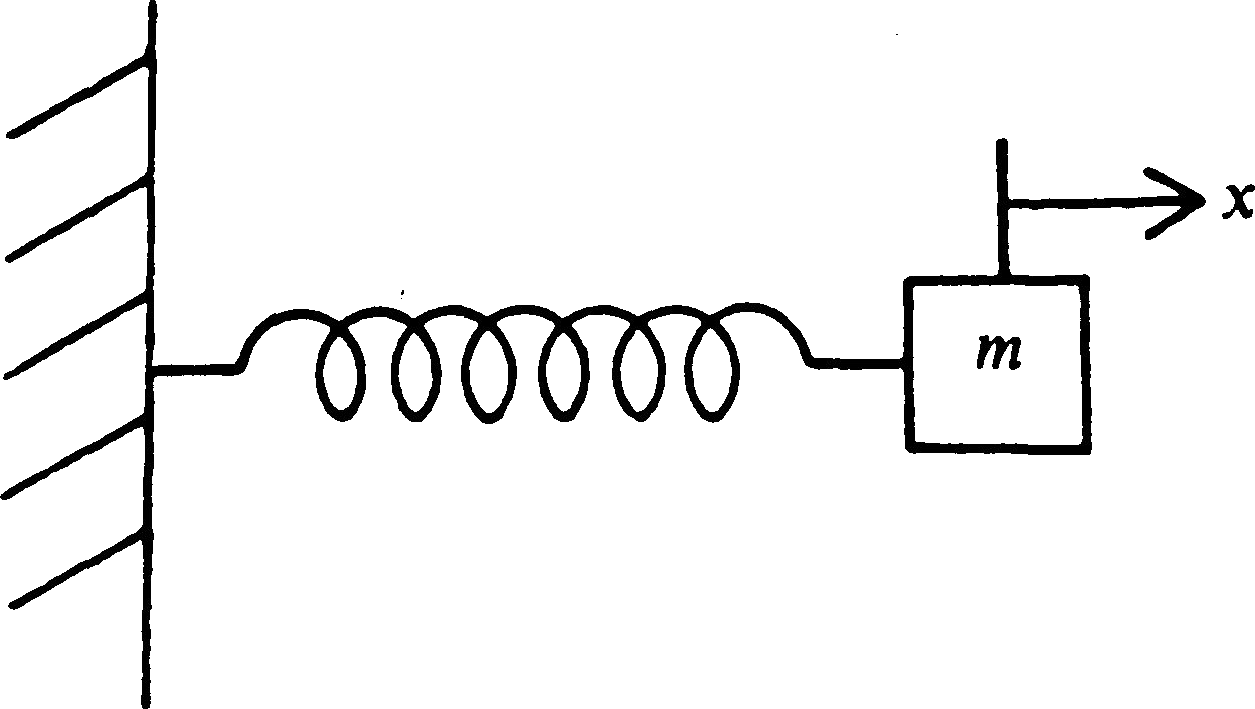
\includegraphics[width=0.5\linewidth]{00_Images/01_chapter/01.png}
    \caption{Simple mass-spring oscillator with mass \( m \), spring stiffness \( K \) and displacement \( x(t) \)}
    \label{fig:simpleosc}
\end{figure}

Consider the prototypical one-dimensional oscillator (as in figure \ref{fig:simpleosc}): a point mass \( m \) attached to a linear spring of stiffness \( K \). Neglecting dissipation, Newton’s second law combined with Hooke’s law yields
\[
m\ddot{x}(t) = - Kx(t)
\quad\Longleftrightarrow\quad
\ddot{x}(t) + \omega_0^2x(t) = 0,
\quad \text{with} \quad
\omega_0 = \sqrt{\frac{K}{m}}
\]
The quantity \( \omega_0 \) is the natural (or eigen) angular frequency of the system and \( f_0 = \omega_0/(2\pi) \) is the corresponding natural frequency. 

\subsection{General Solutions and Initial Conditions}

A complete solution of the homogeneous problem can be written in several equivalent forms, for example
\[
x(t) = A\cos(\omega_0 t + \phi)
\quad\text{or}\quad
x(t) = B\cos(\omega_0 t) + C\sin(\omega_0 t)
\]
where the two independent constants are fixed by the initial state \( (x_0, v_0) = \left(x(0), \dot{x}(0)\right) \). In the cosine-sine form one has \( x_0 = B \) and \( v_0 = \omega_0 C \); in amplitude--phase form,
\[
A = \sqrt{x_0^2 + \left(\frac{v_0}{\omega_0}\right)^2},
\qquad
\phi = \operatorname{atan2}\left( - \frac{v_0}{\omega_0},x_0\right)
\]
For completeness, the kinematic fields follow by differentiation:
\[
v(t) = \dot{x}(t) = - \omega_0 A \sin(\omega_0 t + \phi), 
\qquad
a(t) = \ddot{x}(t) = - \omega_0^2 A \cos(\omega_0 t + \phi) = -\omega_0^2 x(t)
\]
The velocity leads the displacement by \( \pi/2 \) and the acceleration is in antiphase with the displacement, as illustrated in figure \ref{fig:phasekin}. The motion is strictly periodic with period
\[
T = \frac{2\pi}{\omega_0}
\]
so that \( x(t + T) = x(t) \) for all \( t \).

\begin{figure}[!htb]
    \centering
    
\includegraphics[width=0.9\linewidth]{00_Images/01_chapter/02.png}
    \caption{Phase relations between \(x(t)\), \(v(t)\), and \(a(t)\) in harmonic motion}
    \label{fig:phasekin}
\end{figure}

\paragraph{Phase computation:} To determine the initial phase \( \phi \) from the initial state \( (x_0,v_0) \) of the harmonic oscillator \( x(t) = A\cos(\omega_0 t + \phi) \), one needs both \( \cos\phi = x_0/A \) and \( \sin\phi = - v_0/(A\omega_0) \). The ordinary inverse tangent \( \tan^{ - 1}(y/x) \) cannot resolve the correct quadrant of \( \phi \) and fails when \( x = 0 \). The two-argument function \( \operatorname{atan2}(y,x) \) returns the principal argument in \( ( - \pi,\pi] \) using the signs of \( x \) and \( y \), thus removing these ambiguities. Identifying the complex phasor \( \widetilde{A} = A e^{j\phi} = x_0 - j\frac{v_0}{\omega_0} \), one has \( \phi = \arg(\widetilde{A}) = \operatorname{atan2}\left( - \frac{v_0}{\omega_0},x_0\right) \). This is the computational counterpart of the complex-analytic principal argument and provides a numerically robust phase estimate consistent with the geometry of the initial data.

\section{Complex Exponential Representation}

It is often advantageous to represent sinusoidal motion using complex exponentials. Writing
\[
x(t) = A\cos(\omega_0 t + \phi) 
 = \Re\left[A e^{j\phi} e^{j\omega_0 t}\right] 
 = \Re\left[\widetilde{A} e^{j\omega_0 t}\right], 
\quad \text{with} \quad
\widetilde{A} = Ae^{j\phi}
\]
time differentiation becomes algebraic:
\[
v(t) = \left[j\omega_0 \widetilde{A}e^{j\omega_0 t}\right] = j\omega_0 x(t),
\qquad
a(t) = \left[(j\omega_0)^2 \widetilde{A}e^{j\omega_0 t}\right] = - \omega_0^2 x(t)
\]
In this form, differentiation corresponds to multiplication by \( j\omega_0 \), while integration corresponds to multiplication by \( 1/(j\omega_0) \).

\section{Linear Superposition of Harmonic Motions}

Many motions of practical interest are sums of a few simple harmonic oscillations. Because the governing dynamics are linear in the small–amplitude regime, displacements add algebraically and the resulting waveform can often be recast in a compact amplitude–phase form. Two representative cases are especially useful.

\subsection{Components at the Same Frequency}

Consider a family of cosines at the same angular frequency \( \omega_0 \),
\[
x(t) = \sum_{n = 1}^{N} A_n \cos\left(\omega_0 t + \phi_n\right)
\]
Introducing phasors \( \widetilde{A}_n = A_n e^{j\phi_n} \), the sum is a single cosine
\[
x(t) = A\cos\left(\omega_0 t + \phi\right)
\]
with resultant amplitude and phase
\[
A = \sqrt{\left(\sum_n A_n\cos\phi_n\right)^2 + \left(\sum_n A_n\sin\phi_n\right)^2},
\quad
\phi = \operatorname{atan2}\left(\sum_n A_n\sin\phi_n,\ \sum_n A_n\cos\phi_n\right)
\]
This recasting expresses vector addition in the complex plane.

\subsection{Two Components at Nearly Equal Frequencies (Beats)}

Let
\[
x(t) = A_1 \cos\left( \omega_1 t + \phi_1 \right) + A_2 \cos\left( (\omega_1 + \Delta \omega) t + \phi_2 \right),
\qquad 0 < \Delta\omega \ll \omega_1
\]
One may rewrite \( x(t) \) as a slowly modulated cosine at carrier \( \omega_1 \),
\[
x(t) = A(t)\cos\left(\omega_1 t + \phi(t)\right)
\]
where the slowly varying envelope \( A(t) \) and phase \( \phi(t) \) are
\[
A(t) = \sqrt{A_1^{2} + A_2^{2} + 2A_1A_2 \cos\left(\phi_1 - \phi_2 - \Delta \omega t\right)}
\]
\[
\phi(t) = \operatorname{atan2}\left( A_1 \sin \phi_1 + A_2 \sin \left( \phi_2 + \Delta \omega t \right), 
A_1 \cos \phi_1 + A_2 \cos \left( \phi_2 + \Delta \omega t \right) \right)
\]
The instantaneous amplitude varies between \( |A_1 - A_2| \) and \( A_1 + A_2 \) at the beat angular frequency \( \Delta\omega \) (beat frequency \( f_b = \Delta\omega/2\pi \)). In the symmetric special case \( A_1 = A_2 = A \) and \( \phi_1 = \phi_2 = 0 \),
\[
A(t) = A \sqrt{ 2 + 2 \cos( \Delta \omega t)} = 2 A \left| \cos \left( \frac{\Delta \omega}{2} t \right) \right|
\]
so that the envelope periodically collapses to zero and recovers to \( 2A \), producing the familiar beat pattern shown in figure \ref{fig:beats}.

\begin{figure}[!htb]
    \centering
    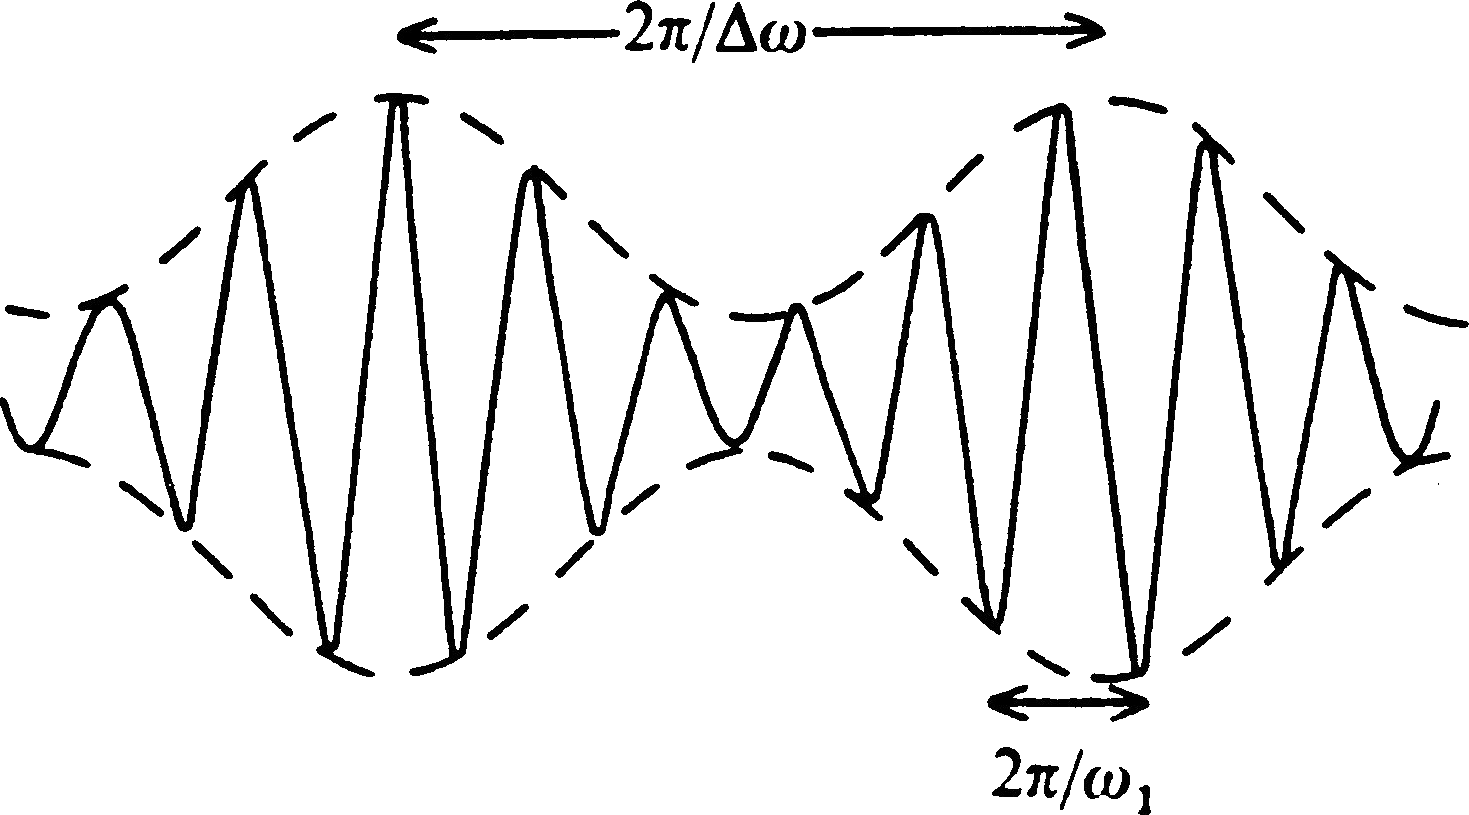
\includegraphics[width=0.5\linewidth]{00_Images/01_chapter/03.png}
    \caption{Beat waveform from the superposition of two nearly equal frequencies}
    \label{fig:beats}
\end{figure}

Importantly, this linear superposition contains only spectral lines at \( \omega_1 \) and \( \omega_1 + \Delta\omega \); it is not amplitude modulation in the nonlinear sense (which would also generate sidebands at \( \omega_1\pm \tfrac{\Delta\omega}{2} \)).

\section{Combinations of Springs and Masses}

When multiple springs act on the same degree of freedom, they may be reduced to an equivalent single spring. The most common layouts are summarized in figure \ref{fig:springcomb}. Two springs in parallel add their stiffnesses,
\[
K_P = K_1 + K_2
\]
whereas two in series combine as
\[
K_S = \frac{K_1K_2}{K_1 + K_2}
\]

\begin{figure}[!htb]
    \centering
    
\includegraphics[width=0.7\linewidth]{00_Images/01_chapter/04.png}
    \caption{Series and parallel combinations of springs and masses}
    \label{fig:springcomb}
\end{figure}

For equal springs \( K_1 = K_2 = K \) one finds \( K_{P} = 2K \) and \( K_{S} = K/2 \). These reductions allow many one-degree-of-freedom mass-spring layouts to be analyzed by substituting an effective stiffness \( K_{\text{eq}} \) and mass \( m_{\text{eq}} \) into
\[
\omega_0 = \sqrt{\frac{K_{\text{eq}}}{m_{\text{eq}}}},\qquad
f_0 = \frac{\omega_0}{2\pi}
\]

\section{Multidimensional Discrete Systems}

Real instruments and engineered structures seldom vibrate as a single lumped mass. A minimal example with more than one coordinate is the coupled two-mass system in figure \ref{fig:2dof}, which already exhibits multiple normal modes and distinct resonance features.

\begin{figure}[!htb]
    \centering
    
\includegraphics[width=0.5\linewidth]{00_Images/01_chapter/05.png}
    \caption{Two-degree-of-freedom mass-spring system}
    \label{fig:2dof}
\end{figure}

When multiple points can move, the dynamics are captured by the matrix form of Newton’s law for a linear, conservative, discrete system:
\[
\symbf{M} \vv{\ddot{\xi}}(t) + \symbf{K} \vv{\xi}(t) = \symbf{0}
\]
where \( \vv{\xi}(t) \in \mathbb{R}^{N} \) collects the generalized displacements of the \( N \) vibrating coordinates, \( \symbf{M}\in\mathbb{R}^{N\times N} \) is the symmetric mass matrix and \( \symbf{K} \in \mathbb{R}^{N\times N} \) is the symmetric stiffness matrix. Introducing the state vector \( \symbf{w} = [ \vv{\xi}^{T}  \vv{\dot{\xi}}^{T}]^{T} \) and the block matrix
\[
\symbf{\mathcal{M}_K} = 
\begin{bmatrix}
\symbf{0} & \symbf{I} \\
 - \symbf{M}^{ - 1}\symbf{K} & \symbf{0}
\end{bmatrix}
\]
the second-order system is embedded in first-order form \( \dot{\symbf{w}} = \symbf{\mathcal{M}_K} \symbf{w} \).

\subsection{Modal (Eigen) Analysis}

Normal modes arise from the eigenproblem of \( \symbf{\mathcal{M}_K} \). Seeking solutions \( \symbf{w}(t) = \vv{u}e^{\lambda t} \) with \( \symbf{\mathcal{M}_K} \vv{u} = \lambda \vv{u} \) and eliminating velocities yields the generalized eigenvalue problem in configuration space
\[
\symbf{K} \vv{\phi} = - \lambda^{2} \symbf{M} \vv{\phi}
\]
Writing \( \omega^{2} = - \lambda^{2} \ge 0 \), the natural (angular) frequencies \( \omega_n \) are the (real) roots of the characteristic equation
\[
\det \left( - \omega^{2}\symbf{M} + \symbf{K} \right) = 0
\]
with associated nontrivial eigenvectors (mode shapes) \( \vv{\phi}_n \) solving \( \left( - \omega_n^{2} \symbf{M} + \symbf{K} \right) \vv{\phi}_n = \vv{0} \). For conservative systems, the spectrum is finite (size \( N \)) and real. Mode shapes are defined up to a nonzero scalar factor.

\paragraph{Orthogonality and Consequences} Distinct modes \( m\neq n \) satisfy the orthogonality relations
\[
\vv{\phi}_n^{T} \symbf{M} \vv{\phi}_m = 0,
\qquad
\vv{\phi}_n^{T} \symbf{K} \vv{\phi}_m = 0
\]
which express that inertia and stiffness forces associated with one eigenmode do not do work in the motion of another-an energetic decoupling that underpins the mechanical independence of modes. Orthogonality and the resulting diagonalization in modal coordinates, strictly hold for undamped systems; with light proportional damping it remains approximately valid. Any motion can be expanded onto the modal basis, \( \vv{\xi}(t) = \sum_{n = 1}^{N} \vv{\phi}_nq_n(t) \), yielding \( N \) uncoupled scalar oscillators in the modal coordinates \( q_n(t) \).

\section{Damped Oscillations}

Real oscillators exhibit losses due to internal friction, radiation or other dissipation mechanisms. For a single degree of freedom with mass \( m \), viscous damping coefficient \( R \) and stiffness \( K \), the equation of motion reads
\[
m \ddot{x} + R \dot{x} + K x = 0
\quad \Longleftrightarrow \quad
\ddot{x} + 2 \alpha \dot{x} + \omega_0^{2} x = 0
\]
with \( \alpha = R/(2m) \) the (linear) damping rate and \( \omega_0 = \sqrt{K/m} \) the undamped natural angular frequency. Seeking exponential solutions \( x(t) = \widetilde{A} e^{\gamma t} \) gives the characteristic equation \( \gamma^{2} + 2 \alpha \gamma + \omega_0^{2} = 0 \), hence
\[
\gamma = - \alpha \pm j \omega_d,
\qquad
\omega_d = \sqrt{\omega_0^{2} - \alpha^{2}}
\]
For the underdamped case (\( 0 < \alpha < \omega_0 \)), the displacement is a decaying sinusoid,
\[
x(t) = e^{ - \alpha t} \left( A \cos \omega_d t + B \sin \omega_d t \right)
 = A_0 e^{ - \alpha t} \cos \left( \omega_d t + \phi \right)
\]
with constants fixed by the initial state \( (x_0,v_0) \). A convenient form is obtained by setting \( t = 0 \) in \( x \) and \( \dot{x} \):
\[
x(t) = e^{ - \alpha t} \left[ x_0 \cos(\omega_d t) + \frac{v_0 + \alpha x_0}{\omega_d} \sin(\omega_d t) \right]
\]
The motion is not strictly periodic, but the zero-crossing interval (and the interval between successive extrema) remains equal to the damped period \( T_d = 2\pi/\omega_d \). In many mechanical and acoustical systems of interest the damping is light, \( \alpha \ll \omega_0 \), so that \( \omega_d\simeq\omega_0 \). For \( \alpha = \omega_0 \) the system is critically damped and returns to equilibrium without oscillation; for \( \alpha > \omega_0 \) it is overdamped and exhibits a purely exponential relaxation governed by two real rates. The qualitative effect of increasing damping is summarized in figure \ref{fig:dampedcases}.

\begin{figure}[!htb]
    \centering
    
\includegraphics[width=0.9\linewidth]{00_Images/01_chapter/06.png}
    \caption{Free response for increasing damping: underdamped, critical, overdamped}
    \label{fig:dampedcases}
\end{figure}

\subsection{Decay Time and Quality Factor}

The amplitude envelope decays as \( e^{ - \alpha t} \). The decay time (or relaxation time) \( \tau \) is the time for the amplitude to drop by a factor \( e \), namely
\[
\tau = \frac{1}{\alpha} = \frac{2m}{R}
\]
An equivalent and widely used metric is the (dimensionless) quality factor \( Q \), which compares reactive to resistive effects and, for a lightly damped second-order resonator, is
\[
Q = \frac{\omega_0}{2\alpha} = \frac{K}{R\omega_0}
\]
Via \( \alpha = \omega_0/(2Q) \), the envelope over one (damped) period \( T_d \) decreases by the factor \( e^{ - \alpha T_d} \approx e^{ - \pi/Q} \) when \( \alpha \ll \omega_0 \). Typical values in musical acoustics span orders of magnitude: woodwind bores and wooden soundboards often exhibit \( Q \) between a few tens and a few hundreds, whereas plucked and struck strings can reach \( Q\sim10^{2} - 10^{4} \), depending on frequency range and construction. These figures reflect that each resonance behaves approximately as a single resonator with its own \( Q \).

\section{Air Resonators and Helmholtz Resonance}

Confined air can behave as an elastic element, storing and releasing potential energy through reversible compression. Simple archetypes, an air-filled cylinder closed by a moving piston and the Helmholtz resonator, admit compact lumped models that map pressure–volume dynamics onto the mass–spring oscillator. These models provide closed-form expressions for resonance frequencies in terms of geometry and thermophysical constants. Figure \ref{fig:helmholtzschemes} summarizes the key geometries and their mechanical analogies: a piston-cylinder resonator, the classical Helmholtz resonator with a neck, and a neckless cavity resonance.

\begin{figure}[!htb]
    \centering
    
\includegraphics[width=0.9\linewidth]{00_Images/01_chapter/07.png}
    \caption{Lumped-element analogies for air resonators: piston, Helmholtz, and neckless cavity}
    \label{fig:helmholtzschemes}
\end{figure}

\subsection{Piston in a Rigid Cylinder}

Consider a frictionless piston of mass \( m \) and area \( S \) sliding in a rigid, airtight cylinder of length \( L \). A small axial displacement changes the enclosed volume by \( \Delta V = Sx \) and produces a restoring pressure proportional to the fractional volume change. Under adiabatic conditions the effective (air) spring constant is
\[
K = \gamma p_a\frac{S}{L}
\]
where \( p_a \) is the ambient pressure and \( \gamma\simeq 1.4 \) is the ratio of specific heats for air. The piston–air system is thus a single-degree-of-freedom oscillator with natural frequency
\[
f_0 = \frac{1}{2\pi}\sqrt{\frac{K}{m}}
 = \frac{1}{2\pi}\sqrt{\frac{\gamma p_aS}{mL}}
\]
The dependence \( f_0\propto \sqrt{S/L} \) highlights that enlarging the cylinder (larger \( L \)) softens the effective spring, while increasing the piston area (larger \( S \)) stiffens it.

\subsection{Helmholtz Resonator with a Neck}

A Helmholtz resonator comprises a cavity of volume \( V \) vented by a short neck of length \( L \) and cross-section \( S \). The air slug in the neck behaves as the inertial mass
\[
m = \rho SL
\]
with \( \rho \) the air density, while the cavity acts as an acoustic spring with stiffness
\[
K = \rho\frac{S^{2}c^{2}}{V}
\]
where \( c \) is the speed of sound. The resonance frequency follows directly:
\[
f_0 = \frac{1}{2\pi}\sqrt{\frac{K}{m}}
 = \frac{c}{2\pi}\sqrt{\frac{S}{VL}}
\]
In this model, making the neck narrower (smaller \( S \)) lowers the resonance because the spring constant scales with \( S^2 \) while the inertial mass scales with \( S \), so the ratio \( K/m\propto S \) decreases.

\subsection{Neckless (Aperture) Resonator and End Correction}

When the cavity opens directly to the exterior without a physical neck, a virtual neck arises because a finite plug of exterior air moves in concert with the flow at the aperture. For a flanged circular opening of radius \( a \), the effective neck length is well approximated by twice the end correction \( \ell_e = \tfrac{8}{3\pi}a\approx 0.85a \), giving \( L_{\mathrm{eff}}\approx 2\ell_e\approx 1.7a \) for a large surrounding face. The corresponding neck mass and resonance frequency are then
\[
m = \rho SL_{\mathrm{eff}}
 = \rho(\pi a^{2})\left(\frac{16}{3\pi}a\right)
 = 5.33\rho a^{3},
\qquad
f_0 = \frac{c}{2\pi}\sqrt{\frac{1.85a}{V}}
\]
where the numerical factors reflect the end-correction geometry. If the baffle (face) around the hole is not large, the effective length is smaller and the actual frequency is slightly higher than this large-baffle estimate. 

\paragraph{Geometry note} The end correction depends on whether the opening is flanged or unflanged. Typical low-frequency values are \( \Delta L \approx 0.82a \) (flanged) and \( \Delta L \approx 0.61a \) (unflanged), so mixed conditions lead to intermediate \( L_{\mathrm{eff}} \).

\section{Forced Oscillations and Frequency Response Functions}

Free vibrations describe how a system evolves from an initial state. In musical acoustics, however, the most relevant situation is often the opposite: the resonator is driven by an external excitation (a bow force, an impact, an airflow perturbation) and we are interested in its steady-state response as a function of frequency. 

\subsection{Steady-State Harmonic Response}

\begin{figure}[!htb]
    \centering
    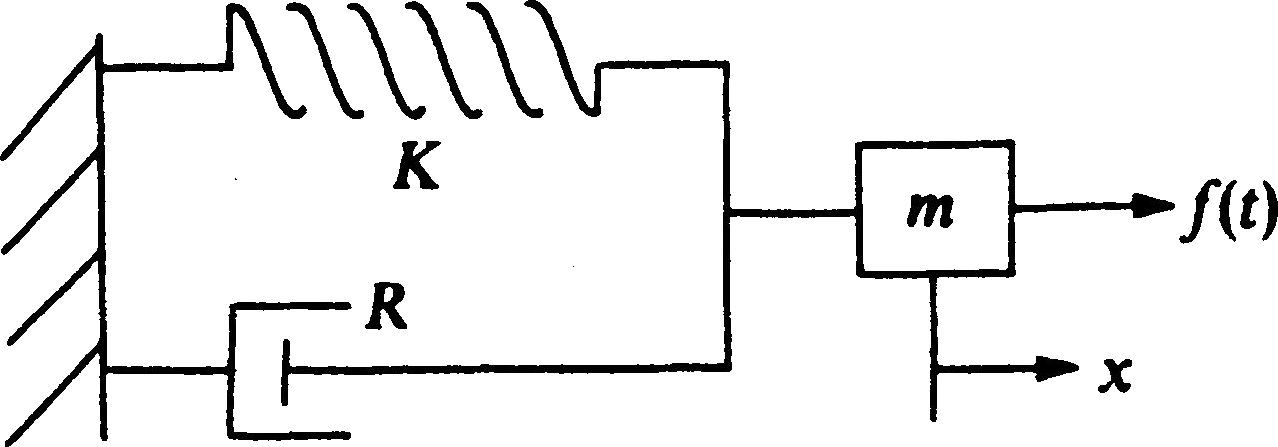
\includegraphics[width=0.5\linewidth]{00_Images/01_chapter/08.png}
    \caption{Damped oscillator driven by an external force \(F(t)\)}
    \label{fig:forcedosc}
\end{figure}

Let us consider the damped oscillator (figure \ref{fig:forcedosc}) driven by a sinusoidal force,
\[
m\ddot{x}(t) + R\dot{x}(t) + Kx(t) = F e^{j\omega t}
\]
Since the dynamics are linear, the steady-state response is harmonic at the same angular frequency \( \omega \). Introducing the complex ansatz
\[
x(t) = X(\omega)e^{j\omega t}
\]
substitution yields
\[
\left(K - \omega^{2}m + j\omega R\right)X(\omega) = F
\qquad\Rightarrow\qquad
X(\omega) = \frac{F}{K - \omega^{2}m + j\omega R}
\]
It is convenient to normalize by the mass and define
\[
\omega_0^2 = \frac{K}{m},\qquad \alpha = \frac{R}{2m}
\]
so that the displacement phasor becomes
\[
X(\omega) = \frac{F/m}{\omega_0^{2} - \omega^{2} + j2\alpha\omega}
\]
This is the frequency-domain description of the forced damped oscillator and it makes phase and amplitude immediately accessible.

\subsection{Mechanical Impedance and Mobility}

A particularly meaningful response quantity is the mechanical impedance, defined as the ratio between applied force and resulting velocity. Since
\[
V(\omega) = \dot{x}(t)e^{ - j\omega t} = j\omega \widetilde{X}(\omega)
\]
the impedance is
\[
Z(\omega) = \frac{F}{V(\omega)}
 = \frac{F}{j\omega X(\omega)}
 = R + j\left(\omega m - \frac{K}{\omega}\right)
 = R + jX(\omega)
\]
The real part \( R \) is the mechanical resistance, while the imaginary part is the mechanical reactance. The reactance crosses zero at resonance, since
\[
X(\omega_0) = \omega_0 m - \frac{K}{\omega_0} = 0
\]
and consequently, the impedance magnitude has a minimum around \( \omega = \omega_0 \). The inverse quantity
\[
Y(\omega) = \frac{1}{Z(\omega)} = \frac{V(\omega)}{F}
\]
is the mobility (or admittance). Writing \( Y = G + jB \), \( G \) is the conductance and \( B \) is the susceptance. Mobility is widely used in musical acoustics because radiated sound pressure is closely related to the vibrational velocity of the radiating surfaces. Typical trends of these quantities across resonance, together with the Nyquist representation, are illustrated in figure \ref{fig:impedance_mobility}.

\begin{figure}[!htb]
    \centering
    
\includegraphics[width=0.7\linewidth]{00_Images/01_chapter/09.png}
    \caption{Impedance and mobility of a damped oscillator in the frequency domain}
    \label{fig:impedance_mobility}
\end{figure}

\subsection{A Family of Vibrational FRFs}

Impedance and mobility are two members of a broader family of vibrational frequency response functions (FRFs), obtained by taking different output variables over the same input force:

\begin{align*}
&\Theta(\omega) = \frac{X(\omega)}{F(\omega)} \quad &\text{(receptance)}, 
\qquad
&\Sigma(\omega) = \frac{F(\omega)}{X(\omega)} \quad &\text{(dynamic stiffness)}
\\
&Y(\omega) = \frac{\dot{X}(\omega)}{F(\omega)} \quad &\text{(mobility)}, 
\qquad
&Z(\omega) = \frac{F(\omega)}{\dot{X}(\omega)} \quad &\text{(impedance)}
\\
&I(\omega) = \frac{\ddot{X}(\omega)}{F(\omega)} \quad &\text{(inertance)}, 
\qquad
&M(\omega) = \frac{F(\omega)}{\ddot{X}(\omega)} \quad &\text{(apparent mass)}
\end{align*}

In what follows, impedance and mobility will be emphasized, as they provide a direct link to velocity-driven sound radiation mechanisms. 

\subsection{Static Displacement, Resonance Gain and Asymptotic Behavior}

If the system is subject to a constant force \( F \), the static displacement is
\[
x_s = \frac{F}{K}
\]
At resonance (\( \omega = \omega_0 \)), it can be shown that the oscillation amplitude scales as
\[
|x(\omega_0)| = Qx_s
\]
so that the quality factor \( Q \) acts as an amplification factor of the static displacement. The reactance term in the impedance,
\[
X(\omega) = \omega m - \frac{K}{\omega}
\]
It also provides a useful physical interpretation. For \( \omega > \omega_0 \) the reactance is positive and dominated by \( \omega m \); hence, the system behaves mass-like. For \( \omega < \omega_0 \) the reactance is negative and dominated by \( - K/\omega \); hence, the system behaves spring-like. This is a general feature of second-order resonators: above resonance, they act as masses; below resonance, as springs.

\subsection{Receptance Bandwidth and the Q Factor}

The receptance of the damped oscillator has the characteristic form
\[
\Theta(\omega) = \frac{X(\omega)}{F(\omega)}
\propto
\frac{1}{\omega^{2} - 2j\alpha\omega - \omega_0^{2}}
\]
whose magnitude reaches a maximum near the damped resonance \( \omega = \omega_d \). Moreover, the magnitude drops by \SI{3}{\decibel} at
\[
\omega = \omega_d \pm \alpha
\]
so that the quantity \( 2 \alpha \) has the meaning of the (angular) bandwidth of the response:
\[
\Delta\omega \simeq 2\alpha
\]
Therefore, the quality factor
\[
Q = \frac{\omega_0}{2\alpha}
\]
can be interpreted as the ratio between the central frequency and the bandwidth (high \( Q \): sharp resonance; low \( Q \): broad resonance).

\subsection{Transient Response to a Suddenly Applied Harmonic Force}

The frequency response functions introduced above describe the steady-state motion under a harmonic excitation. In practice, however, the forcing is often applied at a finite time (e.g., an actuator is switched on at \( t = 0 \)), so the response generally contains a transient component in addition to the steady-state solution. Consider the damped oscillator driven by a sinusoidal force applied suddenly at rest,
\[
m\ddot{x}(t) + R\dot{x}(t) + Kx(t) = F\cos(\omega t) u(t)
\]
where \( u(t) \) is the Heaviside step. By linearity, the displacement can be written as the sum
\[
x(t) = x_{\mathrm{tr}}(t) + x_{\mathrm{ss}}(t)
\]
where \( x_{\mathrm{tr}} \) solves the homogeneous equation (free decay) and \( x_{\mathrm{ss}} \) is a particular (steady-state) solution at the driving frequency. For the underdamped case, the transient has the standard decaying oscillatory form
\[
x_{\mathrm{tr}}(t) = A e^{ - \alpha t} \cos\left(\omega_d t + \phi\right),
\qquad
\omega_d = \sqrt{\omega_0^2 - \alpha^2},
\qquad
\alpha = \frac{R}{2m}
\]
and, for light damping, \( \omega_d \simeq \omega_0 \). The steady-state motion is harmonic at the forcing frequency and may be written in amplitude-phase form as
\[
x_{\mathrm{ss}}(t) = X(\omega)\sin\left(\omega t + \varphi\right),
\qquad
X(\omega) = \frac{F}{\omega|Z(\omega)|}
\]
where \( Z(\omega) = R + j \left(\omega m - \frac{K}{\omega}\right) \) is the mechanical impedance. Therefore, the overall response can be expressed compactly as
\[
x(t) = A e^{ - \alpha t} \cos(\omega_d t + \phi) + \frac{F}{\omega|Z(\omega)|} \sin(\omega t + \varphi)
\]
Representative time histories for different values of \(\omega/\omega_0\) are shown in figure \ref{fig:sudden_sine}.

\begin{figure}[!htb]
    \centering
    
\includegraphics[width=0.7\linewidth]{00_Images/01_chapter/10.png}
    \caption{Response to a sinusoid applied suddenly at \( t = 0 \) for different \( \omega/\omega_0 \)}
    \label{fig:sudden_sine}
\end{figure}

\paragraph{Beatings and build-up} During the transient, the displacement exhibits components at the natural frequency (approximately \( f_0 \)) and at the driving frequency \( f = \omega/2\pi \). If \( f \) is close enough to \( f_0 \), the superposition of these two oscillatory components produces beatings in the observed waveform. As damping increases, the natural-frequency component decays faster and beatings disappear more quickly. In the special case \( \omega = \omega_0 \), the response builds up to the steady-state solution without beats: regardless of the initial transient details, the motion eventually settles into the forced oscillation at frequency \( \omega \).

\section{Forced Multidimensional Discrete Systems}

When a multidimensional discrete system is excited by a distribution of external forces, its motion is governed by the forced matrix equation
\[
\symbf{M}\vv{\ddot{\xi}}(t) + \symbf{K}\vv{\xi}(t) = \vv{f}(t)
\]
Spectral theory ensures that the eigenmodes of the associated conservative system form a complete basis for the space spanned by \( \vv{\xi} \). As a consequence, any response admits a unique expansion onto the modal basis,
\[
\vv{\xi}(t) = \sum_{n = 1}^{N}\vv{\phi}_n q_n(t)
\]
where \( q_n(t) \) are the generalized displacements, also referred to as modal participation factors. 

\subsection{Undamped Case: Modal Forces and Resonant FRFs}

Substituting the modal expansion into the forced equation of motion and taking the inner product with an eigenvector \( \vv{\phi}_m \) orthogonality eliminates cross-terms and yields one scalar oscillator per mode:
\[
\langle \vv{\phi}_n,\symbf{M}\vv{\phi}_n\rangle \ddot{q}_n(t)
 + \langle \vv{\phi}_n,\symbf{K}\vv{\phi}_n\rangle q_n(t)
 = \langle \vv{\phi}_n,\vv{f}(t)\rangle
\]
It is natural to introduce the modal quantities
\[
m_n = \langle \vv{\phi}_n,\symbf{M}\vv{\phi}_n\rangle,
\qquad
\kappa_n = \langle \vv{\phi}_n,\symbf{K}\vv{\phi}_n\rangle,
\qquad
f_n(t) = \langle \vv{\phi}_n,\vv{f}(t)\rangle
\]
so that, using \( \kappa_n = m_n\omega_n^2 \), each modal coordinate satisfies
\[
\ddot{q}_n(t) + \omega_n^2 q_n(t) = \frac{f_n(t)}{m_n}
\]
The scalar forcing term \( f_n \) is the projection of the force distribution onto mode \( n \): if \( f_n(t) = 0 \), then mode \( n \) cannot be excited by that forcing. Physically, this occurs, for instance, when a string drives a soundboard at a point coinciding with a nodal line of a given soundboard mode. In the frequency domain, for a harmonic forcing at angular frequency \( \omega \), the modal receptance reads
\[
Q_n(\omega) = \frac{f_n(\omega)}{m_n} \frac{1}{\omega_n^2 - \omega^2}
\]
and the configuration-space response becomes a sum of resonant terms,
\[
\vv{\Xi}(\omega) = \sum_{n = 1}^{N} \vv{\phi}_n\frac{f_n(\omega)}{m_n} \frac{1}{\omega_n^2 - \omega^2}
\]
Consequently, if the system is forced at a frequency \( \omega \) close to a given eigenfrequency \( \omega_n \), that modal contribution dominates and (in the ideal undamped limit) its amplitude tends to infinity.

\paragraph{Normalization invariance} Because each eigenvector is defined up to a multiplicative constant \( C \), one has \( m_n \propto C^2 \) while \( f_n \propto C \), hence \( q_n \propto C^{ - 1} \). The physical displacement \( \vv{\xi} = \sum_n \vv{\phi}_n q_n \) is therefore independent of the chosen normalization of the mode shapes. 

\subsection{Damped Case: Modal Coupling and Weak-Damping Correction}

In a linear system with a finite number of degrees of freedom, viscous dissipation can be modeled as a non-negative quadratic form of the velocity,
\[
\mathcal{D}(\vv{\dot{\xi}}) = \frac{1}{2}\vv{\dot{\xi}}^{T}\symbf{C}\vv{\dot{\xi}}
\]
where \( \symbf{C} \) is a symmetric damping matrix. The forced equations of motion then become
\[
\symbf{M}\vv{\ddot{\xi}}(t) + \symbf{C}\vv{\dot{\xi}}(t) + \symbf{K}\vv{\xi}(t) = \vv{F}(t)
\]
Expanding \( \vv{\xi}(t) = \sum_m \vv{\phi}_m q_m(t) \) onto the conservative eigenmodes and projecting onto \( \vv{\phi}_n \) yields
\[
\langle \vv{\phi}_n,\symbf{M}\vv{\phi}_n\rangle \ddot{q}_n
 + \sum_{m}\langle \vv{\phi}_n,\symbf{C}\vv{\phi}_m\rangle \dot{q}_m
 + \langle \vv{\phi}_n,\symbf{K}\vv{\phi}_n\rangle q_n
 = \langle \vv{\phi}_n,\vv{F}\rangle
\]
Defining the inter-modal damping coefficients through
\[
\langle \vv{\phi}_n,\symbf{C}\vv{\phi}_m\rangle = 2\zeta_{mn}m_n\omega_n
\]
one obtains the coupled system for the generalized coordinates.
\[
\ddot{q}_n + 2\omega_n\sum_{m}\zeta_{mn}\dot{q}_m + \omega_n^2 q_n
 = \frac{f_n}{m_n}
\]
In general, \( \symbf{C} \) cannot be diagonalized in the same basis as \( \symbf{M} \) and \( \symbf{K} \), so \( \zeta_{mn} \) with \( m \neq n \) are not zero and the modes are coupled through velocity terms. It is common to separate the diagonal (modal) damping coefficient \( \zeta_n \) from the off-diagonal coupling terms, rewriting
\[
\ddot{q}_n + 2\omega_n\zeta_n\dot{q}_n + \omega_n^2 q_n
 = \frac{f_n}{m_n} - 2\omega_n\sum_{m\neq n}\zeta_{mn}\dot{q}_m
\]
Under the assumption of weak damping, one may seek first-order corrections of the conservative eigenpairs,
\[
\omega_n' = \omega_n + \Delta\omega_n,
\qquad
\vv{\phi}_n' = \vv{\phi}_n + \Delta\vv{\phi}_n
\]
leading to the approximation
\[
\Delta\omega_n \simeq j\zeta_n\omega_n
\]
Hence, the correction to the eigenfrequency is purely imaginary: the corresponding eigensolution becomes a damped sinusoid, slowly decaying when damping is weak. Moreover, at first order, the inter-modal damping terms do not affect \( \Delta\omega_n \), which is equivalent to approximating \( \symbf{C} \) as diagonal in the modal basis. Finally, the weak-damping correction to the eigenshapes can be expressed as
\[
\vv{\phi}_n'
 = 
\vv{\phi}_n
 + 
2jm_n\omega_n^2
\sum_{m\neq n}
\vv{\phi}_m
\frac{\zeta_{mn}}{m_m(\omega_n^2 - \omega_m^2)}
\]
If neighboring eigenfrequencies are well separated, the correction remains small (of the order of \( \zeta_{mn} \)); conversely, for closely spaced modes, the denominator \( \omega_n^2 - \omega_m^2 \) can magnify the perturbation and significantly alter the shapes. Since the correction is purely imaginary, the damped mode shapes are no longer everywhere in phase (or in anti-phase) as in the conservative limit. 

\section{Forced Vibration of a Two-Mass System}

A simple yet widely applicable coupled resonator is the two-mass system in which a sinusoidal driving force acts on one mass only. This layout is a prototype for a bass-reflex loudspeaker, a guitar with fixed ribs and the dynamic absorber used to suppress machine vibrations. A particularly important case is the driven two-mass system in figure \ref{fig:twomass_forced}, together with its equivalent electrical circuit representation, which makes clear the close analogy between mechanical and electrical networks.

\begin{figure}[!htb]
    \centering
    
\includegraphics[width=0.7\linewidth]{00_Images/01_chapter/11.png}
    \caption{Driven two-mass system and its electrical analogue}
    \label{fig:twomass_forced}
\end{figure}

\subsection{Equations of Motion}

Let \( x_1(t) \) and \( x_2(t) \) denote the displacements of \( m_1 \) and \( m_2 \). With spring constants \( K_1 \) (to ground) and \( K_2 \) (coupling spring) and a harmonic force \( F_0\sin(\omega t) \) applied to \( m_1 \), the equations of motion are
\[
m_1\ddot{x}_1 + K_1 x_1 + K_2(x_1 - x_2) = F_0 \sin(\omega t),
\qquad
m_2\ddot{x}_2 + K_2(x_2 - x_1) = 0
\]
This is the minimal discrete model in which coupling generates two resonance frequencies, in contrast to the single peak of a one-degree-of-freedom oscillator.

\subsection{Harmonic Solution, Resonances and Antiresonance}

Seeking steady-state solutions at the driving frequency,
\[
x_1(t) = \Re\left\{X_1(\omega)e^{j\omega t}\right\},
\qquad
x_2(t) = \Re\left\{X_2(\omega)e^{j\omega t}\right\}
\]
one obtains the algebraic system
\[
\begin{bmatrix}
K_1 + K_2 - \omega^2 m_1 & - K_2\\
 - K_2 & K_2 - \omega^2 m_2
\end{bmatrix}
\begin{bmatrix}
X_1 \\ X_2
\end{bmatrix}
 = 
\begin{bmatrix}
F_0 \\ 0
\end{bmatrix}
\]
Solving by elimination yields the response amplitudes
\[
X_1(\omega) = 
\frac{(K_2 - \omega^2 m_2)F_0}
{(K_1 + K_2 - \omega^2 m_1)(K_2 - \omega^2 m_2) - K_2^2},
\]
\[
X_2(\omega) = 
\frac{K_2 F_0}
{(K_1 + K_2 - \omega^2 m_1)(K_2 - \omega^2 m_2) - K_2^2}
\]
The common denominator
\[
D(\omega) = (K_1 + K_2 - \omega^2 m_1)(K_2 - \omega^2 m_2) - K_2^2
\]
vanishes at two angular frequencies, producing two resonances (two poles of the FRF), corresponding to the normal modes of the coupled conservative system. In addition, \( X_1 \) has a zero (a notch) when its numerator vanishes:
\[
K_2 - \omega^2 m_2 = 0
\quad\Longrightarrow\quad
\omega = \omega_2 = \sqrt{\frac{K_2}{m_2}}
\]
Thus, the driven mass exhibits an antiresonance at \( \omega = \omega_2 \): despite a nonzero applied force, the steady-state displacement \( X_1 \) cancels by destructive interference through the coupling path.

\paragraph{Dynamic absorber and bass reflex interpretation} In a dynamic absorber, \( m_2 \) and \( K_2 \) are chosen so that \( \omega_2 \approx \omega_1 \) (i.e., the absorber is tuned near the primary resonance). Then the response of the main mass \( m_1 \) is strongly reduced and in the tuned idealized limit the displacement of \( m_1 \) goes to zero at the targeted frequency. The same mechanism underlies the bass-reflex loudspeaker: the enclosure/port resonance restrains the cone motion from diverging by introducing a notch-like cancellation in the cone response. 

\paragraph{Application to plucked-string instruments} A guitar or violin body may be interpreted, at lowest order, as a coupled two-resonator system: the top plate contributes an effective \( (m_1,K_1) \), while the oscillating air plug at the sound hole (together with the cavity compliance) contributes \( (m_2,K_2) \). In that case, \( \omega_2 \) need not coincide with \( \omega_1 \) and the measured mobility typically shows two peaks (the coupled resonances) separated by a dip (the antiresonance). 

    %! TEX root = main.tex

\chapter{1D Continuous Systems}

Discrete models (masses, springs, dampers) capture many key ideas in musical acoustics, but real vibrating objects are spatially extended. A string, a bar or a plate cannot be described by a finite set of generalized coordinates unless one performs a truncation: they are continuous systems with (in principle) infinitely many degrees of freedom. The dynamics are therefore governed by partial differential equations (PDEs) and the observed motion results from the interplay between wave propagation, reflections at terminations, modal standing-wave patterns and dissipation. In this chapter, we introduce the basic 1D building blocks: transverse waves in strings (traveling and standing waves, plucked/struck/bowed excitation, driven response and impedance, boundary conditions, damping) and then longitudinal, bending and torsional waves in bars and stiff strings.

\section{Transverse Waves in an Ideal String}

Consider a taut string with uniform tension \( T \) and linear mass density \( \mu \) (\si{\kilo\gram\per\meter}). Let \( y(x,t) \) denote the transverse displacement from the equilibrium line. In order for oscillations to occur, a restoring force must act on the displaced string; in a string, this restoring action is provided by the vertical component of the tension at the ends of a small element. 

\subsection{Derivation of the Wave Equation}

\begin{figure}[!htb]
    \centering
    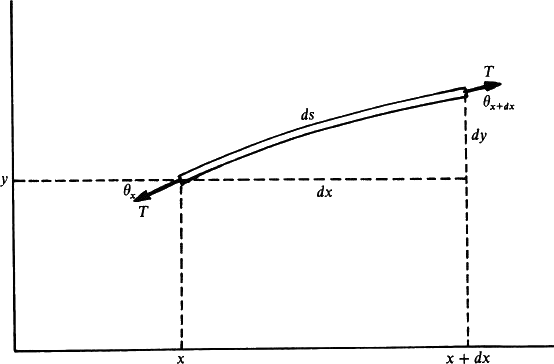
\includegraphics[width=0.65\linewidth]{00_Images/02_chapter/01.png}
    \caption{Forces on a differential string element under tension \(T\)}
    \label{fig:stringelement}
\end{figure}

Take a short string segment between \( x \) and \( x + dx \). The geometry and the force balance on the differential element are sketched in figure \ref{fig:stringelement}. The vertical components of the tension at the two ends are \( (T\sin\theta)_x \) and \( (T\sin\theta)_{x + dx} \). The net vertical force on the segment is therefore
\[
dF_y = (T\sin\theta)_{x + dx} - (T\sin\theta)_x
    = \frac{\partial(T\sin\theta)}{\partial x}dx
\]
For small transverse displacements, the slope is small and one may approximate
\[
\sin\theta \simeq \tan\theta = \frac{\partial y}{\partial x}
\]
so that
\[
dF_y = T\frac{\partial^2 y}{\partial x^2}dx
\]
Applying Newton's second law to the same element,
\[
dF_y = (\mu ds)\frac{\partial^2 y}{\partial t^2}
\]
and for small displacements \( ds\simeq dx \). Hence,
\[
T\frac{\partial^2 y}{\partial x^2}dx = \mu dx\frac{\partial^2 y}{\partial t^2}
\qquad\Longrightarrow\qquad
\frac{\partial^2 y}{\partial t^2} = c^2\frac{\partial^2 y}{\partial x^2}
\]
where the transverse wave speed is
\[
c = \sqrt{\frac{T}{\mu}}
\]
This is the one-dimensional wave equation for an ideal string (uniform tension, small slopes, no losses).

\subsection{Traveling-Wave Solution and Boundary Conditions}

The general solution of the wave equation can be written as the superposition of two traveling waves,
\[
y(x,t) = f_1(ct-x) + f_2(ct + x)
\]
where \( f_1 \) travels towards increasing \( x \) and \( f_2 \) travels towards decreasing \( x \), both with speed \( c \).
To determine the specific functions \( f_1 \) and \( f_2 \), two types of constraints are required:

\begin{itemize}
\item Initial conditions: the displacement \( y(x,0) \) and velocity \( \partial y/\partial t(x,0) \) must match the initial state produced by the excitation.
\item Boundary conditions: for a finite string, conditions must be satisfied at the endpoints (values of \( y \) or its spatial derivative).
\end{itemize}

Two idealized endpoint conditions are especially important. Assuming the end is located at \( x = 0 \):

\begin{itemize}
\item Fixed end: \( y(0,t) = 0 \). Then
\[
f_1(ct) + f_2(ct) = 0
\qquad\Longrightarrow\qquad
f_1(ct) = -f_2(ct)
\]
the reflected traveling wave is inverted in sign.
\item Free end: no transverse force can be exerted; hence \( \partial y/\partial x(0,t) = 0 \). Since
\[
\frac{\partial y}{\partial x} = -f_1'(ct-x) + f_2'(ct + x)
\]
at \( x = 0 \) one obtains
\[
-f_1'(ct) + f_2'(ct) = 0
\qquad\Longrightarrow\qquad
f_2'(ct) = f_1'(ct)
\]
Under the usual assumption of no energy creation at the boundary, this implies \( f_1(ct) = f_2(ct) \): the reflected wave is non-inverted.
\end{itemize}

\subsection{Harmonic Waves and Wavenumber}

Any complex waveform can be decomposed into (possibly infinitely many) sinusoidal components. Consider a single harmonic component at temporal angular frequency \( \omega \). A general real traveling-wave representation is
\[
y(x,t) = A\sin(\omega t-kx) + B\cos(\omega t-kx) + C\sin(\omega t + kx) + D\cos(\omega t + kx)
\]
where the wavenumber \( k \) is
\[
k = \frac{\omega}{c} = \frac{2\pi}{\lambda}
\]
and \( \lambda \) is the wavelength. It is often convenient to use the complex form,
\[
\widetilde{y}(x,t) = \widetilde{A}e^{j(\omega t-kx)} + \widetilde{B}e^{j(\omega t + kx)},
\qquad
y(x,t) = \Re\{\widetilde{y}(x,t)\}
\]
The arbitrary constants (either \( A,B,C,D \) or \( \widetilde{A},\widetilde{B} \) ) are determined by imposing initial and boundary conditions.

\subsection{Standing Waves and Normal Modes of a Fixed String}

Consider a string of length \( L \) fixed at both ends (\( x = 0 \) and \( x = L \)). The fixed-end conditions require
\[
y(0,t) = 0,\qquad y(L,t) = 0
\]
Imposing \( y(0,t) = 0 \) forces the left- and right-traveling components to combine into a standing wave form, which can be written as
\[
y(x,t) = 2\sin(kx)\left[A\cos(\omega t)-B\sin(\omega t)\right]
\]
Imposing the second boundary condition \( y(L,t) = 0 \) yields
\[
\sin(kL) = 0
\qquad\Longrightarrow\qquad
kL = n\pi,\quad n\in\mathbb{N}
\]
Using \( k = \omega/c \), the admissible (angular) frequencies are
\[
\omega_n = \frac{n\pi c}{L},
\qquad
k_n = \frac{n\pi}{L}
\]
The corresponding standing-wave patterns are the normal modes of the fixed string and a modal expansion of the motion may be written as
\[
y(x,t) = \sum_{n = 1}^{\infty}\left(A_n\sin(\omega_n t) + B_n\cos(\omega_n t)\right)\sin(k_n x)
\]
The constants \( A_n \) and \( B_n \) are set by the initial conditions, which in practice depend on the excitation mechanism (plucked, struck, bowed or externally driven).

\subsection{String Excitation Mechanisms: Plucked, Struck and Bowed}

The wave equation and its normal modes describe the admissible motions of an ideal string, but the actual vibration observed in an instrument depends crucially on how the motion is initiated and sustained. In this part we summarize three archetypal excitation mechanisms-plucking, striking and bowing-and show how they shape the modal amplitudes and the resulting spectrum.

\subsubsection{Plucked Strings: Modal Coefficients and Missing Harmonics}

When a string is plucked, the initial triangular displacement can be expanded in normal modes. Figure \ref{fig:pluckmodes} illustrates the modal distribution for a string plucked at midspan: by symmetry, even modes have vanishing participation while odd modes dominate the response.

\begin{figure}[!htb]
    \centering
    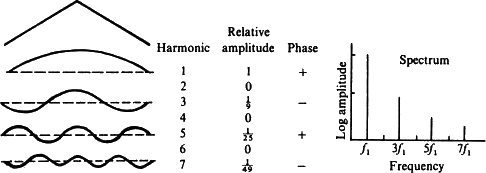
\includegraphics[width=0.9\linewidth]{00_Images/02_chapter/02.png}
    \caption{Modal participation for a string plucked at midspan}
    \label{fig:pluckmodes}
\end{figure}

For a string of length \( L \) fixed at both ends, the displacement can be expanded in normal modes as
\[
y(x,t) = \sum_{n = 1}^{\infty}\left[A_n\sin(\omega_n t) + B_n\cos(\omega_n t)\right]\sin\left(\frac{n\pi x}{L}\right),
\qquad
\omega_n = \frac{n\pi c}{L}
\]
The coefficients are determined by the initial conditions \( y(x,0) \) and \( \dot{y}(x,0) \) through orthogonality:
\[
A_n = \frac{2}{\omega_n L}\int_{0}^{L}\dot{y}(x,0)\sin\left(\frac{n\pi x}{L}\right)dx,
\qquad
B_n = \frac{2}{L}\int_{0}^{L}y(x,0)\sin\left(\frac{n\pi x}{L}\right)dx
\]
For an ideal pluck released from rest, one has \( \dot{y}(x,0) = 0 \), hence \( A_n = 0 \) and the spectrum is entirely determined by \( B_n \).

\paragraph{Pluck at the midpoint} Assume a triangular initial shape with maximum displacement \( h \) at \( x = L/2 \). The resulting coefficients take the form
\[
B_n = \frac{8h}{\pi^2 n^2}\sin\left(\frac{n\pi}{2}\right)
\]
Therefore all even modes are absent (since \( \sin(n\pi/2) = 0 \) for even \( n \) ), while the odd harmonics alternate in sign because \( \sin(n\pi/2) = \pm 1 \). This selection rule is a direct consequence of symmetry: even modes have a node at the midpoint and cannot reproduce a midpoint maximum at \( t = 0 \).

\paragraph{Pluck at a fraction of the length} Let the string be plucked at \( x = L/5 \) and released from rest with a triangular initial displacement of height \( h \). Then
\[
B_n = \frac{25h}{2\pi^2 n^2}\sin\left(\frac{n\pi}{5}\right),
\qquad
A_n = 0
\]
The factor \( \sin(n\pi/5) \) implies \( B_n = 0 \) for \( n = 5,10,15,\dots \): when the pluck point is at \( x = L/g \) with \( g\in\mathbb{N} \), the modes \( g,2g,3g,\dots \) are absent. In the time domain, the initial triangular shape may be interpreted as two sharp bends that propagate in opposite directions and reflect at the ends, generating the familiar periodic motion of a plucked string. 

\begin{figure}[!htb]
    \centering
    \subfloat[Evolution and the resulting boundary force]{
        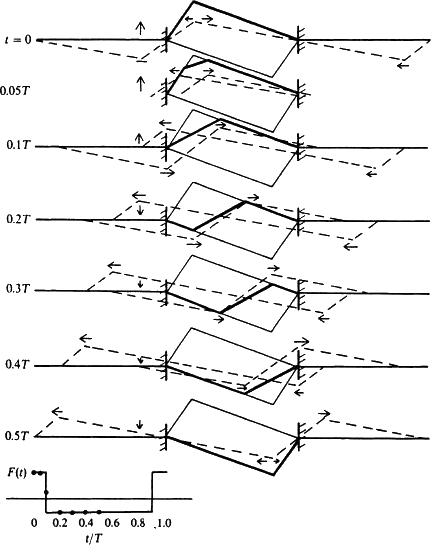
\includegraphics[width=0.45\linewidth]{00_Images/02_chapter/03.png}
    }
    \hfill
    \subfloat[Spectrum of the modes]{
        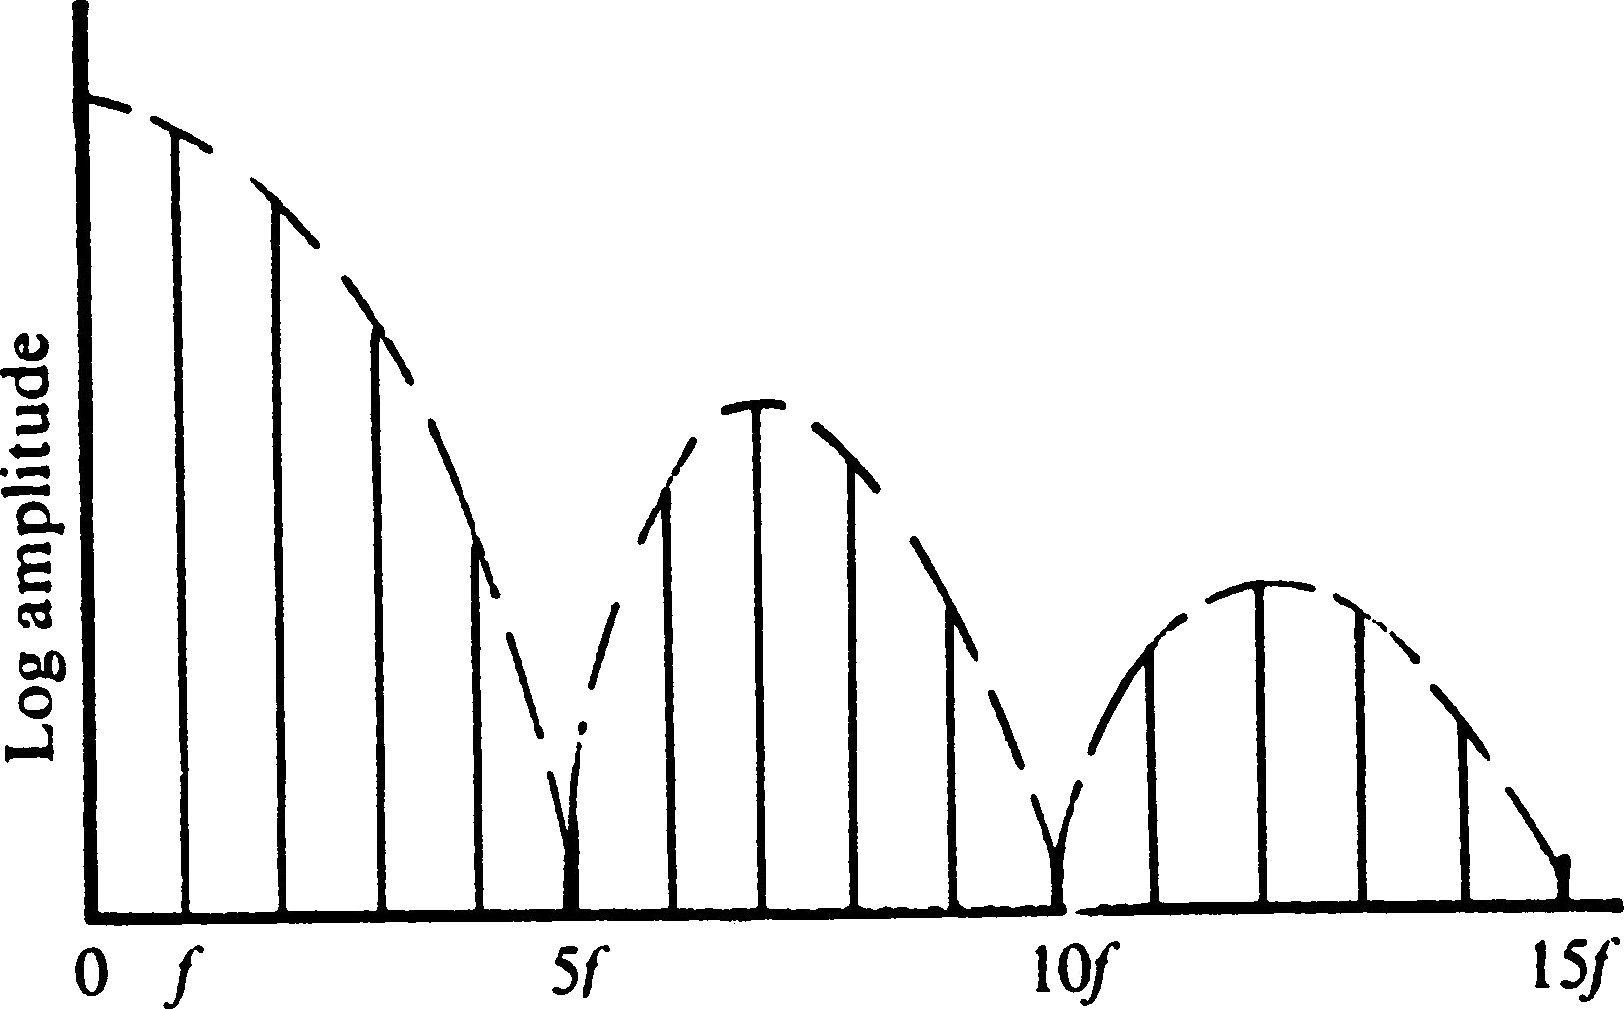
\includegraphics[width=0.45\linewidth]{00_Images/02_chapter/04.png}
    }
    \caption{Results for a string plucked at one-fifth of its total length}
    \label{fig:pluckevolution}
\end{figure}

\subsubsection{Struck Strings: Hammer Interaction and Spectral Envelope}

In a struck string, the excitation is mediated by a hammer of finite mass \( M \) impacting the string at \( x = x_0 \) with initial velocity \( V \). As time increases, the disturbance spreads along the string: after a time \( t \) the portion of string involved in the motion has length \( 2ct \) and mass \( 2\mu ct \). As this effective moving mass becomes comparable with \( M \), the hammer is progressively slowed down. At the contact point, the force exerted by the hammer must be balanced by the restoring force associated with the string tension. This can be expressed by writing Newton's law for the hammer in terms of the discontinuity of the string slope at the impact point,
\[
M\frac{\partial^2 y}{\partial t^2}(x_0,t) = T\Delta\left(\frac{\partial y}{\partial x}\right)
\]
where \( \Delta(\partial y/\partial x) \) denotes the jump in slope across \( x_0 \). Solving this interaction problem (before any reflected waves return to the contact point) yields an exponentially decaying contact velocity
\[
v(x_0,t) = V e^{-t/\tau},
\qquad
\tau = \frac{Mc}{2T}
\]
and the corresponding contact displacement
\[
y(x_0,t) = V\tau\left(1-e^{-t/\tau}\right)
\]
For a finite string, reflections from the endpoints eventually return to \( x_0 \) and can throw the hammer off the string before it comes fully to rest; after separation, the string vibrates freely in its normal modes.

\paragraph{Spectral consequences} Compared with plucking (where modal amplitudes typically scale as \( 1/n^2 \) ), striking produces a much richer high-frequency content. In the limit \( M\ll M_s \) (string mass \( M_s \) ), the displacement spectrum exhibits dips to zero at harmonic numbers that are multiples of \( 1/\beta \) when the string is struck at a fraction \( \beta \) of its length, while remaining otherwise relatively flat. If \( M \) is small but not negligible, the spectrum is approximately constant up to a mode number
\[
n_m \simeq 0.73\frac{M_s}{M}
\]
and above \( n_m \) it falls off as \( 1/n \), i.e. much more slowly than for plucking. The traveling velocity pulses that initiate this response are illustrated in figure \ref{fig:struckpulses}.

\begin{figure}[!htb]
    \centering
    
\includegraphics[width=0.9\linewidth]{00_Images/02_chapter/05.png}
    \caption{Velocity pulses generated by striking a string}
    \label{fig:struckpulses}
\end{figure}

\subsubsection{Bowed Strings: Helmholtz Motion and Stick-Slip Energy Input}

The bowed string is not merely an initial-value problem: the bow continuously injects energy into the string through friction at the contact point. The ideal periodic motion of a bowed string is known as Helmholtz motion. Kinematically, the string waveform is approximately triangular, with a single sharp bend (a traveling ``corner'') that runs back and forth along the string. At a fixed observation point, the velocity waveform alternates between two values, reflecting the alternation between two dynamical regimes. The characteristic waveform and the associated stick-slip cycle are summarized in figure \ref{fig:helmholtz_stickslip}.

\begin{figure}[!htb]
    \centering
    \subfloat[Helmholtz waveform and velocity at different positions]{
        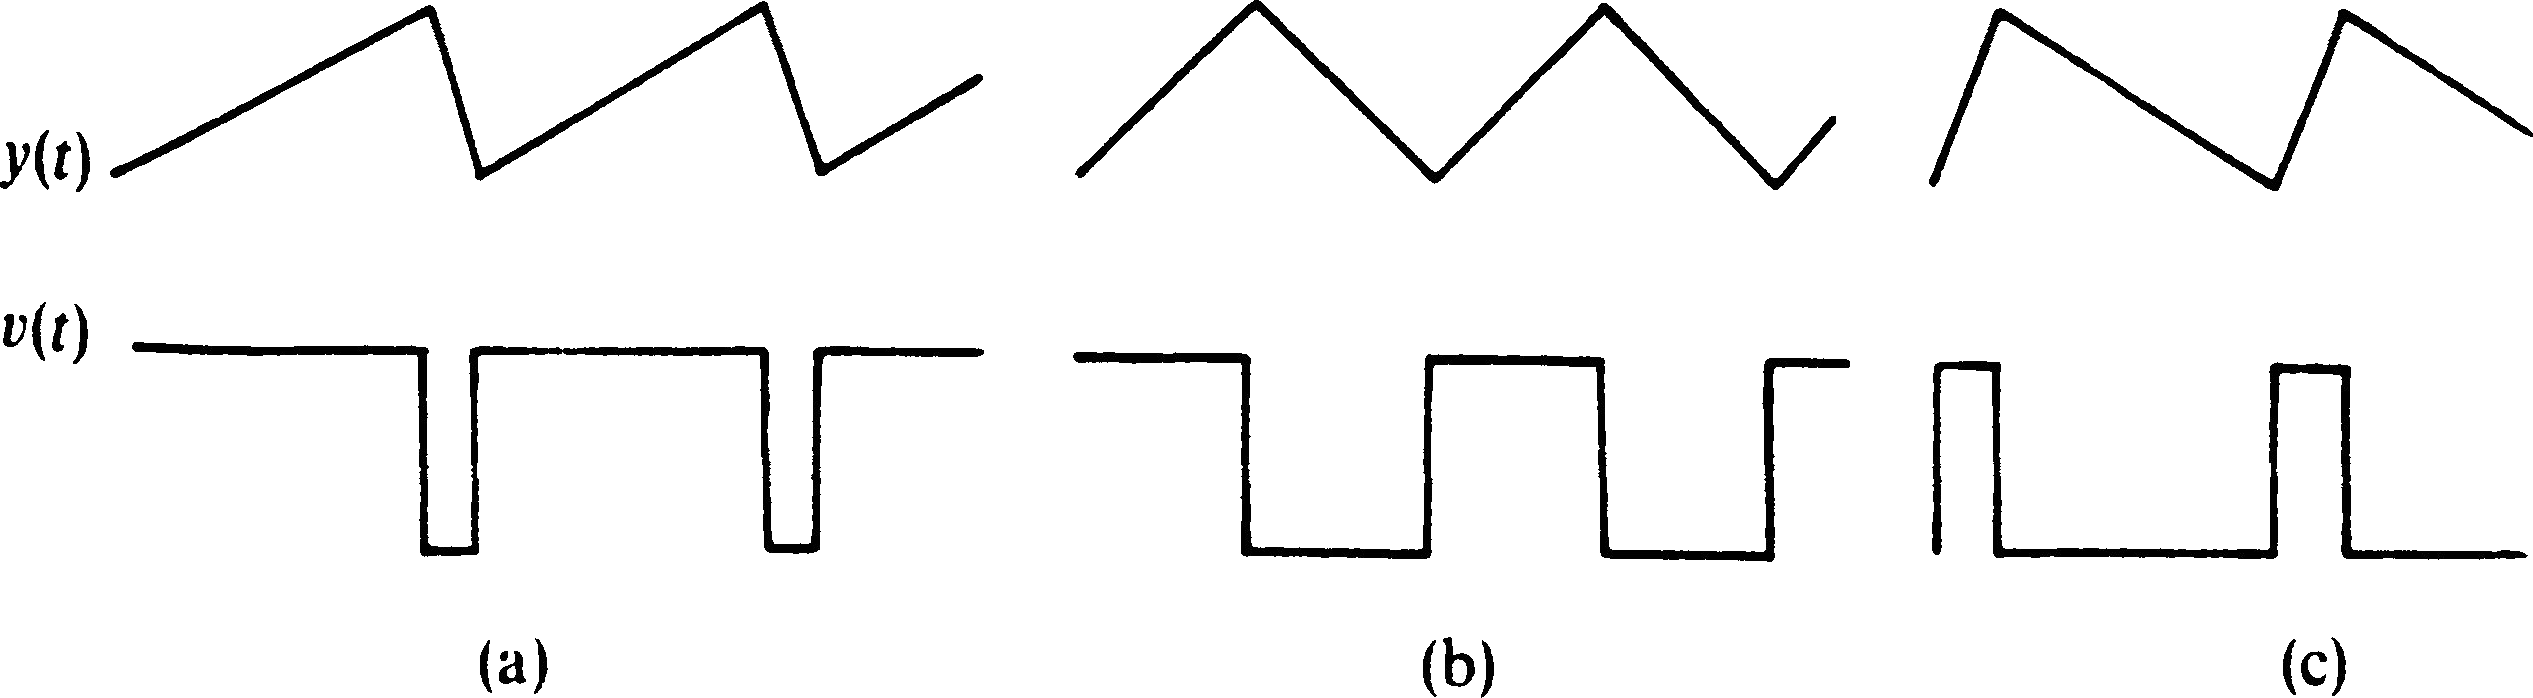
\includegraphics[width=0.48\linewidth]{00_Images/02_chapter/06.png}
    }\hfill
    \subfloat[Stick-slip cycle at the bowing point]{
        
\includegraphics[width=0.48\linewidth]{00_Images/02_chapter/07.png}
    }
    \caption{Helmholtz motion in a bowed string and the corresponding stick-slip mechanism}
    \label{fig:helmholtz_stickslip}
\end{figure}

\paragraph{Stick-slip mechanism} During part of the cycle the bow hair drags the string (stick phase): bow and string move in the same direction and static friction dominates. When the traveling bend arrives at the bowing point, the string suddenly releases (slip phase): bow and string move in opposite directions and dynamic friction dominates. Since the frictional force is higher during the stick phase, the net energy transfer over a full cycle is from the bow to the string, compensating internal and radiation losses and sustaining steady oscillation.

\paragraph{Comparison with plucking} A plucked string can be interpreted as two counter propagating bends (two traveling discontinuities), while the ideal bowed string exhibits a single traveling bend. This difference is reflected in the time waveform and in the harmonic content: the near piecewise-linear displacement and piecewise-constant velocity of Helmholtz motion naturally support a strong harmonic series, consistent with the bright timbre of bowed-string instruments.

\subsection{Input Impedance of a String}

\paragraph{Semi-Infinite String} Consider a string driven at \( x = 0 \) by a harmonic force
\[
e_f(t) = F e^{j\omega t}
\]
Assume first an infinitely long string, so that no reflected wave is present: only a forward-traveling wave propagating towards increasing \( x \) can exist,
\[
y_e(x,t) = A e^{j(\omega t-kx)}
\]
At the driving point, the applied force must be balanced by the vertical component of the string tension. Under small-slope assumptions,
\[
F e^{j\omega t} = -T\left.\frac{\partial y_e}{\partial x}\right|_{x = 0}
\]
Since \( \partial y_e/\partial x = -jkA e^{j(\omega t-kx)} \), at \( x = 0 \) this gives
\[
F e^{j\omega t} = jkT A e^{j\omega t}
\qquad\Longrightarrow\qquad
A = -j\frac{F}{kT}
\]
The transverse velocity follows from time differentiation:
\[
u_e(x,t) = \frac{\partial y_e}{\partial t}
 = j\omega A e^{j(\omega t-kx)}
 = \frac{F\omega}{kT}e^{j(\omega t-kx)}
\]
The input impedance (driving-point impedance) is defined as the ratio of force to velocity at the driving point,
\[
Z_{\mathrm{in}} = \left.\frac{\text{Force}}{\text{Velocity}}\right|_{x = 0}
 = \frac{F e^{j\omega t}}{u_e(0,t)}
 = \frac{kT}{\omega}
 = \frac{T}{c},
\qquad c = \frac{\omega}{k}
\]
Hence, the input impedance of an infinite string is purely resistive and constant: it does not depend on frequency or on the position where the string is driven.

\paragraph{Finite String} Now consider a finite string of length \( L \), fixed at the far end:
\[
y_e(L,t) = 0
\]
Because of reflection at \( x = L \), the motion is a superposition of forward and backward traveling waves,
\[
y_e(x,t) = A e^{j(\omega t-kx)} + B e^{j(\omega t + kx)}
\]
Imposing the boundary condition at \( x = L \) yields
\[
A e^{-jkL} + B e^{jkL} = 0
\qquad\Longrightarrow\qquad
B = -A e^{-j2kL}
\]
The driving condition at \( x = 0 \) is again force balance,
\[
F e^{j\omega t} = -T\left.\frac{\partial y_e}{\partial x}\right|_{x = 0}
\]
Solving the two conditions gives the string motion in the compact standing-wave form
\[
y_e(x,t) = \frac{F}{kT}\frac{\sin[k(L-x)]}{\cos(kL)}e^{j\omega t}
\]
and the corresponding velocity
\[
u_e(x,t) = \frac{\partial y_e}{\partial t}
 = j\omega\frac{F}{kT}\frac{\sin[k(L-x)]}{\cos(kL)}e^{j\omega t}
\]
Evaluating at the driving point \( x = 0 \), the input impedance becomes
\[
Z_{\mathrm{in}}
 = \left.\frac{F e^{j\omega t}}{u_e(x,t)}\right|_{x = 0}
 = -\frac{jkT}{\omega}\frac{\cos(kL)}{\sin(kL)}
 = -\frac{jkT}{\omega}\cot(kL)
\]
Therefore, for an ideal lossless finite string fixed at the end, the input impedance is purely reactive: force and velocity are in quadrature (shifted by \( 90^\circ \) ). Moreover,
\[
|Z_{\mathrm{in}}| \to \infty \quad \text{when } kL = 0,\pi,2\pi,\dots
\qquad\text{and}\qquad
Z_{\mathrm{in}} \to 0 \quad \text{when } kL = \frac{\pi}{2},\frac{3\pi}{2},\dots
\]
corresponding respectively to impedance maxima (near modal resonances) and minima (quarter-wave conditions).

\subsection{Nonideal Ends: Mass Loading at the Termination}

The ideal fixed-end condition \( y(L,t) = 0 \) corresponds to an infinite termination impedance. In real instruments, the string end is attached to a bridge of finite effective mass, so the boundary is neither perfectly fixed nor perfectly free. A simple and useful model consists of a string fixed at \( x = 0 \) and terminated at \( x = L \) by a lumped mass \( m \), representing a lightweight bridge. Assume harmonic motion and write the string displacement as a superposition of traveling waves,
\[
y_e(x,t) = A e^{j(\omega t-kx)} + B e^{j(\omega t + kx)}
\]
The boundary condition at the fixed end \( x = 0 \) imposes
\[
y_e(0,t) = 0 \quad\Longrightarrow\quad A + B = 0 \quad\Longrightarrow\quad B = -A
\]
so that the motion can be written in standing-wave form,
\[
y_e(x,t) = A\sin(kx)e^{j\omega t}
\]
At the termination \( x = L \), Newton's second law regarding the attached mass requires that the transverse force transmitted by the string equals the inertial force of the mass:
\[
-T\left.\frac{\partial y_e}{\partial x}\right|_{x = L} = m\left.\frac{\partial^2 y_e}{\partial t^2}\right|_{x = L}
\]
Using \( \partial y_e/\partial x = Ak\cos(kx)e^{j\omega t} \) and \( \partial^2 y_e/\partial t^2 = -\omega^2 A\sin(kx)e^{j\omega t} \), one obtains
\[
-TAk\cos(kL)e^{j\omega t} = -m\omega^2A\sin(kL)e^{j\omega t}
\quad\Longrightarrow\quad
\cot(kL) = \frac{\omega^2 m}{kT}
\]
Since \( \omega = ck \) and \( c^2 = T/\mu \), defining the string mass \( M = \mu L \) provides the compact transcendental condition
\[
\cot(kL) = \frac{m}{M}kL
\]
The admissible wavenumbers \( k \) (and thus the natural frequencies \( \omega = ck \) ) are the intersections between \( \cot(kL) \) and the straight line \( \frac{m}{M}kL \); there is no closed-form solution in general, so a graphical (or numerical) root-finding approach is used. This graphical construction is shown in figure \ref{fig:massloaded_roots}.

\begin{figure}[!htb]
    \centering
    
\includegraphics[width=0.65\linewidth]{00_Images/02_chapter/08.png}
    \caption{Graphical solution of \( \cot(kL) = \frac{m}{M}kL \) for a mass-loaded termination}
    \label{fig:massloaded_roots}
\end{figure}

\paragraph{Frequency compression and loss of harmonicity} When \( m \gg M \), the straight line is steep and the roots approach \( kL = n\pi \), recovering the modes of a string with effectively fixed ends. When \( m \) and \( M \) are comparable, the roots are shifted so that the resonance frequencies are no longer equally spaced: the harmonic relationship is lost and the spacing between successive resonances is compressed with respect to the ideal fixed-end case. This compression is most visible for the lowest modes and becomes less pronounced at higher mode numbers, for which the spacing tends towards an approximately constant value. 


\subsection{Damping in Strings}

Ideal strings are lossless and would vibrate forever. Real strings, instead, show an approximately exponential decay of the motion amplitude, caused by several dissipation mechanisms. In practice, three main contributions are typically distinguished:

\begin{enumerate}
    \item interaction of the string with the surrounding air;
    \item internal losses in the string material;
    \item transfer of energy from the string to other coupled systems (supports, bridge, soundboard).
\end{enumerate}

Each mechanism produces an exponential envelope with its own characteristic decay time and their effects combine into an overall decay rate. Typical trends of the three decay times and their frequency dependence are summarized in figure \ref{fig:string_damping_regimes}.

\begin{figure}[!htb]
    \centering
    
\includegraphics[width=0.65\linewidth]{00_Images/02_chapter/09.png}
    \caption{Typical decay-time regimes for air, internal, and support losses in strings}
    \label{fig:string_damping_regimes}
\end{figure}

\paragraph{Air Losses} During vibration the string drags some air. This has two observable consequences: an added effective mass that slightly lowers the modal frequencies and a resistive force roughly proportional to the transverse velocity, leading to an exponential decay. For a cylindrical string of radius \( r \) and length \( L \), moving at velocity amplitude \( v \) at frequency \( f \), the air resistance force may be written as
\[
F_r
 = 
2\pi\rho_a f v r^2
\left(
\frac{\sqrt{2}}{M}
 + \frac{1}{2M^2}
\right),
\qquad
M = \frac{r}{2}\sqrt{\frac{2\pi f}{\eta_a}}
\]
where \( \rho_a \) is air density and \( \eta_a \simeq \SI{1.5e-5}{\meter\squared\per\second} \) is the kinematic viscosity of air.
Because \( F_r\propto v \), the motion magnitude decays exponentially with a decay time of the form
\[
\tau_1 = 
\frac{\rho}{2\pi\rho_a f}
\left(
\frac{2M^2}{2\sqrt{2}M + 1}
\right)
\]
In particular, the scaling transitions between
\[
\tau_1 \propto \rho r^2 \quad \text{(low frequency)},
\qquad
\tau_1 \propto \frac{\rho r}{\sqrt{f}} \quad \text{(high frequency)}
\]

\paragraph{Internal Losses} String materials are not perfectly elastic: when a force is applied, strain does not follow instantaneously, implying a viscoelastic behavior. A convenient model accounts for this by introducing a complex Young modulus
\[
E = E_r + j E_i
\]
where \( E_i \) represents the loss component and typically shows a peak around a relaxation frequency \( \omega\simeq 1/\tau \). Substituting the complex modulus into the equation of motion leads again to an exponential decay of the oscillation magnitude, with decay time
\[
\tau_2 = \frac{1}{\pi f}\frac{E_r}{E_i}
\]
Typical values for the ratio \( E_r/E_i \) span a wide range (from \( 10^{-5} \) to \( 10^{-1} \) ), hence internal damping can vary dramatically across materials (steel vs gut/nylon) and frequency ranges. 

\paragraph{Energy Transfer to Supports} When the string is attached to a lightweight bridge, a significant fraction of its vibrational energy can be transmitted to the end supports (bridge and instrument body). This mechanism is naturally described in terms of the mechanical admittance \( G \) (inverse of the impedance) presented by the termination. For mode \( n \), the velocity amplitude may be expressed as a linear relationship of the form
\[
v_n = \alpha GF_n
\]
where \( \alpha \) is a constant and \( F_n \) is the modal force. This implies a first-order dissipative term and therefore an exponential decay with decay time
\[
\tau_3 = \frac{1}{8\mu L f^{2}G}
\]
This contribution becomes increasingly important at higher frequency because it scales as \( 1/f^2 \).

\paragraph{Combined Effect and Typical Regimes} Since the mechanisms act approximately independently on the decay rate, the overall decay time \( \tau \) is well approximated by
\[
\frac{1}{\tau} = \frac{1}{\tau_1} + \frac{1}{\tau_2} + \frac{1}{\tau_3}
\]
Three limiting regimes are often observed:

\begin{itemize}
    \item thin metal strings: air damping dominates, giving roughly \( \tau \propto 1/\sqrt{f} \), hence relatively small attenuation of high partials (brilliant sound);
    \item gut or nylon strings: internal losses dominate, giving \( \tau \propto 1/f \), hence stronger relative damping of upper partials (less brilliant timbre);
    \item lightweight bridge / strong end losses: support losses dominate, giving \( \tau \propto 1/f^{2} \), strongly suppressing high-frequency components.
\end{itemize}

\section{Bars: Longitudinal and Bending Vibrations}

Unlike an ideal string, a bar is a stiff one-dimensional structure: besides transverse motion, it can sustain longitudinal (compressional) waves and, most importantly for many idiophones and structural elements, flexural (bending) waves. These wave types are governed by different PDEs, have different propagation laws and generally lead to modal frequencies that are not harmonically spaced. 

\subsection{Longitudinal Vibrations in a Bar}

\begin{figure}[!htb]
    \centering
    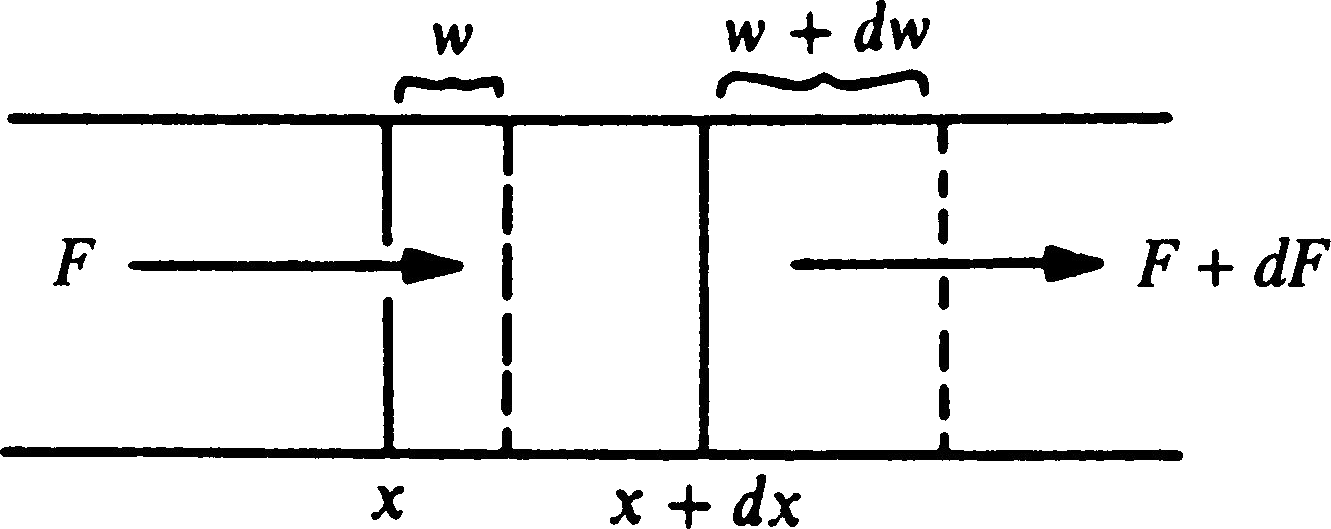
\includegraphics[width=0.55\linewidth]{00_Images/02_chapter/10.png}
    \caption{Forces and displacement of a differential bar element in longitudinal motion}
    \label{fig:bar_element_longitudinal}
\end{figure}

Consider a short bar element of length \( dx \), cross-sectional area \( S \), density \( \rho \)  and Young modulus \( E \) (figure \ref{fig:bar_element_longitudinal}). Let \( w(x,t) \) be the longitudinal displacement of the cross section at position \( x \). The longitudinal strain is
\[
\varepsilon(x,t) = \frac{\partial w}{\partial x}
\]
and Hooke's law relates stress and strain as \( \sigma = E\varepsilon \). Since \( \sigma = F/S \), one obtains
\[
F(x,t) = SE\frac{\partial w}{\partial x}
\]
Expanding \( F(x + dx,t) \) to first order gives
\[
dF = F(x + dx,t)-F(x,t) = \frac{\partial F}{\partial x}dx
   = SE\frac{\partial^2 w}{\partial x^2}dx
\]
The mass of the element is \( \rho Sdx \), hence Newton's law yields
\[
dF = \rho Sdx\frac{\partial^2 w}{\partial t^2}
\]
Combining the two relations gives the 1D longitudinal wave equation
\[
\frac{\partial^2 w}{\partial t^2}
 = 
\frac{E}{\rho}\frac{\partial^2 w}{\partial x^2}
\]
with longitudinal wave speed
\[
c_L = \sqrt{\frac{E}{\rho}}
\]
The structure of this equation is identical to the transverse-string wave equation, but the wave speed is now set by material parameters, not by tension. As a consequence, longitudinal waves also exist in stiff strings and their resonance frequencies are generally not in harmonic relation with the transverse ones. 

\paragraph{Mode frequencies} For a bar of length \( L \), the end conditions determine the standing waves. In particular:
\[
f_n = \frac{nc_L}{2L},\qquad n = 1,2,3,\dots
\]
for both ends fixed or both ends free, while for a bar fixed at one end and free at the other,
\[
f_m = \frac{mc_L}{4L},\qquad m = 1,3,5,\dots
\]
as in the standard quarter-wave pattern.

\subsection{Bending Waves in a Thin Bar (Flexural Waves)}

Bars also support transverse motion \( y(x,t) \) due to bending. In the thin-bar (Euler-Bernoulli) approximation, the transverse dynamics are governed by a fourth-order PDE, which may be written as
\[
\frac{\partial^2 y}{\partial t^2}
 = 
-\frac{E K^2}{\rho}\frac{\partial^4 y}{\partial x^4}
\]
Here \( K \) is the radius of gyration of the cross section,
\[
K^2 = \frac{1}{S}\int z^2dS
\]
where \( z \) is the distance from the neutral axis and \( S \) is the cross-sectional area. Figure \ref{fig:gyration_radius} illustrates the radius of gyration for typical cross-sectional shapes.

\begin{figure}[!htb]
    \centering
    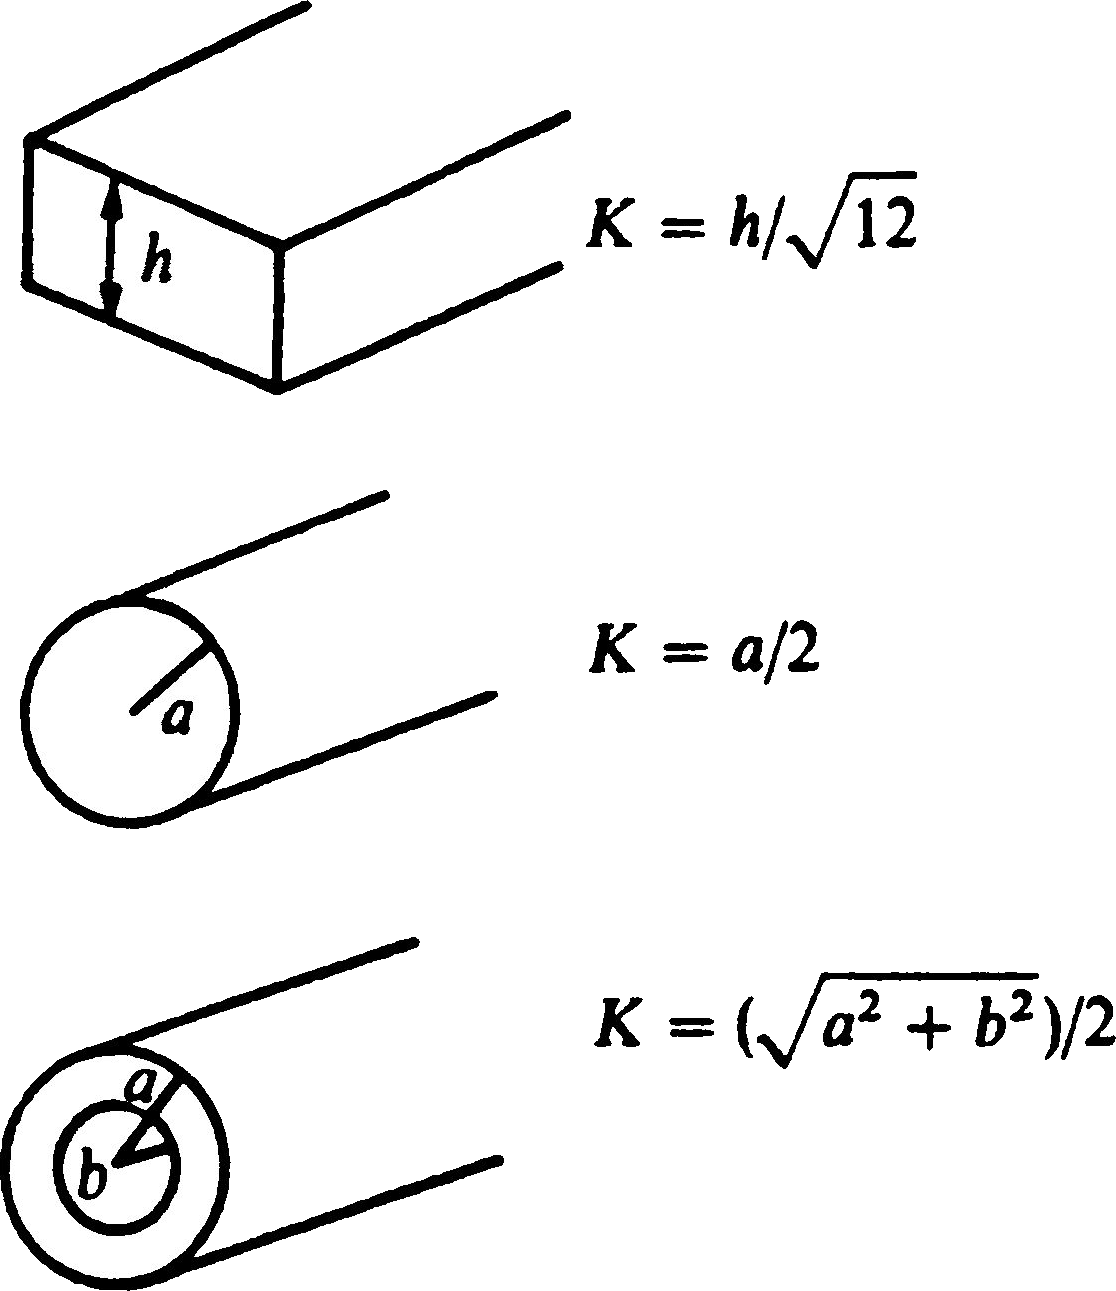
\includegraphics[width=0.5\linewidth]{00_Images/02_chapter/11.png}
    \caption{Radius of gyration \(K\) for typical bar cross sections}
    \label{fig:gyration_radius}
\end{figure}

\paragraph{Dispersion and propagation number} Because a fourth spatial derivative appears, flexural waves are dispersive: different frequency components propagate at different speeds. Introducing a separable harmonic solution
\[
y_e(x,t) = Y_e(x)e^{-j\omega t}
\]
and substituting gives
\[
\frac{d^4 Y_e}{dx^4} = \frac{\rho\omega^2}{E K^2}Y_e
\]
Defining the propagation number \( k \) through
\[
k^4 = \frac{\rho\omega^2}{E K^2}
\]
one finds the dispersion relation
\[
\omega = K\sqrt{\frac{E}{\rho}}k^2
\qquad
v_p = \frac{\omega}{k}
 = \left(K\sqrt{\frac{E}{\rho}}\right)k
\propto \sqrt{\omega}
\]
so the phase speed increases with frequency. 

\paragraph{General harmonic solution} Seeking exponential solutions \( Y_e(x) = Ae^{\gamma x} \) gives \( \gamma^4 = k^4 \), hence
\[
\gamma = \pm k,\qquad \gamma = \pm jk
\]
Therefore, the general harmonic motion in a thin bar can be written as
\[
y_e(x,t) = e^{j\omega t}\left(Ae^{kx} + Be^{-kx} + Ce^{jkx} + De^{-jkx}\right)
\]
and the constants are determined by the boundary conditions at the ends.

\subsection{End Supports and Modal Frequencies in a Thin Bar}

For flexural motion, endpoint conditions involve both displacement and derivatives, because bending moment and shear force depend on curvature and its derivative. Three idealized supports are commonly used:

\begin{itemize}
\item Free end: no bending moment and no shear force,
\[
\left.\frac{\partial^2 y}{\partial x^2}\right|_{\text{end}} = 0,
\qquad
\left.\frac{\partial^3 y}{\partial x^3}\right|_{\text{end}} = 0.
\]
\item Supported end (simply supported): zero displacement and no bending moment,
\[
\left.y\right|_{\text{end}} = 0,
\qquad
\left.\frac{\partial^2 y}{\partial x^2}\right|_{\text{end}} = 0.
\]
\item Clamped end: zero displacement and zero slope,
\[
\left.y\right|_{\text{end}} = 0,
\qquad
\left.\frac{\partial y}{\partial x}\right|_{\text{end}} = 0.
\]
\end{itemize}

Figure \ref{fig:diffendbar} summarizes what is written above and figure \ref{fig:barmodeshapes} shows the corresponding normal-mode shapes and relative modal frequencies for the most common end conditions described after.

\begin{figure}[!htb]
    \centering
    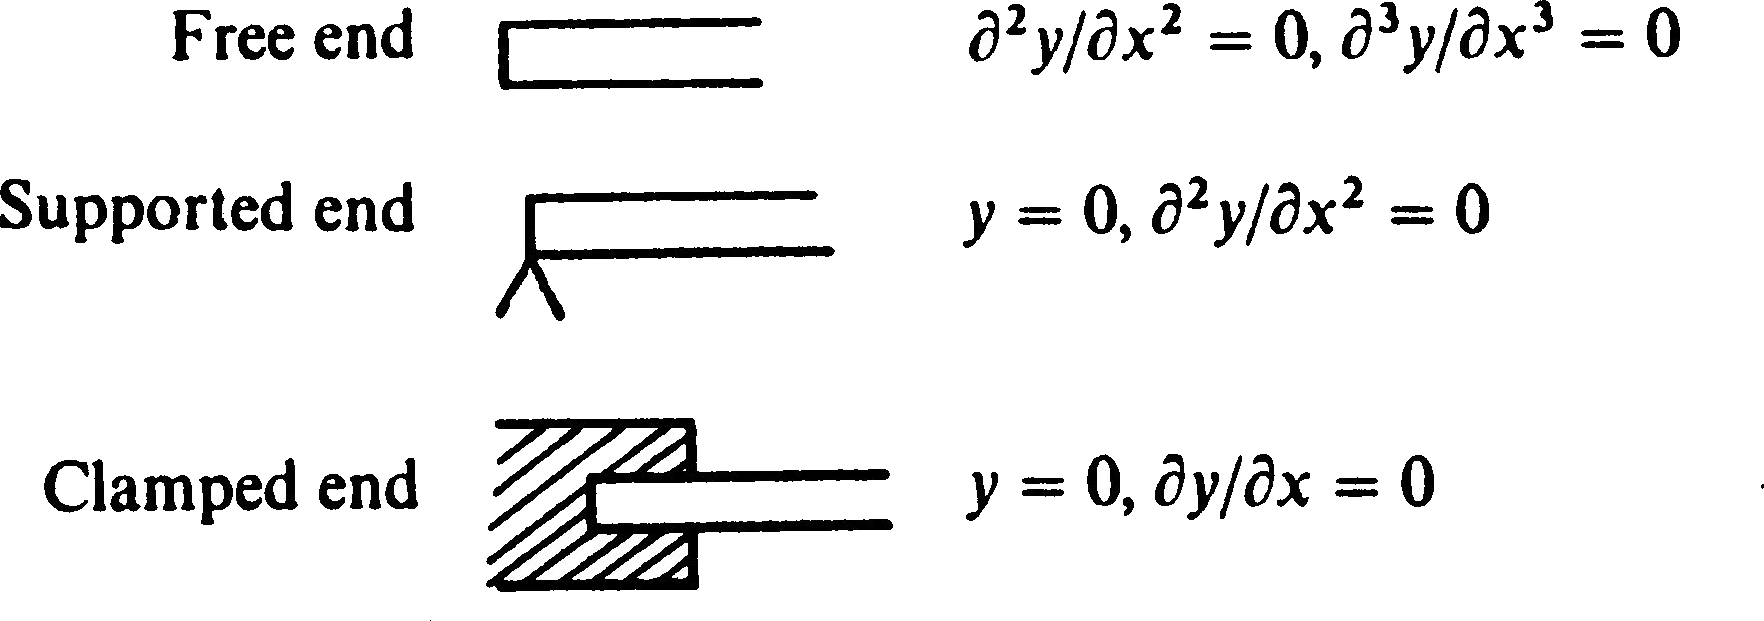
\includegraphics[width=0.65\linewidth]{00_Images/02_chapter/12.png}
    \caption{Idealized boundary conditions for flexural vibration: free, simply supported, and clamped ends}
    \label{fig:diffendbar}
\end{figure}

\begin{figure}[!htb]
    \centering
    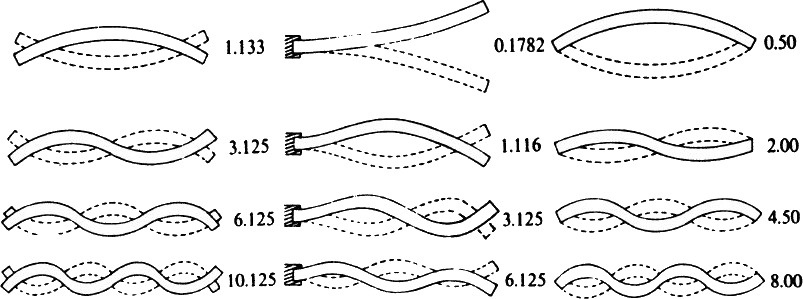
\includegraphics[width=0.85\linewidth]{00_Images/02_chapter/13.png}
    \caption{Normal modes of a bar for typical end conditions and their relative frequencies}
    \label{fig:barmodeshapes}
\end{figure}


\paragraph{Free-free bar} For a bar of length \( L \) free at both ends, the boundary conditions lead to the transcendental equation
\[
\tan\left(\frac{kL}{2}\right) = \pm\tanh\left(\frac{kL}{2}\right)
\]
whose roots yield the flexural modal frequencies in the form
\[
f_n = \frac{\pi K}{8L^2}\sqrt{\frac{E}{\rho}}
\beta_n^2,
\qquad
\beta_n\approx \left[3.011, 5, 7,\dots,(2n + 1)\right]
\]
The spacing is not harmonic and the departure from harmonicity is a direct consequence of dispersion.

\paragraph{Clamped-free bar (cantilever)} For a cantilevered bar (clamped at \( x = 0 \), free at \( x = L \) ), the characteristic condition becomes
\[
\cot\left(\frac{kL}{2}\right) = \pm\tanh\left(\frac{kL}{2}\right)
\]
leading to
\[
f_n = \frac{\pi K}{8L^2}\sqrt{\frac{E}{\rho}}
\beta_n^2,
\qquad
\beta_n\approx \left[1.1194, 2.988, 5, 7, \dots, (2n-1)\right]
\]
with frequencies lower than the free-free case. 

\paragraph{Supported-supported bar} For a bar supported at both ends, the modal frequencies reduce to the simple quadratic law
\[
f_m = \frac{\pi K}{2L^2}\sqrt{\frac{E}{\rho}}m^2,
\qquad
m = 1,2,3,\dots
\]
again emphasizing the non-harmonic pattern typical of flexural modes.

\section{Vibrations in Stiff Strings}

The ideal string model assumes that the restoring force is provided only by the string tension. In many practical cases (notably metallic strings), stiffness is not negligible and contributes an additional restoring action. The resulting dynamics combine the tension-driven wave equation with a bending (flexural) term, so the string becomes dispersive and its partials are no longer exactly harmonic.

\subsection{Equation of Motion and Dispersion Relation}

Let \( y(x,t) \) be the transverse displacement, \( T \) the tension and \( \mu \) the linear mass density. Including stiffness effects leads to the modified PDE
\[
\frac{\partial^{2}y}{\partial t^{2}}
 = 
c^{2}\frac{\partial^{2}y}{\partial x^{2}}
-\frac{ESK^{2}}{\mu}\frac{\partial^{4}y}{\partial x^{4}}
\]
where \( E \) is Young's modulus, \( S \) is the cross-sectional area and \( K \) is the radius of gyration of the cross section. Although does not generally admit a simple closed-form solution, useful insight follows from a traveling-wave ansatz
\[
y(x,t) = e^{j(\omega t-kx)}
\]
Substitution yields the dispersion equation
\[
\omega^{2} = k^{2}c^{2}\left(1 + \frac{EI}{T}k^{2}\right)
\]
where \( I \) is the second moment of area of the cross section. In particular, higher \( k \) (shorter wavelength) components have larger phase speed, which is the hallmark of dispersion, hence waveforms deform as they propagate.

\subsection{Normal Modes and Inharmonicity}

Introducing the dimensionless parameter
\[
\epsilon = \frac{EI}{TL^{2}}
\]
the dispersion relation may be rewritten as
\[
\omega^{2} = k^{2}c^{2}\left(1 + \epsilon k^{2}L^{2}\right)
\]
For a stiff string with supported (hinged) ends, the displacement and bending moment vanish at \( x = 0 \) and \( x = L \), leading to the wavenumber condition
\[
\sin(kL) = 0
\quad\Longleftrightarrow\quad
k_nL = n\pi
\]
The corresponding natural frequencies can be expressed as
\[
f_n = n f_1^{\circ}\sqrt{1 + Bn^{2}},
\qquad
B = \frac{\pi ESK^{2}}{TL^{2}}
\]
where \( f_1^{\circ} \) is the fundamental frequency of the same string in the ideal (tension-only) model. 

\paragraph{Discussion} The factor \( \sqrt{1 + Bn^{2}} \) shows that stiffness increases the frequencies with respect to the ideal string and the effect grows with mode number \( n \): high partials are stretched upward. Consequently, the partials are not in an exact harmonic relationship with the fundamental.

\subsection{Clamped Ends and Further Frequency Shifts}

If the ends are clamped rather than supported, the natural frequencies are further increased. A commonly used approximation is
\[
f_n
 = 
n f_1^{\circ}\sqrt{1 + Bn^{2}\left[1 + \frac{2}{\pi}B^{1/2} + \left(\frac{4}{\pi^{2}}\right)B\right]}
\]
In this case the end constraints stiffen the boundary, raising the modal frequencies. The stretching of the partials is present but may be slightly reduced in relative terms compared to the supported-end case. 

\subsection{Relevant Musical Cases}

\paragraph{Piano strings} For the lower piano strings, stiffness would cause overtones to deviate from harmonic tuning with the fundamentals of the upper strings. In practice, tuning compensates by stretching octaves slightly above the ideal \( 2:1 \) ratio. For example, the 4th harmonic of C4 may be a few cents sharp and the same harmonic for C5 even more so.

\paragraph{Violin strings} Metal violin strings also exhibit non-negligible stiffness. Dispersion implies that sharp bends in the bowed-string waveform do not propagate rigidly: the corner is sharp near the bow position but becomes progressively rounded while it travels freely, until it reaches the bow again.

\section{Dispersion: Phase and Group Velocity}

For an ideal (tension-only) string, the dispersion relation is linear,
\[
\omega = ck,
\qquad c = \sqrt{\frac{T}{\mu}}
\]
so all frequency components propagate with the same speed and a traveling waveform preserves its shape. Whenever the relation \( \omega(k) \) is not a straight line, the medium is dispersive: different wavenumbers travel differently and waveforms deform as they propagate. Two important cases in musical acoustics are stiff strings and strings loaded with discrete masses. Representative dispersion relations for these cases are compared in figure \ref{fig:dispersion_examples}.

\begin{figure}[!htb]
    \centering
    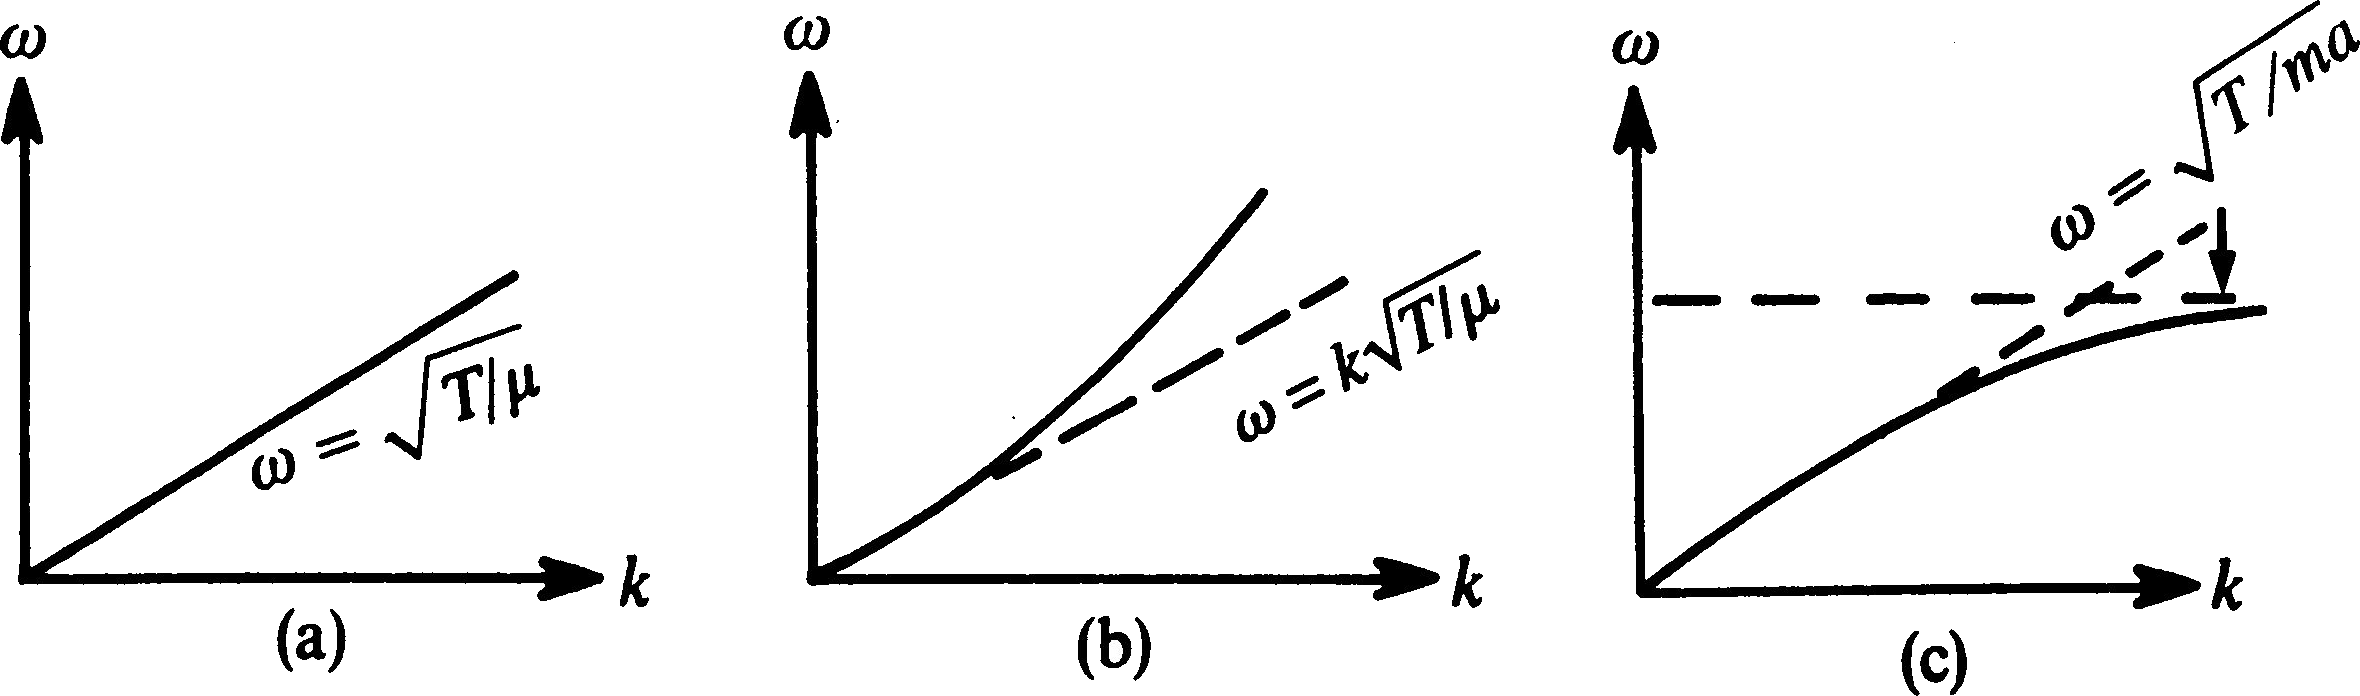
\includegraphics[width=0.9\linewidth]{00_Images/02_chapter/14.png}
    \caption{Dispersion relations for ideal, stiff, and mass-loaded strings}
    \label{fig:dispersion_examples}
\end{figure}

\subsection{Dispersion in Stiff Strings}

For a string with non-negligible stiffness (hinged ends), the natural frequencies can be expressed as
\[
\omega_n
 = 
n k_s \sqrt{\frac{T}{\mu}}\sqrt{1 + Bn^{2}}
 = 
n k_s \sqrt{\frac{T}{\mu}}\sqrt{1 + \alpha k^{2}}
\]
showing explicitly that the dependence on \( k \) (or on mode number \( n \) ) is no longer linear. As a consequence, higher partials propagate with a different effective velocity and the modal frequencies deviate from exact harmonicity. 

\subsection{String Loaded with Equally Spaced Masses and Cutoff Frequency}

Consider now a string loaded with identical masses \( m \) (``beads'') equally spaced by a distance \( a \). In this case a different type of dispersion arises, with dispersion relationship
\[
\omega(k) = 2\sqrt{\frac{T}{ma}}\sin(ka),
\qquad 0\le k \le \frac{\pi}{a}
\]
The allowed values of \( k \) between \( 0 \) and \( \pi/a \) equal the number of normal modes of the system, which is also equal to the number of masses. The maximum value of \( \omega \) is
\[
\omega_{\max} = 2\sqrt{\frac{T}{ma}}
\quad (\text{attained at } k = \pi/a)
\]
and the corresponding cutoff frequency is defined as
\[
f_c = \frac{\omega_{\max}}{2\pi}
 = 
\frac{1}{\pi}\sqrt{\frac{T}{ma}}
\]
It represents the highest frequency of a wave disturbance that can propagate on the loaded string. Moreover, at \( k = \pi/a \) the group velocity vanishes, meaning that energy transport stops even though a phase can still be defined.

\paragraph{Phase and group velocity} From the graph of \( \omega \) versus \( k \) (ideal string: straight line; dispersive cases: curved line), two different velocities are defined:
\[
v_\phi = \frac{\omega}{k},
\qquad
v_g = \frac{d\omega}{dk}
\]
The phase velocity \( v_\phi \) is the velocity of a wave crest (or any fixed phase), while the group velocity \( v_g \) is the velocity of the wave envelope (wave packet) and therefore it governs energy transport. In dispersive media, \( v_\phi\neq v_g \) in general. 

\section{Torsional Vibrations in a Bar}

Besides transverse and longitudinal motion, a slender bar (and, to some extent, a string) can also sustain torsional waves, i.e. waves of angular twist about the longitudinal axis. The governing equation is obtained by equating the net torque acting on an infinitesimal element to the product of its polar moment of inertia and its angular acceleration. The resulting PDE has the same mathematical form as the longitudinal wave equation and, importantly, torsional waves are nondispersive: their propagation velocity is independent of frequency. 

\subsection{Wave Equation and Propagation Speed}

Let \( \theta(x,t) \) denote the twist angle. For a uniform bar made of a material with shear modulus \( G \) and density \( \rho \), the torsional wave speed is
\[
c_t = \sqrt{\frac{G K_T}{\rho I}}
\]
where \( I \) is the polar moment of inertia (per unit length in the 1D model) and \( K_T \) is a torsional stiffness factor that accounts for the cross-section shape (it relates twist to the shear strain produced). A useful relation connects \( G \) to Young's modulus \( E \) and Poisson's ratio \( \nu \):
\[
G = \frac{E}{2(1 + \nu)}
\]
Poisson's ratio measures the lateral contraction under an axial traction (Poisson effect).

\paragraph{Dependence on cross-section} For a circular rod one has \( K_T = I \), hence
\[
c_t = \sqrt{\frac{G}{\rho}}
\]
For non-circular cross sections the speed is slightly reduced. Typical approximations reported are
\[
c_t \simeq 0.92\sqrt{\frac{G}{\rho}} \quad \text{(square)},
\quad
c_t \simeq 0.74\sqrt{\frac{G}{\rho}} \quad \text{(rectangular}),
\quad
c_t \simeq \frac{2h}{w}\sqrt{\frac{G}{\rho}} \quad (w > 6h)
\]

\begin{figure}[!htb]
    \centering
    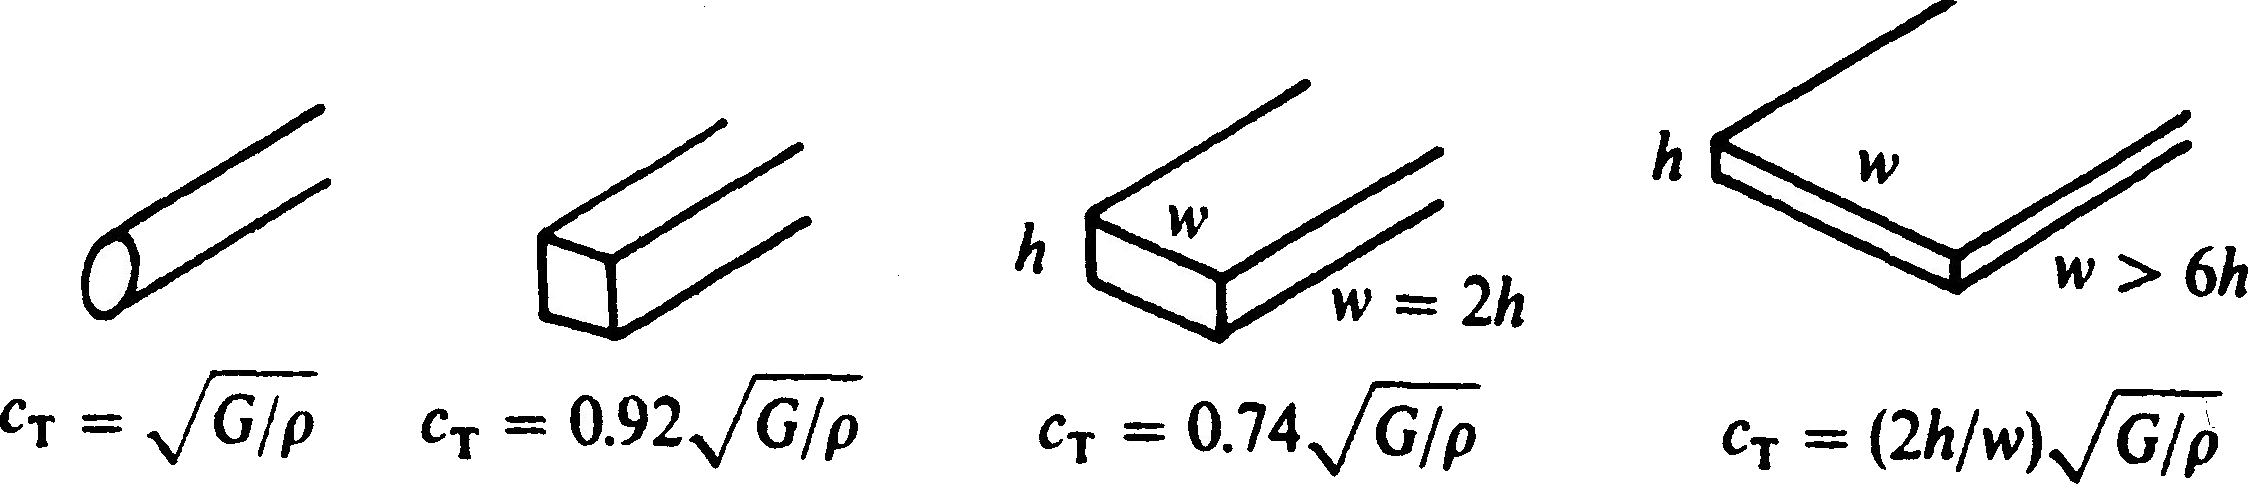
\includegraphics[width=0.9\linewidth]{00_Images/02_chapter/15.png}
    \caption{Torsional wave speed for different bar cross sections}
    \label{fig:torsion_speed_sections}
\end{figure}

\subsection{Standing Waves and Torsional Mode Frequencies}

For a bar of length \( L \), torsional modes follow directly from the nondispersive relation \( \omega = c_t k \). For free-free (or fixed-fixed) ends, the allowed wavenumbers are
\[
k_n = \frac{n\pi}{L},\qquad n = 1,2,3,\dots
\]
leading to the torsional modal frequencies
\[
f_n = \frac{\omega_n}{2\pi} = \frac{n c_t}{2L}
\]
If one end is clamped and the other is free, the quarter-wave condition applies and only odd indices occur,
\[
f_m = \frac{m c_t}{4L},\qquad m = 1,3,5,\dots
\]
in direct analogy with longitudinal modes. 

\paragraph{Torsion in bowed strings} Bowing a violin string excites torsional waves as well as transverse waves. A key point is that \( c_t \) is typically larger than the transverse wave speed \( c \), with reported ratios \( c_t/c \) ranging roughly from \( 2 \) up to \( 7.6 \) depending on string type and construction. The damping of torsional waves (reported around 1\% to 7\%) is dominated by internal damping rather than reflection losses at the bridge and nut and torsional motion affects the effective compliance of the string and the bow-string interaction.

\section{Nonlinear Effects in Strings}

The linear string model assumes that the vibration amplitude is proportional to the excitation amplitude. Whenever this proportionality fails, the behavior is nonlinear. In strings, two broad mechanisms can produce nonlinearity: material effects (elastic moduli depending on strain) and geometric effects. Here we focus on the second mechanism, which becomes relevant when transverse displacements are large.

\subsection{Geometric Nonlinearity: Length Change and Tension Modulation}

Consider the vibration dominated by a single mode \( n \), written (for simplicity) as
\[
y_n(x,t) = a_n\sin\left(\frac{n\pi x}{L}\right)\cos(\omega_n t),
\qquad
\omega_n = \frac{n\pi}{L}\sqrt{\frac{T}{\rho S}}
\]
where \( T \) is the (nominal) tension, \( S \) the cross-sectional area and \( \rho S \) the mass per unit length. Because the string is not perfectly inextensible, transverse motion produces a (second-order) increase of its arc length. The instantaneous length is
\[
L(t) = \int_{0}^{L}\left[1 + \left(\frac{\partial y}{\partial x}\right)^2\right]^{1/2}dx
\]
hence the length variation is
\[
\delta L(t) = L(t)-L
\simeq
\frac{n^{2}\pi^{2}a_n^{2}}{8L}\left(1-\cos 2\omega_n t\right)
\]
This expression contains a steady term and an oscillating term at frequency \( 2\omega_n \). The corresponding tension variation follows from the axial stiffness of the string:
\[
\delta T(t) = \frac{ES}{L}\delta L(t)
 = 
\overline{\delta T} + \Delta T_n\cos(2\omega_n t)
\]
where \( E \) is Young's modulus, \( \overline{\delta T} \) is the steady increase in tension and \( \Delta T_n \) is the amplitude of the oscillating component.

\subsection{Consequences}

\paragraph{Inharmonicity from time-varying tension} Since (in the linear model) modal frequencies scale as \( \omega_n\propto \sqrt{T} \), a small tension modulation produces
\[
\omega_n(t)
 = 
\omega_n\sqrt{1 + \frac{\delta T(t)}{T}}
\simeq
\omega_n\left[1 + \frac{1}{2}\frac{\overline{\delta T}}{T}
 + \frac{1}{2}\frac{\Delta T_n}{T}\cos(2\omega_n t)\right]
\]
The steady term shifts all frequencies upward, while the oscillating term produces a time-varying detuning. Because the magnitude of \( \Delta T_n \) depends on the mode and on the vibration amplitude, different harmonics are affected differently: harmonicity is progressively destroyed until the vibration decays to a sufficiently small level.

\paragraph{Possible countermeasures} Geometric nonlinearity is reduced by using longer strings or with smaller \( E \) or tuned with higher tension \( T \).

\paragraph{Appearance of new modal components} The tension modulation at \( 2\omega_n \) acts as a parametric perturbation. In an ideally clamped string, the oscillating term does not primarily generate components at \( 2\omega_n \), but rather leads to contributions around \( 3\omega_n \). When the termination (bridge) is not perfectly rigid, vibrations near \( 3\omega_n \) can couple into spatial modes and generate the mode \( 2n \). In practice, this effect may be masked when other sources already create spurious oscillations.

\paragraph{Precession of the polarization} Real string motion is generally not confined to a single transverse plane: an oscillation polarized in the \( (x,y) \) plane may coexist with (and excite) an oscillation in the orthogonal \( (x,z) \) plane. The geometric nonlinearity generates components at \( 2\omega_n \) that can set the bridge into motion, providing a forcing path between the two polarizations. As a result, energy is transferred between the two planes and the vibration ellipse precesses. A characteristic rate for this exchange is commonly written as
\[
\Omega = A\frac{ES}{T}\frac{ab}{L^{2}}\omega
\]
where \( A \) is close to unity, \( a \) and \( b \) are the minor and major axes of the polarization ellipse and \( \omega \) is the oscillation frequency. Typical precession time scales are of the order of 1 s and the rate decreases as the vibration amplitude decays.

    %! TEX root = main.tex

\chapter{2D Continuous Systems}

Many sound-radiating structures in musical instruments are not one-dimensional: drumheads, membranes, thin plates and shells are spatially extended in two directions. Their vibration is described by partial differential equations in two spatial variables and the observed motion results from wave propagation on a surface, reflections at boundaries and the formation of 2D standing-wave patterns (modes). This chapter introduces the fundamental 2D models (membranes and plates), derive their wave equations and obtain the modal shapes and eigenfrequencies for simple geometries.

\section{Wave Equation for a Rectangular Membrane}

Consider a rectangular membrane of dimensions \( L_x \) and \( L_y \), under uniform tension \( T \) (\si{\newton\per\metre}) and with mass density per unit area \( \sigma \) (\si{\kilo\gram\per\metre\squared}). Let \( z(x,y,t) \) denote the transverse displacement.

\subsection{Derivation of the Membrane Wave Equation}

\begin{figure}[!htb]
    \centering
    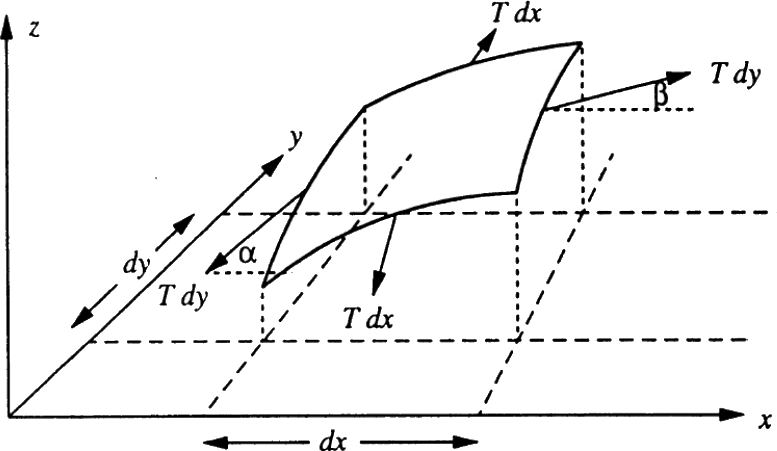
\includegraphics[width=0.75\linewidth]{00_Images/03_chapter/01.png}
    \caption{Forces on an infinitesimal membrane element under uniform tension}
    \label{fig:membrane_element}
\end{figure}

Take an infinitesimal element of membrane with sides \( dx \) and \( dy \). The tension acting on the edge of length \( dx \) is \( Tdx \) (and similarly on the edge \( dy \)). For small slopes, the vertical components of these tensions provide the restoring force. Summing the net vertical force contributions in the \( x \) and \( y \) directions and applying Newton's second law to the element of mass \( \sigma dxdy \) yields the membrane equation of motion:
\[
\frac{\partial^{2}z}{\partial t^{2}}
 = 
\frac{T}{\sigma}
\left(
\frac{\partial^{2}z}{\partial x^{2}}
+
\frac{\partial^{2}z}{\partial y^{2}}
\right)
 = 
c^{2}\nabla^{2}z,
\qquad
c = \sqrt{\frac{T}{\sigma}}
\]
Here \( c \) is the wave speed on the membrane and \( \nabla^{2} \) is the 2D Laplacian in Cartesian coordinates.

\subsection{Separation of Variables and Harmonic Solutions}

For a rectangular domain it is natural to work in Cartesian coordinates and seek separable solutions of the form
\[
z(x,y,t) = X(x)Y(y)\Phi(t)
\]
Substitution gives
\[
\frac{1}{\Phi}\frac{d^{2}\Phi}{dt^{2}}
 = 
c^{2}\left(
\frac{1}{X}\frac{d^{2}X}{dx^{2}}
+
\frac{1}{Y}\frac{d^{2}Y}{dy^{2}}
\right)
\]
Since the left-hand side depends only on \( t \) and the right-hand side depends only on \( x,y \), both must be equal to the same constant. Choosing the constant as \( -\omega^{2} \) yields
\[
\frac{d^{2}\Phi}{dt^{2}}+\omega^{2}\Phi = 0
\quad\Rightarrow\quad
\Phi(t) = E\sin\omega t+F\cos\omega t
\]
and, for the spatial part,
\[
\frac{1}{X}\frac{d^{2}X}{dx^{2}}+\frac{\omega^{2}}{c^{2}}
 = 
-\frac{1}{Y}\frac{d^{2}Y}{dy^{2}}
\]
For this to hold at every point, it sets
\[
\frac{1}{X}\frac{d^{2}X}{dx^{2}} = -h^{2},
\qquad
\frac{1}{Y}\frac{d^{2}Y}{dy^{2}} = -r^{2},
\qquad
h^{2}+r^{2} = \frac{\omega^{2}}{c^{2}}
\]
so that
\[
X(x) = A\sin(hx)+B\cos(hx),
\qquad
Y(y) = C\sin(ry)+D\cos(ry)
\]
The parameters \( h \) and \( r \) determine the spatial periodicity along \( x \) and \( y \), respectively. 

\subsection{Fixed-Edge Boundary Conditions and Natural Frequencies}

For a membrane clamped along its boundary, the displacement vanishes at the edges:
\[
z = 0 \quad \text{at} \quad x = 0,\ x = L_x,\ y = 0,\ y = L_y
\]
The conditions at \( x = 0 \) and \( y = 0 \) imply \( B = 0 \) and \( D = 0 \). Imposing \( z(L_x,y,t) = 0 \) requires
\[
\sin(hL_x) = 0 \quad\Rightarrow\quad h = \frac{m\pi}{L_x},
\qquad m = 1,2,3,\dots
\]
and imposing \( z(x,L_y,t) = 0 \) requires
\[
\sin(rL_y) = 0 \quad\Rightarrow\quad r = \frac{n\pi}{L_y},
\qquad n = 1,2,3,\dots
\]
Therefore the \( (m,n) \) -th mode shape is
\[
z_{mn}(x,y,t) = A\sin\left(\frac{m\pi}{L_x}x\right)\sin\left(\frac{n\pi}{L_y}y\right)
\left(E\sin\omega_{mn}t+F\cos\omega_{mn}t\right)
\]
with
\[
\omega_{mn} = c\sqrt{h^{2}+r^{2}}
 = 
c\pi\sqrt{\left(\frac{m}{L_x}\right)^{2}+\left(\frac{n}{L_y}\right)^{2}}
\]
and the natural frequencies
\[
f_{mn} = \frac{\omega_{mn}}{2\pi}
 = 
\frac{1}{2}\sqrt{\frac{T}{\sigma}}
\sqrt{\left(\frac{m}{L_x}\right)^{2}+\left(\frac{n}{L_y}\right)^{2}}
\]
As usual, \( m = 0 \) or \( n = 0 \) (and in particular \( m = n = 0 \)) corresponds to the trivial solution \( z = 0 \).

\paragraph{Square membranes and modal degeneracy} If \( L_x = L_y \), then \( f_{mn} = f_{nm} \): distinct mode shapes can share the same eigenfrequency. In that case, any linear combination
\[
z(x,y,t) = \left(az_{mn}+bz_{nm}\right)\cos\omega t,
\qquad a^{2}+b^{2} = 1
\]
is also a valid vibration pattern at the same frequency and the observed nodal lines depend on the combination coefficients.

\begin{figure}[!htb]
    \centering
    \subfloat[Degenerate modes in a square membrane]{%
        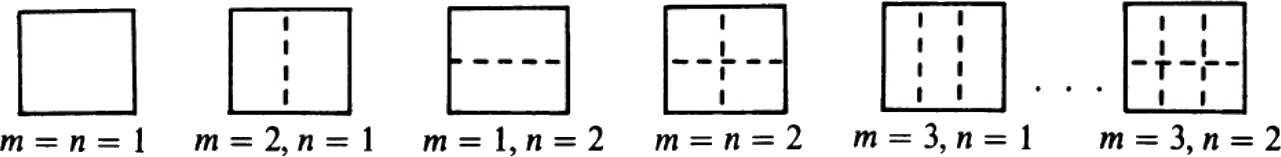
\includegraphics[width=0.9\linewidth]{00_Images/03_chapter/02.png}%
    }\\
    \subfloat[Linear combinations and resulting nodal patterns]{%
        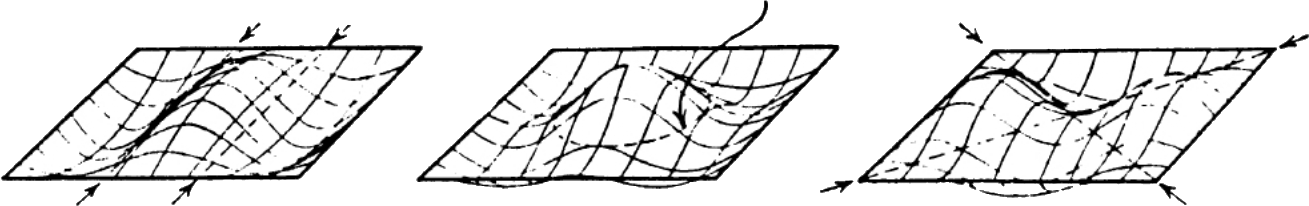
\includegraphics[width=0.9\linewidth]{00_Images/03_chapter/03.png}%
    }
    \caption{Modal degeneracy in a square membrane}
    \label{fig:square_membrane_degeneracy}
\end{figure}

\section{Circular Membranes}

For a circular membrane the boundary condition imposes that the transverse displacement vanishes on the circular edge. It places the origin at the center of the membrane, uses polar coordinates \( (r,\varphi) \) and denotes by \( a \) the membrane radius.

\subsection{Wave Equation in Polar Coordinates}

For a membrane under uniform tension \( T \) (\si{\newton\per\metre}) and surface mass density \( \sigma \) (\si{\kilo\gram\per\metre\squared}), the equation of motion becomes
\[
\frac{\partial^{2}z}{\partial t^{2}}
 = 
c^{2}\left(
\frac{\partial^{2}z}{\partial r^{2}}
+\frac{1}{r}\frac{\partial z}{\partial r}
+\frac{1}{r^{2}}\frac{\partial^{2}z}{\partial \varphi^{2}}
\right),
\qquad
c = \sqrt{\frac{T}{\sigma}}
\]
The clamped-edge condition is
\[
z(a,\varphi,t) = 0 \quad \text{for all } \varphi,t
\]

\subsection{Separation of Variables and Bessel Functions}

\begin{figure}[!htb]
    \centering
    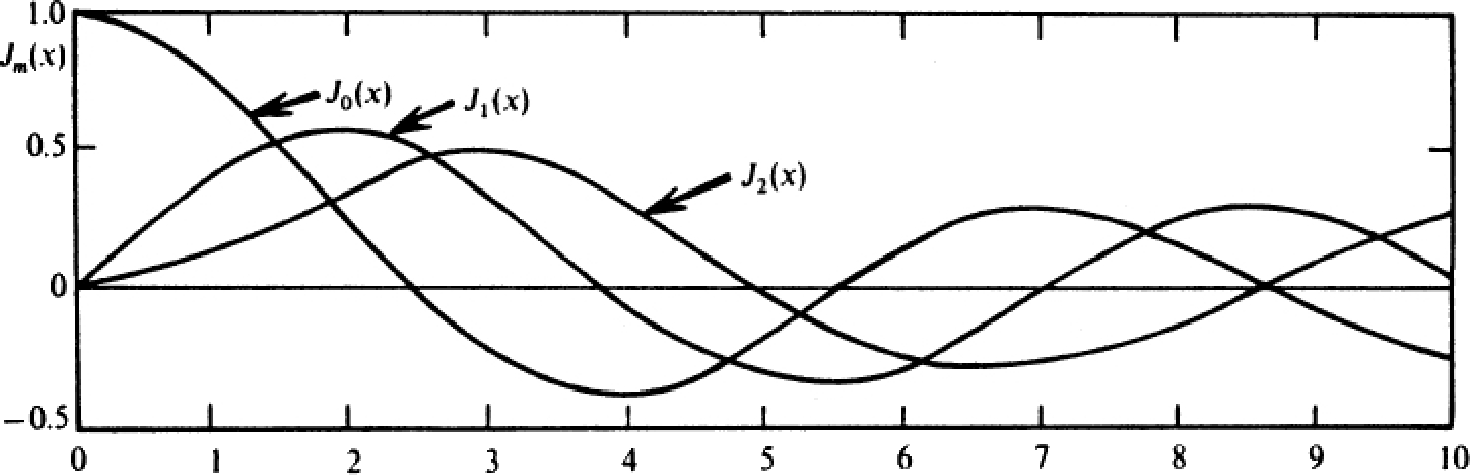
\includegraphics[width=0.8\linewidth]{00_Images/03_chapter/04.png}
    \caption{Bessel functions (first kind) and their zeros}
    \label{fig:bessel_zeros}
\end{figure}

Assume a harmonic separable solution
\[
z_e(r,\varphi,t) = R(r)\Phi(\varphi)e^{j\omega t}
\]
Substitution yields two ordinary differential equations. The angular part is
\[
\frac{d^{2}\Phi}{d\varphi^{2}}+m^{2}\Phi = 0
\qquad\Rightarrow\qquad
\Phi(\varphi) = A e^{\pm jm\varphi}
\]
where \( m\in\mathbb{Z} \) is the azimuthal order. The radial part becomes
\[
\frac{d^{2}R}{dr^{2}}+\frac{1}{r}\frac{dR}{dr}
+\left(\frac{\omega^{2}}{c^{2}}-\frac{m^{2}}{r^{2}}\right)R = 0
\]
This is Bessel's equation. The physically acceptable solution at \( r = 0 \) is the Bessel function of the first kind,
\[
R(r) = J_m(kr),
\qquad
k = \frac{\omega}{c}
\]

\subsection{Boundary Condition, Eigenvalues and Natural Frequencies}

The clamped boundary condition \( z(a,\varphi,t) = 0 \) implies
\[
J_m(ka) = 0
\]
Let \( Z_{mn} \) denote the \( n \) -th positive zero of \( J_m(\cdot) \). Then the admissible wavenumbers are
\[
k_{mn} = \frac{Z_{mn}}{a}
\]
and the natural (angular) frequencies are
\[
\omega_{mn} = ck_{mn} = c\frac{Z_{mn}}{a},
\qquad
f_{mn} = \frac{\omega_{mn}}{2\pi}
 = 
\frac{Z_{mn}}{2\pi a}\sqrt{\frac{T}{\sigma}}
\]
As an example, for the fundamental axisymmetric mode \( (m,n) = (0,1) \) one has \( Z_{01} \simeq 2.405 \), hence
\[
f_{01} = 
\frac{2.405}{2\pi a}\sqrt{\frac{T}{\sigma}}
\]

\subsection{Mode Shapes and Nodal Patterns}

\begin{figure}[!htb]
    \centering
    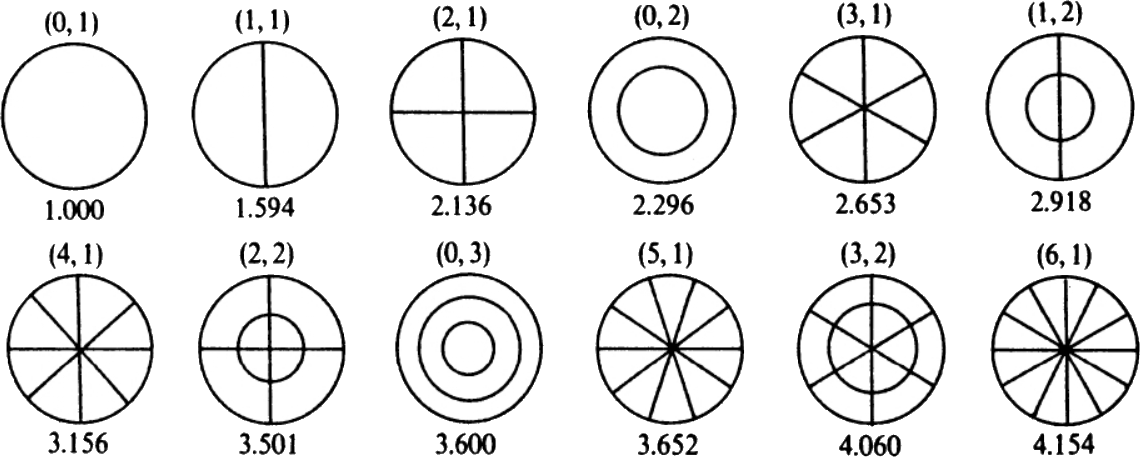
\includegraphics[width=0.9\linewidth]{00_Images/03_chapter/05.png}
    \caption{Normal modes of a circular membrane (nodal diameters and circles)}
    \label{fig:circular_membrane_modes}
\end{figure}

The (complex) modal shape can be written as
\[
z_{emn}(r,\varphi) = \Phi(\varphi)R(r) = A e^{\pm jm\varphi}J_m(k_{mn}r)
\]
and the overall (complex) displacement is a modal superposition
\[
z_e(r,\varphi,t) = \sum_{m}\sum_{n} c_{mn}z_{emn}(r,\varphi)e^{j\omega_{mn}t},
\qquad
z(r,\varphi,t) = \Re\{z_e(r,\varphi,t)\}
\]
where the coefficients \( c_{mn} \) depend on the excitation. Geometrically, the \( (m,n) \) -th mode has:

\begin{itemize}
    \item \( m \) nodal diameters (lines through the center);
    \item \( n \) nodal circles (concentric rings), counting the boundary as the outer zero.
\end{itemize}

In particular, \( (0,1) \) entails an in-phase displacement of the whole membrane, while \( (1,1) \) is an antisymmetric motion of the two halves. 

\paragraph{Remark on air loading} When the membrane is in contact with air, modal frequencies are generally lowered. In a kettledrum, where the air is confined, axisymmetric modes such as \( (0,1) \) are raised, while the remaining modes are lowered. 

\section{Elastic Materials and Mechanical Parameters}

Now, it is useful to summarize the constitutive parameters that control wave propagation in solids. In continuum mechanics, external loads generate a stress field, which in turn produces a strain field according to material-dependent constitutive equations. For linear elastic media, these relations are linear and can be expressed compactly in tensor or matrix form. 

\subsection{Stress, Strain and Generalized Hooke's Law}

Consider a deformable solid (e.g. a small cube). The stress tensor \( \sigma_{ij} \) represents the force per unit area acting on the face orthogonal to axis \( i \), directed along axis \( j \). Similarly, the strain tensor \( \varepsilon_{kl} \) quantifies the deformation. In matrix form,
\[
\symbf{\sigma} = 
\begin{bmatrix}
\sigma_{xx} & \sigma_{xy} & \sigma_{xz}\\
\sigma_{yx} & \sigma_{yy} & \sigma_{yz}\\
\sigma_{zx} & \sigma_{zy} & \sigma_{zz}
\end{bmatrix},
\qquad
\symbf{\varepsilon} = 
\begin{bmatrix}
\varepsilon_{xx} & \varepsilon_{xy} & \varepsilon_{xz}\\
\varepsilon_{yx} & \varepsilon_{yy} & \varepsilon_{yz}\\
\varepsilon_{zx} & \varepsilon_{zy} & \varepsilon_{zz}
\end{bmatrix}
\]
In general, a single stress component \( \sigma_{ij} \) can generate several strain components \( \varepsilon_{kl} \). The most general linear elastic constitutive relation is the generalized Hooke's law
\[
\sigma_{ij} = A_{ijkl}\varepsilon_{kl}
\]
where \( A_{ijkl} \) is the elasticity tensor (fourth-rank). It has \( 3^4 = 81 \) components, reduced by symmetry considerations (stress and strain tensors are symmetric) and by energy arguments down to 21 independent constants in the fully anisotropic case. 

\subsection{Uniaxial Traction: Young's Modulus and Yield Strength}

\begin{figure}[!htb]
    \centering
    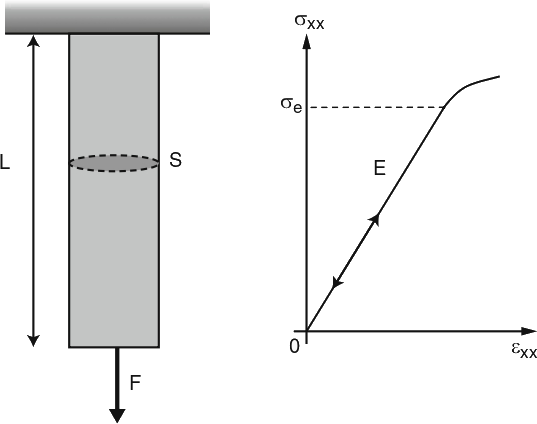
\includegraphics[width=0.6\linewidth]{00_Images/03_chapter/06.png}
    \caption{Uniaxial traction and a typical stress-strain curve}
    \label{fig:uniaxial_traction}
\end{figure}

A basic experiment to characterize stiffness is uniaxial traction of a slender specimen (length \( L_0 \) much larger than its lateral size). If a tensile force \( F \) is applied along \( x \), the axial stress and strain are approximated by
\[
\sigma_{xx} \simeq \frac{F}{S},
\qquad
\varepsilon_{xx} \simeq \frac{L-L_0}{L_0}
\]
In the linear reversible regime (below the yield strength \( \sigma_e \)), stress and strain are proportional,
\[
\sigma_{xx} = E\varepsilon_{xx}
\]
where \( E \) is Young's modulus. Beyond \( \sigma_e \), the stress-strain curve is no longer linear and at higher stress the specimen ultimately fails (ultimate tensile strength). Typical values for \( E \), \( \sigma_e \) and ultimate strength vary greatly across materials (metals, polymers, glass, etc.). 

\subsection{Poisson's Ratio and the Poisson Effect}

\begin{figure}[!htb]
    \centering
    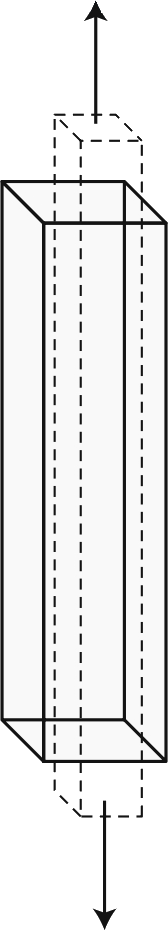
\includegraphics[height=0.3\textheight]{00_Images/03_chapter/07.png}
    \caption{Poisson effect under uniaxial loading}
    \label{fig:poisson_effect}
\end{figure}

Under uniaxial traction along \( x \), real solids  contract laterally. In the simplest isotropic linear model, 
\[
\varepsilon_{yy} = -\nu\frac{\sigma_{xx}}{E},
\qquad
\varepsilon_{zz} = -\nu\frac{\sigma_{xx}}{E}
\]
where \( \nu \) is Poisson's ratio. Thus \( \nu \) measures the lateral compression under axial extension (Poisson effect). For most standard materials \( 0<\nu<1/2 \), but special auxetic materials exhibit an effective \( \nu<0 \), i.e. they expand laterally when stretched due to their microstructure. 

\subsection{Shear Modulus}

\begin{figure}[!htb]
    \centering
    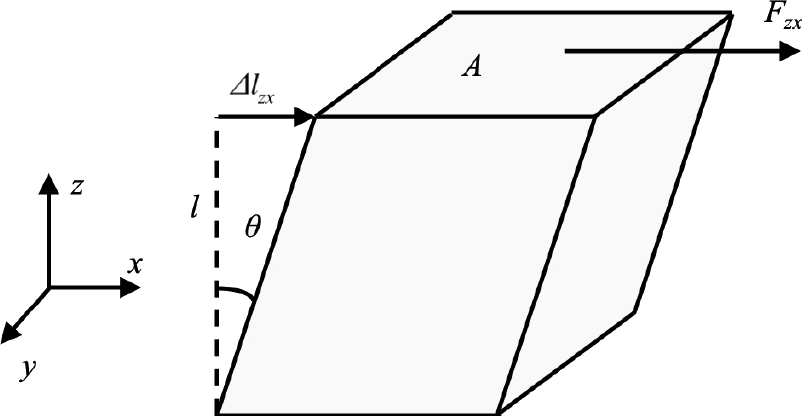
\includegraphics[width=0.65\linewidth]{00_Images/03_chapter/08.png}
    \caption{Shear deformation defining the shear modulus \(G\)}
    \label{fig:shear_modulus}
\end{figure}

A second independent elastic parameter is the shear (torsional) modulus \( G \), defined as the ratio between shear stress and shear strain. For the shear component \( (z,x) \), 
\[
G = \frac{\sigma_{zx}}{\gamma_{zx}}
 = 
\frac{F_{zx}/A}{\Delta l_{zx}/l}
 = 
\frac{F_{zx}l}{A\Delta l_{zx}}
\]
where \( A \) is the sheared area, \( l \) the specimen height and \( \gamma_{zx}\simeq\tan\theta \simeq \theta \) is the (small) shear strain. Values of \( G \) also span orders of magnitude across materials. 

\subsection{Voigt Notation and Matrix Constitutive Equations}

Because \( \sigma \) and \( \varepsilon \) are symmetric, it is convenient to collect their independent components into 6-vectors (Voigt notation):
\[
\vv{\sigma}_V = 
\begin{bmatrix}
\sigma_{xx}&\sigma_{yy}&\sigma_{zz}&\sigma_{zx}&\sigma_{yz}&\sigma_{xy}
\end{bmatrix}^{T},
\qquad
\vv{\varepsilon}_V = 
\begin{bmatrix}
\varepsilon_{xx}&\varepsilon_{yy}&\varepsilon_{zz}&\varepsilon_{zx}&\varepsilon_{yz}&\varepsilon_{xy}
\end{bmatrix}^{T}
\]
Then the constitutive law becomes a \( 6 \times 6 \) matrix relation,
\[
\vv{\sigma}_V = \symbf{A}_V\vv{\varepsilon}_V
\]
This form is particularly useful in plate and shell models, where bending stiffness and wave propagation constants can be expressed directly in terms of elastic matrix entries.

\subsection{Isotropic Materials: the Lamé Parameters}

In an isotropic material all directions are equivalent and linear elasticity is fully characterized by two constants (Lamé parameters \( \lambda \) and \( \mu \)). In Voigt notation the stiffness matrix takes the standard form
\[
\begin{bmatrix}
\sigma_{xx}\\\sigma_{yy}\\\sigma_{zz}\\\sigma_{zx}\\\sigma_{yz}\\\sigma_{xy}
\end{bmatrix}
 = 
\begin{bmatrix}
\lambda+2\mu & \lambda      & \lambda      & 0   & 0   & 0\\
\lambda      & \lambda+2\mu & \lambda      & 0   & 0   & 0\\
\lambda      & \lambda      & \lambda+2\mu & 0   & 0   & 0\\
0            & 0            & 0            & 2\mu& 0   & 0\\
0            & 0            & 0            & 0   & 2\mu& 0\\
0            & 0            & 0            & 0   & 0   & 2\mu
\end{bmatrix}
\begin{bmatrix}
\varepsilon_{xx}\\\varepsilon_{yy}\\\varepsilon_{zz}\\\varepsilon_{zx}\\\varepsilon_{yz}\\\varepsilon_{xy}
\end{bmatrix}
\]
The Lamé parameters can be expressed in terms of Young's modulus \( E \) and Poisson's ratio \( \nu \) as:
\[
\lambda = \frac{E\nu}{(1+\nu)(1-2\nu)},
\qquad
\mu = \frac{E}{2(1+\nu)}
\]
In particular, \( \mu \) coincides with the shear modulus \( G \) for isotropic media.

\subsection{Orthotropic Materials: Wood and Directional Elasticity}

\begin{figure}[!htb]
    \centering
    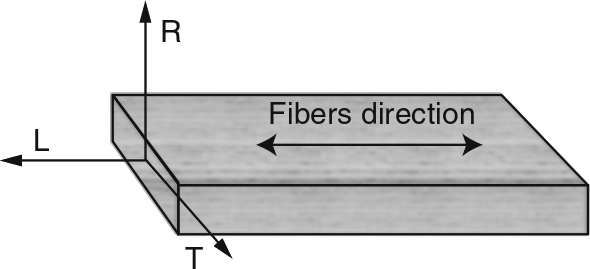
\includegraphics[width=0.78\linewidth]{00_Images/03_chapter/09.png}
    \caption{Orthotropic axes in wood: longitudinal (L), radial (R), tangential (T)}
    \label{fig:wood_axes}
\end{figure}

Many musical materials are anisotropic. Wood is often modeled as orthotropic, meaning that its elastic properties differ along three orthogonal material directions: longitudinal \( L \) (along the fibers), radial \( R \) (along growth-ring radii) and tangential \( T \) (tangent to growth rings). In this case, it is convenient to write the compliance form (strain as a function of stress). For axes aligned with \( x = L \), \( y = R \), \( z = T \), the Voigt relation becomes:
\[
\begin{bmatrix}
\varepsilon_{xx}\\\varepsilon_{yy}\\\varepsilon_{zz}\\\varepsilon_{zx}\\\varepsilon_{yz}\\\varepsilon_{xy}
\end{bmatrix}
 = 
\begin{bmatrix}
\frac{1}{E_L} & -\frac{\nu_{RL}}{E_R} & -\frac{\nu_{TL}}{E_T} & 0 & 0 & 0\\
-\frac{\nu_{LR}}{E_L} & \frac{1}{E_R} & -\frac{\nu_{TR}}{E_T} & 0 & 0 & 0\\
-\frac{\nu_{LT}}{E_L} & -\frac{\nu_{RT}}{E_R} & \frac{1}{E_T} & 0 & 0 & 0\\
0 & 0 & 0 & \frac{1}{2G_{LT}} & 0 & 0\\
0 & 0 & 0 & 0 & \frac{1}{2G_{TR}} & 0\\
0 & 0 & 0 & 0 & 0 & \frac{1}{2G_{RL}}
\end{bmatrix}
\begin{bmatrix}
\sigma_{xx} \\
\sigma_{yy} \\
\sigma_{zz} \\
\sigma_{zx} \\
\sigma_{yz} \\
\sigma_{xy}
\end{bmatrix}
\]
The orthotropic elastic behavior is described by nine independent coefficients: 

\begin{itemize}
    \item three Young's moduli \( E_L, E_R, E_T \),
    \item three Poisson ratios (e.g. \( \nu_{LR}, \nu_{RT}, \nu_{TL} \)),
    \item three shear moduli \( G_{LT}, G_{TR}, G_{RL} \).
\end{itemize}

The remaining Poisson ratios are determined by symmetry constraints (\( \nu_{LR}/E_L = \nu_{RL}/E_R \) and similarly for the other pairs). For spruce soundboards, a typical feature is the strong anisotropy \( E_L/E_T \) (often of order \( 10 \) to \( 20 \)), which is one of the key reasons why the orientation of the grain matters in instrument making. 

\section{Waves in Thin Plates}

The previous section introduced the elastic constants (\( E,\nu,G \)) and the density \( \rho \), which fully determine (together with thickness \( h \)) the propagation of mechanical waves in thin plates. Unlike membranes, plates possess bending stiffness, so waves can propagate even in the absence of any applied in-plane tension. In thin plates three main families of waves are commonly distinguished: quasi-longitudinal waves, torsional (in-plane shear) waves and bending (flexural) waves.

\begin{figure}[!htb]
    \centering
    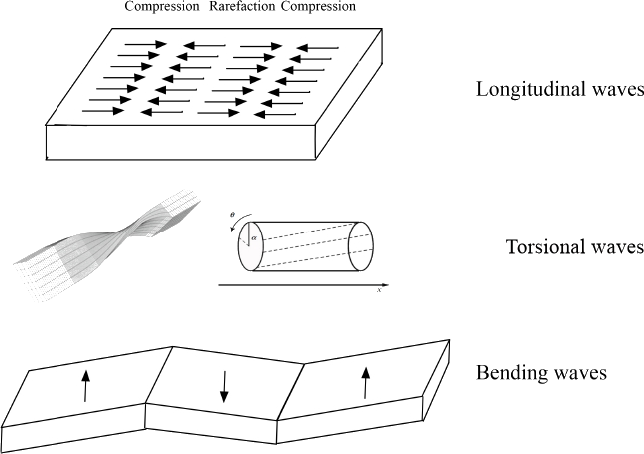
\includegraphics[width=0.6\linewidth]{00_Images/03_chapter/10.png}
    \caption{Wave types in thin plates: quasi-longitudinal, torsional, and bending}
    \label{fig:plate_wave_types}
\end{figure}

\subsection{Quasi-Longitudinal Waves}

\begin{figure}[!htb]
    \centering
    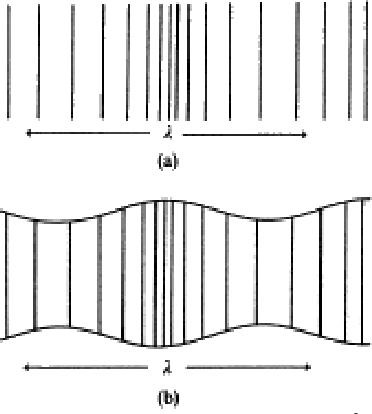
\includegraphics[width=0.5\linewidth]{00_Images/03_chapter/11.png}
    \caption{Quasi-longitudinal deformation in a thin plate}
    \label{fig:quasi_longitudinal_plate}
\end{figure}

Longitudinal waves in plates do not propagate at the same speed as longitudinal waves in bars made of the same material. When a longitudinal wave propagates in a thin plate, it induces a slight expansion/compression in the direction orthogonal to the wavefront through the Poisson effect; this modifies the local stiffness and changes the wave speed. For this reason they are referred to as quasi-longitudinal waves. Purely longitudinal waves occur only in solids whose dimensions are all much larger than the wavelength. The propagation velocity of quasi-longitudinal waves in a plate is
\[
c_L = \sqrt{\frac{E}{\rho(1-\nu^{2})}}
\]
where \( E \) is Young's modulus, \( \rho \) is the material density and \( \nu \) is Poisson's ratio. For comparison, a purely longitudinal wave (3D bulk) would propagate at
\[
c_L' = \sqrt{\frac{E(1-\nu)}{\rho(1+\nu)(1-2\nu)}}
\]
while the classical 1D bar result is
\[
c_{L,\mathrm{bar}} = \sqrt{\frac{E}{\rho}}
\]
These expressions make explicit that the plate velocity differs from the bar velocity because \( \nu\neq 0 \) couples axial and lateral strains. 

\subsection{Torsional (In-Plane Shear) Waves}

Torsional waves in a thin plate propagate at the same speed as torsional waves in a rod, namely
\[
c_T = \sqrt{\frac{G}{\rho}}
\]
where \( G \) is the shear modulus. Since typically \( G<E \), torsional waves propagate slower than longitudinal (or quasi-longitudinal) waves. Torsional and quasi-longitudinal waves involve particle motion that is largely tangential to the plate surface; consequently, they are comparatively inefficient for airborne sound radiation. In musical applications they may still be relevant because their modal frequencies are generally not in harmonic correspondence with the main flexural components and can therefore produce perceptually annoying or unexpected features if strongly excited.

\subsection{Bending (Flexural) Waves}

The most important waves for sound radiation from plates are bending waves, because they involve out-of-plane motion. Let \( z(x,y,t) \) be the transverse displacement of a thin plate of thickness \( h \). In the Kirchhoff-Love thin-plate approximation, bending waves satisfy
\[
\frac{\partial^{2}z}{\partial t^{2}}
+
\frac{E h^{2}}{12\rho(1-\nu^{2})}\nabla^{4}z
 = 0
\]
where \( \nabla^{4} = \nabla^{2}\nabla^{2} \) is the biharmonic operator in the plate plane. Assuming a harmonic time dependence,
\[
z(x,y,t) = Z(x,y)e^{j\omega t}
\]
and substituting yields
\[
\nabla^{4}Z-\frac{12\rho(1-\nu^{2})\omega^{2}}{Eh^{2}}Z = 0
\quad\Longleftrightarrow\quad
\nabla^{4}Z-k^{4}Z = 0
\]
where the (frequency-dependent) bending wavenumber is defined by
\[
k^{4} = \frac{12\rho(1-\nu^{2})\omega^{2}}{Eh^{2}}
\qquad\Rightarrow\qquad
k^{2} = \frac{\sqrt{12}\omega}{h}\sqrt{\frac{\rho(1-\nu^{2})}{E}}
 = \frac{\sqrt{12}\omega}{hc_L}
\]
In general, \( Z(x,y) \) is not separable in \( x \) and \( y \); the admissible values of \( k \) (hence the modal frequencies) depend on the plate geometry and boundary conditions.

\paragraph{Dispersion} Flexural waves are dispersive. The dispersion relation can be read from the scaling above as
\[
\omega  \propto k^{2}
\]
hence the phase velocity increases with frequency. Using the definitions, one obtains
\[
v(\omega) = \frac{\omega}{k}
 = \sqrt{\frac{\omega h c_L}{\sqrt{12}}}
 \simeq \sqrt{1.8fhc_L}
\]
and equivalently
\[
f = \frac{\omega}{2\pi} = 0.0459hc_Lk^{2}
\]
Therefore, higher-frequency bending components travel faster and sharp features of a waveform tend to spread as they propagate across the plate. 

\section{Bending Waves in Circular Plates}

Consider a thin circular plate of radius \( a \) and thickness \( h \), made of a homogeneous isotropic material with density \( \rho \), Young's modulus \( E \) and Poisson's ratio \( \nu \). Let \( z(r,\varphi,t) \) denote the transverse displacement in polar coordinates. For bending (flexural) motion, the harmonic response \( z(r,\varphi,t) = \Re\{Z(r,\varphi)e^{j\omega t}\} \) satisfies the plate equation
\[
\nabla^{4}Z-k^{4}Z = 0,
\qquad
k^{2} = \frac{\sqrt{12}\omega}{hc_L},
\qquad
c_L = \sqrt{\frac{E}{\rho(1-\nu^{2})}}
\]
so that the modal frequencies can be written as
\[
f = \frac{\omega}{2\pi}
 = \frac{hc_L}{2\pi\sqrt{12}}k^{2}
 \simeq 0.0459hc_Lk^{2}
\]

\subsection{General Harmonic Solution in Polar Coordinates}

A standard factorization of the biharmonic operator leads to two Helmholtz-type equations,
\[
(\nabla^{2}+k^{2})Z = 0,
\qquad
(\nabla^{2}-k^{2})Z = 0
\]
whose separable solutions in polar coordinates involve Bessel functions. For azimuthal order \( m\in\mathbb{N} \), one finds
\[
(\nabla^{2}+k^{2})Z = 0
\quad\Rightarrow\quad
Z(r,\varphi) = Ae^{jm\varphi}J_m(kr)
\]
\[
(\nabla^{2}-k^{2})Z = 0
\quad\Rightarrow\quad
Z(r,\varphi) = Be^{jm\varphi}I_m(kr)
\]
where \( J_m(\cdot) \) is the Bessel function of the first kind and \( I_m(\cdot) \) is the modified (hyperbolic) Bessel function. A real-valued representation is conveniently written as
\[
Z(r,\varphi) = \cos(m\varphi+\alpha)\left[AJ_m(kr)+BI_m(kr)\right]
\]
with \( \alpha \) setting the orientation of the nodal diameters.

\subsection{Edge Conditions, Wavenumbers and Modal Frequencies}

The admissible values of \( k \) (hence the eigenfrequencies) are fixed by the boundary conditions at the rim \( r = a \). Three idealizations are commonly used.

\paragraph{Clamped Edge} For a clamped boundary the displacement and slope vanish at the rim,
\[
Z(a,\varphi) = 0,
\qquad
\left.\frac{\partial Z}{\partial r}\right|_{r = a} = 0
\]
These two conditions yield a discrete set of wavenumbers \( k_{mn} \) (no closed-form expression). The first values reported are 
\[
k_{01} = \frac{3.189}{a},\quad
k_{11} = \frac{4.612}{a},\quad
k_{21} = \frac{5.904}{a}
\]
\[
k_{02} = \frac{6.308}{a},\quad
k_{12} = \frac{7.801}{a},\quad
k_{22} = \frac{9.400}{a}
\]
\[
k_{03} = \frac{9.425}{a},\quad
k_{13} = \frac{10.965}{a},\quad
k_{23} = \frac{12.566}{a},
\qquad
k_{mn}\to \frac{(2n+m)\pi}{a}\ \text{as } n\to\infty
\]
Using \( f \simeq 0.0459hc_Lk^2 \), the corresponding modal frequencies can be written compactly in normalized form. Defining
\[
f_{01} = 0.4694\frac{c_L h}{a^{2}}
\]
one obtains (examples)
\[
f_{11} = 2.08f_{01},\quad
f_{21} = 3.41f_{01},\quad
f_{02} = 3.89f_{01},\quad
f_{12} = 5.95f_{01},\quad
f_{03} = 8.72f_{01}
\]
with higher families following the same pattern. 

\paragraph{Free Edge} For a free boundary, bending moment and shear force vanish at the rim (hence boundary conditions involve second and third radial derivatives). The asymptotic behavior for large \( ka \) is
\[
k_{mn} \approx \frac{(2n+m)\pi}{2a}
\]
A notable feature is that the fundamental mode is not \( (0,1) \) but \( (2,0) \). Defining
\[
f_{20} = 0.2413\frac{c_L h}{a^{2}}
\]
the modal frequencies are conveniently listed as multiples of \( f_{20} \), e.g.
\[
f_{01} = 1.73f_{20},\quad f_{11} = 3.91f_{20},\quad
f_{02} = 7.34f_{20},\quad f_{21} = 6.71f_{20}
\]
and so on for higher orders. 

\paragraph{Supported Edge} For a simply supported circular plate, the displacement vanishes at the rim while the bending moment is zero (again yielding a discrete spectrum). The fundamental frequency is reported as
\[
f_{01} = 0.2287\frac{c_L h}{a^{2}}
\]
and higher modes can be expressed as multiples of \( f_{01} \), for instance
\[
f_{11} = 2.80f_{01},\quad
f_{21} = 5.15f_{01},\quad
f_{02} = 5.98f_{01},\quad
f_{12} = 9.75f_{01}
\]

\paragraph{Mode identification} As for circular membranes, the index \( m \) counts the number of nodal diameters, while the radial order \( n \) counts nodal circles.

\section{Bending Waves in Rectangular Plates}

Now, consider a thin rectangular plate of dimensions \( L_x \times L_y \), thickness \( h \), made of an isotropic material with density \( \rho \), Young's modulus \( E \) and Poisson's ratio \( \nu \). As in the previous section, bending (flexural) motion is governed by the biharmonic plate equation and the admissible mode shapes and eigenfrequencies depend strongly on the boundary conditions at the edges. 

\subsection{Supported Edges: Separable Modes and Closed-Form Frequencies}

For a plate simply supported on all four edges, the transverse displacement vanishes at the boundary and the resulting bending modes are separable in Cartesian coordinates. The spatial part of the displacement can be written as
\[
Z(x,y) = A
\sin\left(\frac{(m+1)\pi}{L_x}x\right)
\sin\left(\frac{(n+1)\pi}{L_y}y\right),
\qquad m,n = 0,1,2,\dots
\]
which is formally identical (in shape) to the rectangular membrane case: nodal lines are straight and parallel to the edges and the indices \( m,n \) count the number of half-wavelengths along \( x \) and \( y \). The corresponding modal frequencies are given as
\[
f_{mn}
 = 
0.453c_Lh
\left[
\frac{(m+1)^2}{L_x^2}
+
\frac{(n+1)^2}{L_y^2}\right]
\qquad
c_L = \sqrt{\frac{E}{\rho(1-\nu^2)}}
\]
Hence \( f_{mn} \propto h \) and grows with stiffness through \( c_L \), while increasing plate dimensions lowers the eigenfrequencies. In the square case \( L_x = L_y \), frequency degeneracy occurs whenever \( (m,n) \) and \( (n,m) \) produce the same value of the square-root term.

\subsection{Free Edges: Mode Mixing and the Role of Poisson Coupling}

For a plate with free edges, the exact derivation is substantially more involved and the mode shapes are no longer well represented by a simple product of two independent sine functions.

\paragraph{Aspect ratio limit} If \( L_x/L_y \gg 1 \), the plate behaves increasingly like a bar: flexural modes resemble those of a thin bar and the motion is dominated by bending along the long direction.

\paragraph{Mixed modes when \( L_x \) and \( L_y \) are comparable} When the aspect ratio approaches unity, a wave pattern primarily propagating along \( x \) induces deformation along \( y \) as well, effectively changing the stiffness and distorting the nodal patterns. The nodal-line examples (for \( L_x/L_y = 2 \) and \( L_x/L_y = 3/2 \)) illustrate how the shapes depart from the purely separable patterns of the supported case.

\paragraph{Poisson ratio as coupling parameter} The parameter \( \nu \) quantifies the coupling between orthogonal deformations: bending along one axis generates strains along the other axis via the Poisson effect. This coupling is the reason why, for free plates, families of modes can hybridize as the aspect ratio changes. A particularly important example is the interaction between the two modes often labeled \( (2,0) \) and \( (0,2) \). As the aspect ratio varies from \( L_x/L_y = 4 \) down to \( 1 \), these two shapes combine into two distinct superpositions:
\[
(2,0)-(0,2)\quad \text{(x mode}),
\qquad
(2,0)+(0,2)\quad \text{(ring mode})
\]
For a square plate (\( L_x = L_y \)), the mixing becomes complete: the observed nodal patterns correspond to these combined shapes rather than to two independent, uncoupled modes. When plotting normalized frequencies versus aspect ratio, the ring mode remains almost constant, while the x-mode frequency increases approximately linearly with \( L_x/L_y \). Moreover, the degeneracy that would be expected from symmetry is resolved: the two mixed modes split in frequency because the plate responds differently to the additive and subtractive combinations, an effect induced by Poisson coupling. This behavior is reported in figure \ref{fig:rect_plate_mode_mixing}.

\begin{figure}[!htb]
    \centering
    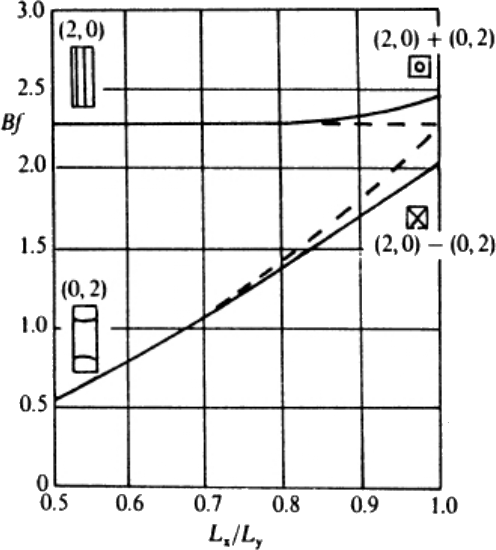
\includegraphics[width=0.5\linewidth]{00_Images/03_chapter/14.png}
    \caption{Frequencies of the vibrational modes as a function of the aspect ratio}
    \label{fig:rect_plate_mode_mixing}
\end{figure}

\section{Bending Waves in Square Plates}

\begin{figure}[!htb]
    \centering
    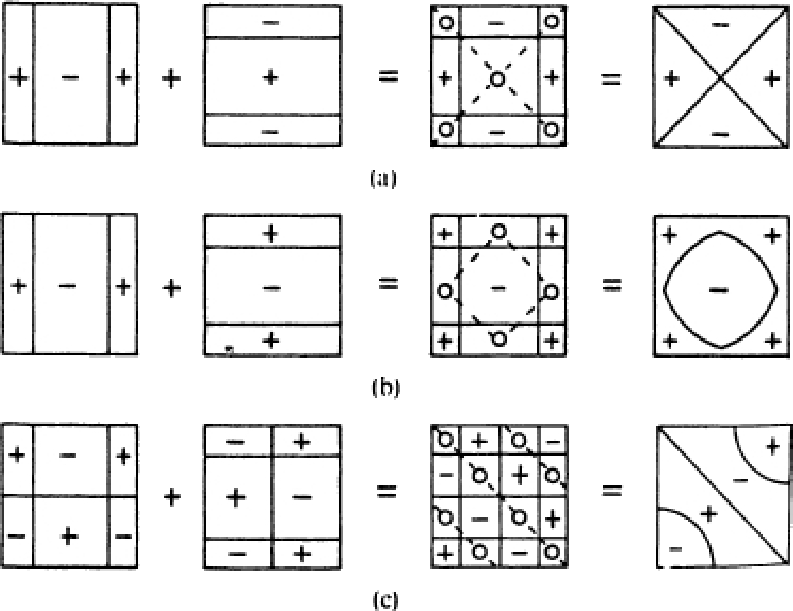
\includegraphics[width=0.7\linewidth]{00_Images/03_chapter/15.png}
    \caption{Graphical construction of the interaction between different modes of a square plate}
    \label{fig:square_plate_modes}
\end{figure}

Square plates (\( L_x = L_y = L \)) are a special case because symmetry forces pairs of rectangular-plate modes \( (m,n) \) and \( (n,m) \) to interact. In membranes this interaction leads to true degeneracy (same frequency). In thin plates, instead, Poisson coupling modifies the stiffness and can split the frequencies of the mixed combinations.

\subsection{Complete Mixing of \texorpdfstring{ \( (2,0) \) }{(2,0)} and \texorpdfstring{ \( (2,0) \) }{(2,0)}: Ring and X Modes}

In a square plate, the two rectangular-plate patterns \( (2,0) \) and \( (0,2) \) are completely mixed. The physically observed shapes are their symmetric and antisymmetric combinations:
\[
(2,0)\pm(0,2)
\]
These are commonly referred to as the ring mode (`` \( + \) '' combination) and the x mode (`` \( - \) '' combination), due to their nodal-line geometry. Unlike the membrane case, the two combinations do not generally have the same eigenfrequency: the relative phase offset between the two component deformations can increase the effective stiffness, producing a frequency split. It reports the following ratio between the two frequencies:
\[
\frac{f_{+}}{f_{-}}
 = 
\sqrt{\frac{1+0.7205\nu}{1-0.7205\nu}}
\]
where \( \nu \) is Poisson's ratio and \( f_{\pm} \) correspond to the \( (2,0)\pm(0,2) \) combinations. For \( \nu = 0.3 \),
\[
\frac{f_{+}}{f_{-}} \approx 1.24
\]

\subsection{Mode Degeneracy for Other Pairs and Excitation Dependence}

The same graphical construction can be applied to other mode pairs, for instance \( (2,1) \) and \( (1,2) \), producing \( (2,1)\pm(1,2) \) and similarly \( (3,1)\pm(1,3) \). A key result reported is that the combinations \( (2,1)\pm(1,2) \) preserve the original modal frequency, i.e. they remain degenerate. As a consequence, which of the two combinations is actually excited depends on where the plate is driven: the driving point selects the modal superposition by projection onto the local modal value. It can be shown that the mode combination does not degenerate (i.e. frequencies split) when
\[
m-n = \pm 2,\pm 4,\pm 6,\dots
\]
which explains why the \( (2,0) \) and \( (0,2) \) pair (difference \( 2 \)) yields distinct ring and x frequencies.

\subsection{Free Edges}

For a square plate with free edges, the first modes and their relative frequencies are conveniently normalized by the lowest-frequency mode \( (1,1) \). The reference frequency is
\[
f_{11} = \frac{h c_L}{L^{2}}\sqrt{\frac{1-\nu}{2}},
\qquad
c_L = \sqrt{\frac{E}{\rho(1-\nu^{2})}}
\]
The first ten modes (relative to \( f_{11} \)) are reported as:
\[
(1,1):1.00,\quad
(2,0)-(0,2):1.52,\quad
(2,0)+(0,2):1.94,\quad
(2,1):2.71,\quad
(1,2):2.71
\]
\[
(2,2):4.81,\quad
(3,0):5.10,\quad
(0,3):5.10,\quad
(3,1)-(1,3):5.30,\quad
(3,1)+(1,3):6.00
\]

\subsection{Clamped Edges}

For clamped edges, the numbering used does not count nodal lines located at the boundaries. The fundamental is the \( (0,0) \) mode, with frequency
\[
f_{00} = 1.654\frac{c_L h}{L^{2}}
\]
The first modes (relative to \( f_{00} \)) are reported as:
\[
(0,0):1.00,\quad
(1,0):2.04,\quad
(0,1):2.04,\quad
(1,1):3.01
\]
\[
(2,0)-(0,2):3.66,\quad
(2,0)+(0,2):3.67,\quad
(2,1):4.58,\quad
(1,2):4.58
\]

Compared with free edges, the transition from the rectangular-plate families to the square-plate mixed patterns is more abrupt with clamped supports. Also remark that ring and x modes are closer in frequency than for free edges and that some mode frequencies (notably \( (1,1) \)) are strongly shifted upward with clamping.

\section{Rectangular Wood Plates}

Plates used in musical instruments are rarely isotropic. Wood is strongly anisotropic and is commonly modeled as an orthotropic elastic medium, with three privileged material axes: longitudinal \( L \) (along the fibers), radial \( R \) (across growth rings) and tangential \( T \) (tangent to growth rings). This directional elasticity has immediate consequences on mode shapes, modal degeneracies and eigenfrequency trends with geometry.

\subsection{Orthotropic Parameters and Quarter-Cut Plates}

To characterize a generic wood plate one needs three Young's moduli \( (E_L,E_R,E_T) \) and either six Poisson ratios \( \nu_{ij} \) (two for each pair of directions) or, equivalently, three Poisson ratios together with three shear moduli. The reciprocity relations
\[
\frac{\nu_{ij}}{E_i} = \frac{\nu_{ji}}{E_j},
\qquad i,j\in\{L,R,T\}
\]
reduce the number of independent coefficients. In instrument, plates are often quarter-cut, i.e. cut along two radii so that the \( L \) and \( R \) axes lie in the plate plane while the \( T \) axis is aligned with thickness. In this common configuration, four elastic constants are sufficient to capture the dominant vibrational behavior:
\[
E_L,\qquad E_R,\qquad G \ (\text{in-plane shear}),\qquad \nu_{LR}\ (\text{or equivalently } \nu_{RL})
\]

\subsection{Consequences for Mode Shapes}

%\begin{figure}[!htb]
%    \centering
%    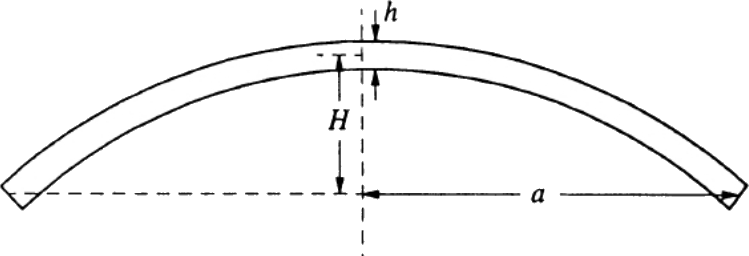
\includegraphics[width=0.9\linewidth]{00_Images/03_chapter/17.png}
%    \caption{Example mode shapes of a violin back plate}
%    \label{fig:violin_back_modes}
%\end{figure}

A key qualitative fact is that in wood typically \( E_L>E_R \). As a result, the mode families and degeneracies that are observed in a square isotropic plate do not generally occur in a square wood plate: the stiffness contrast along \( L \) and \( R \) breaks the symmetry between the two in-plane directions. To recover mode patterns analogous to the isotropic-square case one must choose a non-square aspect ratio satisfying
\[
\frac{L_x}{L_y} = \left(\frac{E_L}{E_R}\right)^{1/4}
\]
For Sitka spruce this gives approximately
\[
\frac{L_x}{L_y} \simeq 1.9
\]
In violin making, modes with patterns similar to the so-called x-mode and ring-mode are indeed observed on top and back plates and are used to tune plates before assembly. As an example reported for a violin back plate, mode shapes labeled 2 and 5 resemble x- and ring-like patterns (with indicative frequencies around 165 Hz and 350 Hz, respectively), alongside a lower mode around 85 Hz. 

\subsection{Simply Supported Orthotropic Plate: Modal Frequency Formula}

The frequency formulas derived for isotropic plates can be adapted to wood by replacing \( E \) with the appropriate directional modulus and replacing the isotropic Poisson combination \( \nu^{2} \) with the orthotropic product \( \nu_{xy}\nu_{yx} \). For a rectangular wood plate with simply supported edges, the \( (m,n) \) -th modal frequency is given as
\[
f_{mn}
 = 
0.453h
\left[
c_x\left(\frac{m+1}{L_x}\right)^{2}
+
c_y\left(\frac{n+1}{L_y}\right)^{2}
\right],
\qquad m,n = 0,1,2,\dots
\]
where the directional wave-speed-like parameters are
\[
c_x = \sqrt{\frac{E_x}{\rho\left(1-\nu_{xy}\nu_{yx}\right)}},
\qquad
c_y = \sqrt{\frac{E_y}{\rho\left(1-\nu_{yx}\nu_{xy}\right)}}
\]
In a quarter-cut plate one typically identifies \( x = L \) and \( y = R \), so that \( E_x = E_L \), \( E_y = E_R \) and the anisotropy enters explicitly through \( c_x\neq c_y \).

\section{Vibration in Shells}

\begin{figure}[!htb]
    \centering
    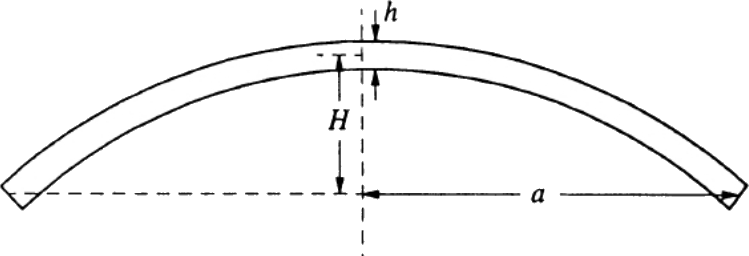
\includegraphics[width=0.9\linewidth]{00_Images/03_chapter/17.png}
    \caption{Effect of curvature on shell vibration and arching}
    \label{fig:shell_arching}
\end{figure}

Shells are thin curved surfaces. Compared with flat plates, curvature (arching) increases stiffness and has two immediate consequences in musical-acoustics structures:

\begin{enumerate}
    \item Static benefit arched parts can bear higher loads with less reinforcement. For example, the arched violin top plate can withstand string tension with only minor bracing (bass bar), while the flat guitar top plate typically requires substantial bracing to avoid yielding under the same type of load.
    \item Dynamic benefit: the vibrational response is modified: eigenfrequencies and mode families change because curvature couples bending and in-plane deformation.
\end{enumerate}

\subsection{Extensional vs Nonextensional Modes and Thickness Dependence}

Two limiting families of shell modes can be distinguished.

\begin{itemize}
    \item Extensional modes: vibrations that change the length of (at least) one line drawn on the shell surface. Their frequency is essentially independent of the thickness \( h \).
    \item Nonextensional modes: vibrations that do not change the length of any line on the shell (in the idealized sense). Their frequency is proportional to \( h \).
\end{itemize}

In practical shell geometries the separation is not always clean: modes may be partly extensional and partly nonextensional. A compact way to express this mixed dependence is
\[
f_{mn} = \left(A_{mn}+B_{mn}h^{2}\right)^{1/2}
\]
showing that thickness enters progressively (through the \( B_{mn}h^{2} \) term) rather than as an all-or-nothing classification.

\subsection{Spherical Shells: Lowest Axisymmetric Mode and Arching Effects}

Consider a spherical-cap shell of radius \( a \), thickness \( h \) and rise (depth) \( H \). When \( H = 0 \), the structure reduces to a flat circular plate and the lowest mode satisfies
\[
ka = \mu_0
\]
where \( \mu_0 \) depends on the boundary condition (as in the circular-plate formulas). When \( H\neq 0 \), curvature shifts the lowest mode so that approximately
\[
ka  \simeq \mu,
\qquad
\mu \approx
\begin{cases}
3, & \text{free edges or clamped edges with } H \text{ comparable to } h\\
6, & \text{clamped edges with } H \gg h
\end{cases}
\]

A more detailed prediction for the frequency of the lowest axisymmetric mode (displacement depending on \( r \) but not on \( \varphi \)) is given in normalized form as
\[
\frac{\omega}{\omega_0}
 = 
\left[
\frac{1}{1-\nu^{2}}\left(\frac{\mu}{\mu_0}\right)^{4}
+
\frac{48}{\mu_0^{4}}\left(\frac{H}{h}\right)^{2}
\right]^{1/2}
\]
where \( \omega_0 \) is the lowest-mode frequency of the flat circular plate with the same boundary conditions. This expression makes the role of arching explicit:

\begin{itemize}
    \item for a violin top plate, where the arching is typically a bit larger than the thickness, one finds approximately \( \omega  \simeq 2\omega_0 \);
    \item when \( H \ll h \), curvature is negligible and \( \omega \simeq \omega_0 \);
    \item for larger \( H/h \), it reports the asymptotic linear scalings
    \[
    \frac{\omega}{\omega_0} = 0.68\frac{H}{h}\quad \text{(clamped edges)},
    \qquad
    \frac{\omega}{\omega_0} = 0.84\frac{H}{h}\quad \text{(free edges)}
    \]
\end{itemize}

Finally, for a shell that is both thin and shallow (\( H/h\ge 20 \) and \( H/a<0.25 \)), the lowest frequency can be approximated directly by material and geometry
\[
\omega \simeq 2\left(\frac{E}{\rho}\right)^{1/2}\frac{H}{a^{2}}
\]

\subsection{Cylindrical Shells: Two Musical-Acoustics Applications}

Cylindrical shells appear in two relevant contexts. 

\begin{enumerate}
    \item Drum shells: the shell acts as a support structure for a light membrane. Two shell modes are especially important:
    \begin{itemize}
        \item a lowest extensional (breathing) mode, involving radial motion of the shell wall;
        \item a nonextensional mode involving ovalization (the cross-section becomes elliptical).
    \end{itemize}
    These become particularly relevant when the shell itself is excited by sticks.
    \item Orchestral chimes (tubular bells): tubes behave similarly to bars but with shape dependent corrections. It reports that bending-mode frequencies decrease when the cylinder is not perfectly rectilinear.
\end{enumerate}

\section{Driving-Point Impedance}

For continuous structures, the response to excitation depends not only on frequency but also on where the system is driven and where the motion is observed. A compact quantity that summarizes this dependence is the mechanical impedance, defined as the ratio between applied force and resulting velocity. 

\subsection{Definition and Measurement}

\begin{figure}[!htb]
    \centering
    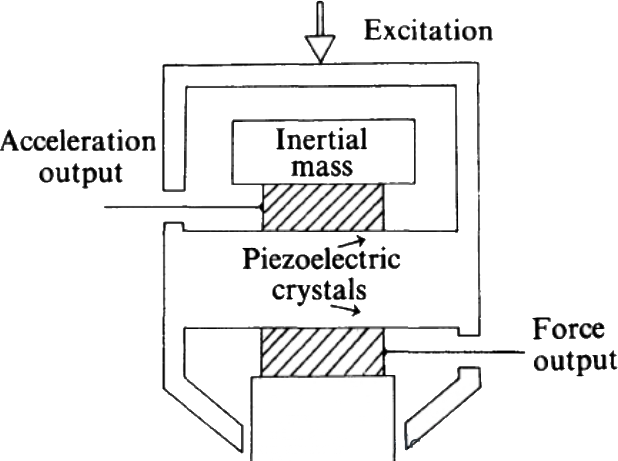
\includegraphics[width=0.7\linewidth]{00_Images/03_chapter/18.png}
    \caption{Impedance-head measurement of driving-point impedance}
    \label{fig:impedance_head}
\end{figure}

The (transfer) mechanical impedance between an excitation point \( \vv{r_F} \) and an observation point \( \vv{r_v} \) is
\[
Z(\omega;\vv{r_F},\vv{r_v}) = \frac{F(\omega;\vv{r_F})}{v(\omega;\vv{r_v})}
\]
In general, \( Z \) varies with the locations of the input and output points. A particularly important case is the driving-point (or input) impedance, obtained when force and velocity are measured at the same point:
\[
Z_{\mathrm{in}}(\omega;\vv{r_0}) = \frac{F(\omega;\vv{r_0})}{v(\omega;\vv{r_0})}
\]
Its reciprocal,
\[
Y_{\mathrm{in}}(\omega;\vv{r_0}) = \frac{1}{Z_{\mathrm{in}}(\omega;\vv{r_0})} = \frac{v(\omega;\vv{r_0})}{F(\omega;\vv{r_0})}
\]
is the driving-point admittance (mobility). 

\paragraph{Impedance head} A practical way to measure \( Z_{\mathrm{in}} \) is an impedance head, which combines a force sensor and an accelerometer (or velocity sensor) in one device. The head is attached to an electromagnetic shaker, which can generate pseudo-random sequences or swept-sine excitation. A crucial experimental detail is that the head has its own inertial mass \( m \), which loads the structure and therefore modifies the measured impedance if the attachment point is light.

\subsection{Infinite vs Finite Structures}

For an infinite structure there are no reflections, so the driving-point impedance is closely related to the characteristic wave impedance of the propagating wave.

\paragraph{Examples (infinite structures)} It lists the following relevant results. 

\begin{itemize}
    \item Longitudinal wave in an infinite bar:
    \[
    Z = \mu c_L
    \]
    where \( \mu \) is the mass per unit length and \( c_L \) is the longitudinal wave speed.
    \item Bending waves in an infinite bar:
    \[
    Z(f) = \mu v(f)\frac{1+j}{2}
    \]
    so the magnitude increases as \( \sqrt{f} \) (because the bending-wave phase velocity \( v(f) \propto \sqrt{f} \)).
    \item Infinite thin plate: the driving-point impedance is constant with frequency (a hallmark of 2D bending-wave spreading) and it can be written in terms of the bending stiffness
    \[
    D = \frac{E h^{3}}{12(1-\nu^{2})}
    \]
    as
    \[
    Z = 8\sqrt{\rho_sD}
    \qquad
    \left(\rho_s = \sigma = \rho h\ \text{mass per unit area}\right)
    \]
\end{itemize}

For finite structures, reflections from boundaries produce standing-wave resonances. As a result, the driving-point impedance (or admittance) shows sharp peaks and dips associated with the eigenmodes and the detailed curve depends strongly on the measurement point (nodal/antinodal location). This is illustrated by:

\begin{itemize}
    \item the driving-point impedance of a finite bar measured at an endpoint for different damping factors;
    \item the driving-point admittance of a finite plate measured at two different surface points, yielding visibly different resonance patterns.
\end{itemize}

\paragraph{Effect of damping} The damping factor is expressed as
\[
\frac{2\alpha}{\omega_0} = \frac{1}{Q}
\]
Increasing damping reduces the sharpness of resonance features: peaks are broader and lower and the impedance curve becomes smoother as the modal overlap increases.

\begin{figure}[!htb]
    \centering
    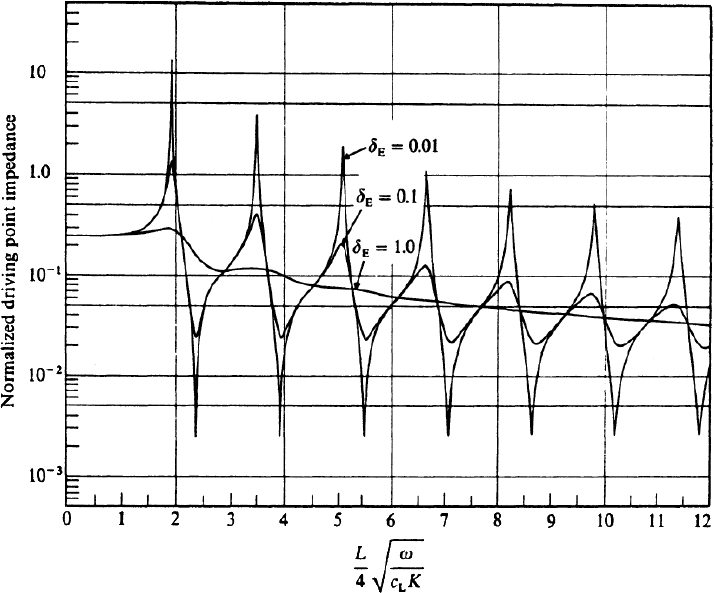
\includegraphics[width=0.75\linewidth]{00_Images/03_chapter/19.png}
    \caption{Driving-point impedance/admittance in finite structures}
    \label{fig:Driving_point_admittance}
\end{figure}

\section{Coupling Between Vibrating Systems}

When two vibrating structures can exchange vibrational energy, the behavior of the coupled assembly can differ significantly from the behavior of each structure in isolation. In musical instruments this situation is ubiquitous: a string drives a bridge, the bridge drives a soundboard, and the soundboard interacts with the enclosed air. The key point is that coupling is not just an ``energy leak'': if the coupled structure has its own resonances, it can shift or split the resonances of the driven structure. 

\subsection{Springlike and Masslike Terminations Around a Resonance}

As already encountered the special case of a string ended by a termination that is purely masslike or purely springlike, which systematically raises or lowers the resonance frequencies. The more general (and more realistic) case is when the termination itself is resonant (e.g. a bridge with its own modes). Then the termination impedance is frequency dependent and changes qualitative character across its resonance. In particular, denoting the termination impedance by \( Z_b(\omega) \), its imaginary part determines whether the termination behaves as a spring or a mass:
\[
\Im\{Z_b(\omega)\}<0 \quad\Rightarrow\quad \text{springlike behavior},
\qquad
\Im\{Z_b(\omega)\}>0 \quad\Rightarrow\quad \text{masslike behavior}
\]
For a bridge resonance close to a string resonance:

\begin{itemize}
    \item below the bridge resonance, the bridge appears springlike;
    \item above the bridge resonance, the bridge appears masslike.
\end{itemize}

As a consequence, the resonances of the string are pushed away from the bridge resonance and can be split into two nearby peaks: the coupled system reorganizes its modal structure.

\subsection{Weak vs Strong Coupling}

Coupling does not always produce a dramatic modification of the spectrum. Two regimes can be distinguished.

\paragraph{Weak coupling} The eigenfrequencies of the structure where the vibration is generated are essentially unaffected by the other structure. In this case, a sequential (one-way) approach is acceptable for vibroacoustic characterization:

\begin{itemize}
    \item compute the vibrational response of the first structure neglecting interaction;
    \item use that response as the excitation (initial condition / boundary input) for the second structure.
\end{itemize}

\paragraph{Strong coupling} The interaction modifies the eigenfrequencies of both structures. Then a sequential approach fails: one must solve the vibroacoustic response of the coupled system simultaneously (one set of equations with mutual interaction). The transition between weak and strong coupling depends on the properties of the two structures and, crucially, on frequency.

\section{Coupling Criteria}

The weak/strong coupling distinction becomes quantitative once one introduces dimensionless parameters comparing the characteristic impedances (and stored energy) of the interacting subsystems. This section summarizes two standard criteria from musical acoustics: coupling between a plate and the surrounding air, and coupling between a string and a soundboard.

\subsection{Coupling Between a Plate and Air}

A relevant example is a vibrating plate surrounded by air. In this case the weak/strong coupling regime is governed by the dimensionless parameter 
\[
\beta_c = \frac{\rho_0 c_0}{\rho_s h_s\,\omega_c}
\]
where

\begin{itemize}
    \item \( h_s \) is the plate thickness,
    \item \( \rho_s \) is the density of the structure (plate material),
    \item \( \rho_0 \) is the density of the fluid (air),
    \item \( c_0 \) is the sound speed in the fluid,
    \item \( \omega_c \) is the critical angular frequency of the plate, i.e. the frequency above which the plate can radiate sound efficiently.
\end{itemize}

The criterion reported in the slides is: 
\[
\beta_c  \ll 1 \quad \Rightarrow \quad \text{weak coupling},
\qquad
\beta_c \gtrsim 1 \quad \Rightarrow \quad \text{strong coupling}
\]
\paragraph{Remark} In this plate-air case, the slides explicitly note that the classification as weak/strong coupling does not depend on frequency (the relevant frequency scale is already embedded in \( \omega_c \)). 

\subsection{String Coupled to a Soundboard: Weak and Strong Coupling}

The coupling between a string and a soundboard can also be weak or strong. The slides express the regime in terms of the dimensionless ratio \( m/(n^2M) \), where:

\begin{itemize}
    \item \( m \) is the mass of the string,
    \item \( M \) is the effective mass of the soundboard (for the relevant resonance),
    \item \( n \) is the string mode number,
    \item \( Q_B \) is the merit factor (quality factor) of the soundboard resonance.
\end{itemize}

\begin{figure}[!htb]
    \centering
    \subfloat[Strong]{%
        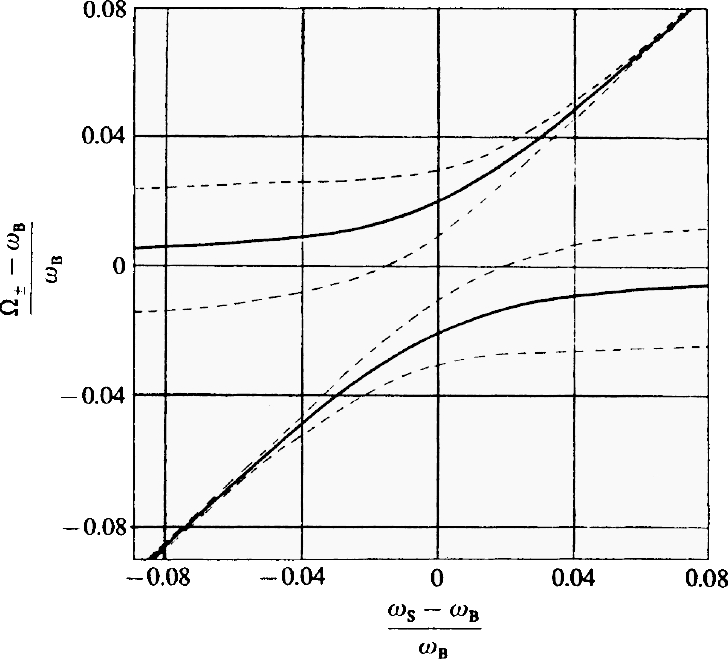
\includegraphics[height=0.25\textheight]{00_Images/03_chapter/21.png}%
    }\hfill
    \subfloat[Weak]{%
        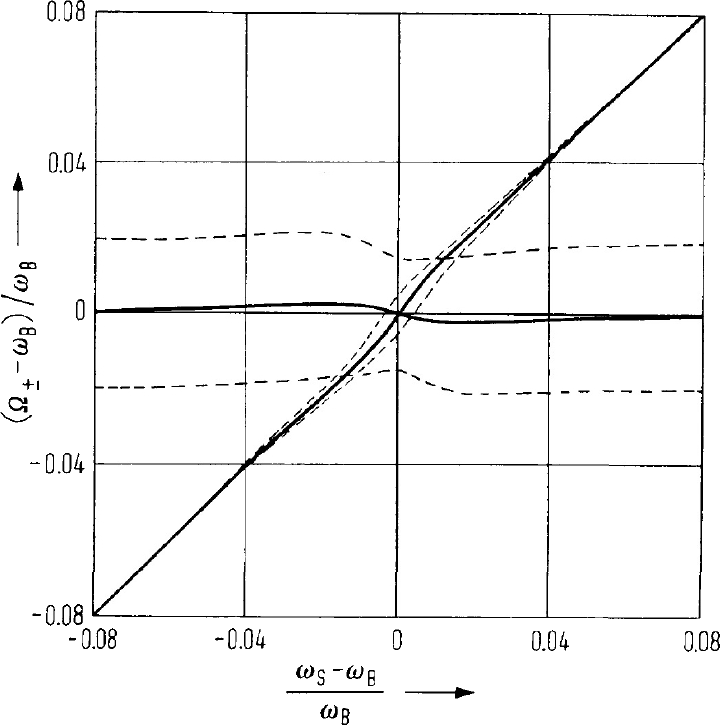
\includegraphics[height=0.25\textheight]{00_Images/03_chapter/22.png}%
    }
    \caption{Weak vs strong coupling between a string mode and a soundboard resonance}
    \label{fig:string_soundboard_coupling}
\end{figure}

\paragraph{Weak coupling} Weak coupling occurs when
\[
\frac{m}{n^{2}M}<\frac{\pi^{2}}{4Q_B^{2}}
\]
In this regime, if a string mode and a soundboard mode originally coincide in frequency, the coupling does not significantly alter their normal-mode frequencies. What changes instead is the damping: energy leakage into the soundboard modifies decay rates, while the resonance locations remain essentially those of the uncoupled subsystems.

\paragraph{Strong coupling and mode splitting} Strong coupling occurs when
\[
\frac{m}{n^{2}M}>\frac{\pi^{2}}{4Q_B^{2}}
\]
If the two uncoupled resonances coincide at \( \omega_0 \) (i.e. \( \omega_n = \omega_B = \omega_0 \)), the slides state that the normal modes are split symmetrically about \( \omega_0 \), and their damping factor becomes \( 2Q_B \).

\paragraph{Graphical interpretation} The plotted curves in the slides show that the normalized separation of the two coupled frequencies increases with \( m/(n^2M) \), and that the amount of splitting depends on \( Q_B \): higher- \( Q_B \) boards (sharper resonances) exhibit a more pronounced separation for the same mass ratio. A second plot summarizes the overall behavior by showing avoided crossing and symmetric splitting in the strong-coupling case and nearly unchanged resonance lines (but altered damping) in the weak-coupling case.

\section{Two Strings Coupled by a Bridge}

This configuration is relevant in string instruments whenever two strings are tuned at very close frequencies (a typical example is unison strings in the piano). We consider two strings that are identical in length \( L \), density \( \rho \), cross-sectional area \( S \), and linear density \( \mu = \rho S \), but differ in their tensions \( T_1 \) and \( T_2 \). Their transverse displacements are denoted \( y_1(x,t) \) and \( y_2(x,t) \).

\subsection{Governing Equations and Bridge Boundary Conditions}

\begin{figure}[!htb]
    \centering
    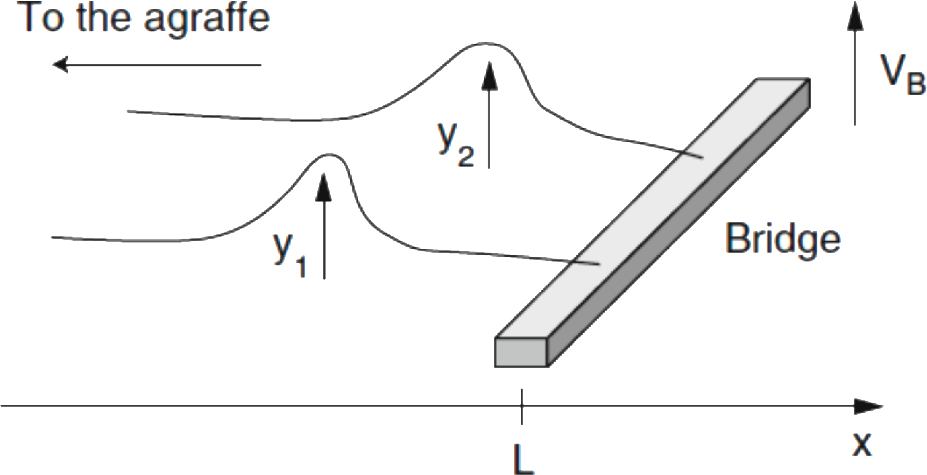
\includegraphics[width=0.8\linewidth]{00_Images/03_chapter/23.png}
    \caption{Two strings coupled by a bridge: schematic model}
    \label{fig:two_strings_bridge}
\end{figure}

Each string satisfies the (lossless) wave equation
\[
\left\{
\begin{aligned}
\rho S\,\frac{\partial^2 y_1}{\partial t^2}-T_1\,\frac{\partial^2 y_1}{\partial x^2}& = 0\\
\rho S\,\frac{\partial^2 y_2}{\partial t^2}-T_2\,\frac{\partial^2 y_2}{\partial x^2}& = 0
\end{aligned}
\right.
\]
The ends far from the bridge are fixed. At the bridge (\( x = L \)) the two strings share the same displacement,
\[
y_1(L,t) = y_2(L,t) = q_B(t)
\]
where \( q_B(t) \) is the bridge displacement. The bridge is characterized (in the frequency range of interest) by a mechanical impedance \( Z_B \), so that
\[
F_B(\omega) = Z_B(\omega)\,V_B(\omega),
\qquad
V_B = j\omega q_B
\]
The total force exerted by the two strings on the bridge is the sum of the end forces
\[
F_B = F_1+F_2
 = -T_1\left.\frac{\partial y_1}{\partial x}\right|_{x = L}
   -T_2\left.\frac{\partial y_2}{\partial x}\right|_{x = L}
\]

\subsection{Reduced Modal Model Near Unison}

The displacement of each string can be expanded onto its eigenmodes,
\[
y_1(x,t) = \sum_{n = 1}^{N}\phi_{1n}(x)\,q_{1n}(t),
\qquad
y_2(x,t) = \sum_{n = 1}^{N}\phi_{2n}(x)\,q_{2n}(t)
\]
For bridges with reduced mobility, the mode shapes remain close to the fixed-end shapes,
\[
\phi_{in}(x) \simeq \sin(k_n x),\qquad i = 1,2
\]
and the deviations from ideal fixed-end behavior are concentrated in the generalized coordinates \( q_{in}(t) \). Restricting attention to the fundamental modes gives
\[
y_1(x,t) \simeq \phi_1(x)\,q_1(t),\qquad
y_2(x,t) \simeq \phi_2(x)\,q_2(t)
\]
and we may write the two uncoupled oscillators schematically as
\[
\left\{
\begin{aligned}
\ddot{q}_1+\omega_1^2 q_1 & = g_1(q_i)\\
\ddot{q}_2+\omega_2^2 q_2 & = g_2(q_i)
\end{aligned}
\right.
\]
where the coupling effects are included in the perturbation terms \( g_i \). We seek complex-frequency solutions \( q_i(t) \propto e^{j\beta t} \) (with \( \beta \) complex to include attenuation), which leads to
\[
(\omega_0^2-\beta^2)\psi_1 = \gamma_1(\psi_i),
\qquad
(\omega_0^2-\beta^2)\psi_2 = \gamma_2(\psi_i)
\]
where \( \psi_i \) are complex amplitudes.
If detuning is small, the bridge impedance can be approximated as \( Z_B(\omega) \simeq Z_B(\omega_0) \), and it is convenient to work with the bridge admittance \( Y_B = 1/Z_B \). Using the end impedance of a string,
\[
Z = jZ_c\cot(kL)
\]
and expanding \( \cot(\cdot) \) around the fundamental, one obtains (near \( \omega_0 \)) a local relation between the end force and the bridge velocity. Specializing to the two strings yields the coupled system
\[
\left\{
\begin{aligned}
(\omega_1^2-\beta^2)F_1 & = -\frac{2T_1}{L}\,j\beta\,Y_B\,(F_1+F_2)\\
(\omega_2^2-\beta^2)F_2 & = -\frac{2T_2}{L}\,j\beta\,Y_B\,(F_1+F_2)
\end{aligned}
\right.
\]

\subsection{Detuning Parameter and Eigenvalues}

Let the two strings be slightly detuned by writing
\[
\omega_1 = \omega_0,
\qquad
\omega_2 = \omega_0(1+2\epsilon)
\]
which corresponds (to first order) to \( T_2 = T_1(1+4\epsilon) \).
With this parametrization, the coupled system can be reduced to
\[
\left\{
\begin{aligned}
j(\beta-\omega_0)F_1 & = j\zeta(F_1+F_2)\\
j(\beta-\omega_0)F_2 & = j\zeta(F_1+F_2)+2j\epsilon\omega_0 F_2
\end{aligned}
\right.
\]
where \( \zeta \) is a normalized coupling coefficient proportional to \( Y_B \).
Writing \( \beta = \omega_0+\alpha \) and introducing the dimensionless quantities
\[
a = \frac{\alpha}{\omega_0},\qquad \chi = \frac{\zeta}{\omega_0}
\]
one obtains the eigenproblem
\[
ja
\begin{bmatrix}
F_1\\F_2
\end{bmatrix}
 = 
j
\begin{bmatrix}
\chi & \chi\\
\chi & \chi+2\epsilon
\end{bmatrix}
\begin{bmatrix}
F_1\\F_2
\end{bmatrix}
\]
The eigenvalues \( a_\pm \) follow from
\[
a^{2}-2a(\chi+\epsilon)+2\epsilon\chi = 0
\qquad\Longrightarrow\qquad
a_\pm = \chi+\epsilon\pm\sqrt{\epsilon^{2}+\chi^{2}}
\]
The real part of \( a_\pm \) determines the eigenfrequency shift, while the imaginary part determines the damping factor.

\subsection{Reactive, Resistive, and Complex Bridge Admittance}

Different behaviors occur depending on the nature of the bridge admittance \( Y_B \), i.e. of \( \chi \).

\paragraph{Purely Reactive Admittance} If \( Y_B \) is purely reactive, then \( \chi = \xi\in\mathbb{R} \). The eigenfrequencies (real part of \( a_\pm \)) approach the uncoupled values when \( |\epsilon| \) is large, while in the unison limit \( \epsilon\to 0 \) the coupling becomes dominant and the two eigenfrequencies move apart (avoided crossing / splitting). Since \( \chi \) is real, no additional damping is introduced by the bridge in this idealized reactive case.

\paragraph{Purely Resistive Admittance} If \( Y_B \) is purely resistive, then \( \chi = j\eta \) with \( \eta>0 \). Two regimes arise:

\begin{itemize}
    \item If \( \epsilon>\eta \), then
    \[
    a_\pm = \epsilon+j\eta\pm\sqrt{\epsilon^{2}-\eta^{2}}
    \]
    so the eigenfrequency shifts (real parts) follow two hyperbola-like branches, while the damping (imaginary part) remains constant and equal to \( \eta \).
    \item If \( \eta>\epsilon \), the real part collapses to the line segment
    \[
    \Re\{a_\pm\} = \epsilon
    \]
    while the imaginary parts trace a circle in the complex plane (center at \( j\eta \), radius \( \eta \)), corresponding to a redistribution of damping between the two coupled modes.
\end{itemize}

\paragraph{Complex Admittance and Damping Redistribution} If \( Y_B \) is complex, \( \chi = \xi+j\eta \), an intermediate situation occurs. The coupling modifies eigenfrequencies and damping significantly only for sufficiently small detuning \( \epsilon \). A striking result in the unison limit (\( \epsilon = 0 \)) is that one of the two eigenmodes can become essentially undamped while the other becomes strongly damped: it is as if the bridge dissipation is pumped by one mode out of the two, leaving the other mode to survive for a much longer time.

\begin{figure}[!htb]
    \centering
    \subfloat[Real Part]{
        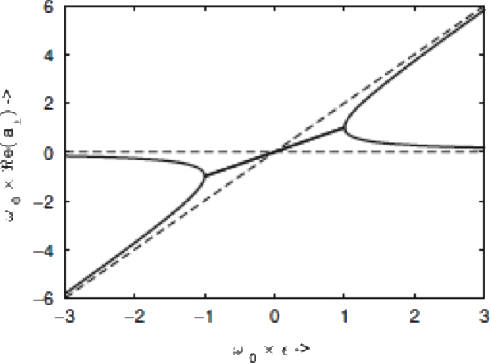
\includegraphics[height=0.2\textheight]{00_Images/03_chapter/24.png}
    }
    \hfill
    \subfloat[Immaginary Part]{
        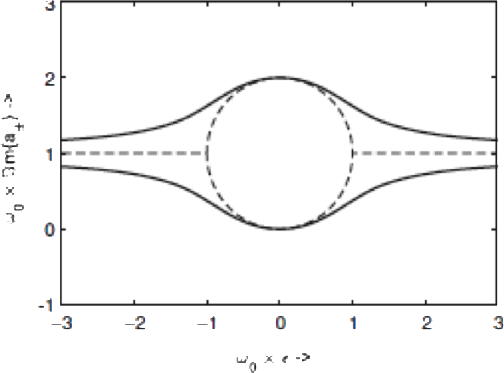
\includegraphics[height=0.2\textheight]{00_Images/03_chapter/25.png}
    }
    \caption{Bridge admittance}
    \label{fig:bridge_admittance_cases}
\end{figure}

\subsection{Time-Domain Interpretation}

\begin{figure}[!htb]
    \centering
    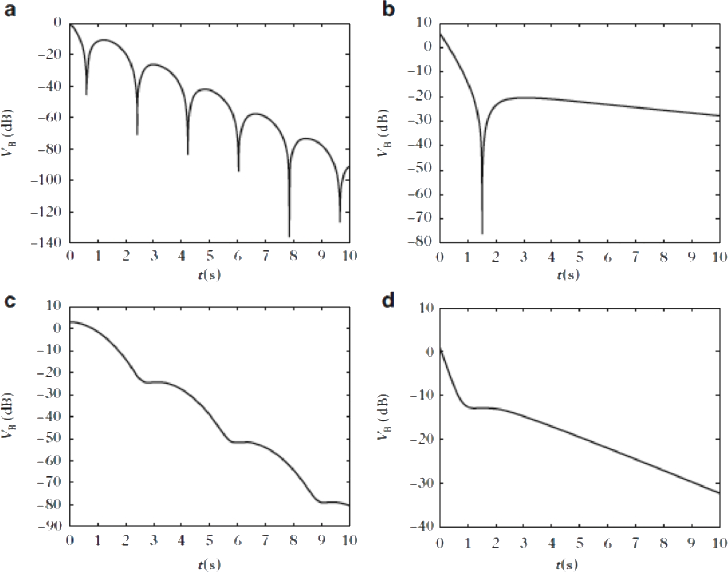
\includegraphics[width=0.85\linewidth]{00_Images/03_chapter/26.png}
    \caption{Time-domain responses for different coupling regimes}
    \label{fig:coupling_time_domain}
\end{figure}

Once \( F_1(t) \) and \( F_2(t) \) are reconstructed from the modal decay rates associated with \( a_{\pm} \), the bridge velocity is obtained as
\[
V_B = Y_B(F_1+F_2)
\]
The corresponding time responses can have very different envelopes. With mainly resistive coupling (large \( \eta \)) the decay is dominated by dissipation, while mainly reactive coupling (large \( \xi \)) tends to emphasize beating. For a genuinely complex admittance, it is common to observe an uneven redistribution of damping: one component decays quickly, leaving a slowly decaying residual motion linked to the weakly damped coupled mode.

\section{Nonlinear Effects in Shells and Plates}

Up to now, the governing equations have been treated as linear, so that mode shapes and eigenfrequencies are independent of vibration amplitude. In real plates and shells this assumption can break down when the deflection becomes large compared to the thickness (or to the shell curvature depth). In that case, geometric nonlinearities introduce an amplitude-dependent stiffness, and therefore the modal frequencies are no longer constant.

\begin{figure}[!htb]
    \centering
    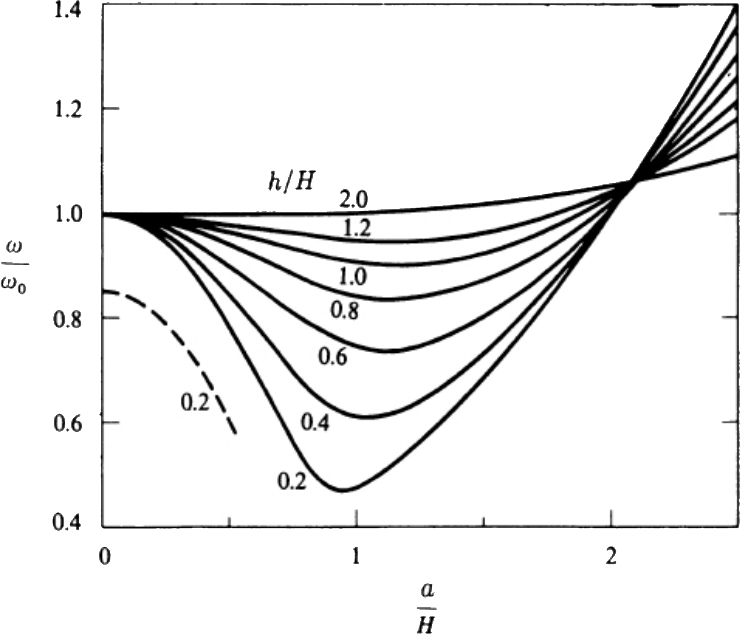
\includegraphics[width=0.6\linewidth]{00_Images/03_chapter/27.png}
    \caption{Typical nonlinear frequency shift in plates/shells with increasing amplitude}
    \label{fig:nonlinear_shift}
\end{figure}

\subsection{Amplitude-Dependent Frequency in a Circular Plate}

A simple (and very useful) rule of thumb is given for a flat circular plate of thickness \( h \), vibrating with displacement amplitude \( a \). The oscillation frequency increases with amplitude according to the approximation
\[
\omega  \approx \omega_0\left[1 + 0.16\left(\frac{a}{h}\right)^2\right]
\]
where \( \omega_0 \) is the small-amplitude (infinitesimal) angular frequency. This effect is especially relevant in instruments such as gongs, where vibration amplitudes can be large enough that audible pitch glide occurs during the decay.

\subsection{Nonlinear Behavior in Shells}

For shells the picture becomes more complex because the curvature couples bending and in-plane stretching. The slides summarize the behavior in terms of the frequency ratio \( \omega/\omega_0 \) as a function of the normalized amplitude \( a/H \), where \( H \) is the cap height, and for different values of the thickness ratio \( h/H \).

\paragraph{Thin shells: tension-dominated nonlinearity} If the shell is very thin, \( h/H  \ll 1 \), nonlinear tension effects dominate the response. As the vibration amplitude increases towards the shell depth (\( a \to H \)), the mode frequency can drop to about half of its small-amplitude value. A further increase in amplitude causes the frequency to rise again. 

\paragraph{Thicker shells: bending-dominated response} As the ratio \( h/H \) increases, bending stiffness becomes more important and the nonlinear effect weakens. The ratio \( \omega/\omega_0 \) stays closer to unity, and the frequency shift with amplitude becomes less evident.


    %! TEX root = main.tex

\chapter{Sound Propagation}

This chapter analyzes how sound waves propagate in the environment. It isn't concerned with the generation mechanism, but only with propagation in the surrounding medium. Sound can be described as a perturbation of the air pressure field with frequency content in the range \SIrange{20}{20000}{\hertz}.

\section{Equation of Air Motion and Plane Waves}

Considering one-dimensional propagation along the \( x \) axis, the pressure perturbation \( p(x,t) \) satisfies
\[
\frac{\partial^{2} p}{\partial t^{2}} = c^{2} \frac{\partial^{2} p}{\partial x^{2}}
\]
where \( c \) is the sound speed. Under small-signal adiabatic conditions, the sound speed in air can be expressed as
\[
c = \sqrt{\frac{\gamma p_{a}}{\rho}}
\]
where \( \gamma \) is the ratio of specific heats, \( p_{a} \) is the ambient pressure, and \( \rho \) is the air density. A commonly used approximation highlights the dependence of \( c \) on temperature
\[
c = 331.3 + 0.606 \Delta T~\si{\metre\per\second}
\]
where \( \Delta T \) is the temperature in Celsius degrees. A general solution can be written as the superposition of two counter-propagating plane waves
\[
p(x,t) = A e^{-j k x} e^{j \omega t} + B e^{j k x} e^{j \omega t}
\]
where \( A \) and \( B \) are complex amplitudes and the wavenumber is \( k = \omega / c \). The particle velocity \( u(x,t) \) is the speed of air particles subject to the pressure perturbation \( p \). In free field, for a single progressive plane wave traveling in \( +x \) (i.e. \( B = 0 \)), where boundaries are absent, pressure and particle velocity are related by
\[
p = \rho c u
\]
This motivates the definition of wave impedance (also known as acoustic impedance)
\[
z = \frac{p}{u}
\]
For a plane wave, \( z = \rho c \), therefore its value does not depend on the measurement point.

\section{Spherical Waves}

When propagation occurs in three dimensions, the acoustic pressure \( p(x,t) \) satisfies the wave equation
\[
\frac{\partial^{2} p}{\partial t^{2}} = c^{2} \nabla^{2} p
\]
where \( \nabla^{2} \) is the Laplace operator. In Cartesian coordinates,
\[
\nabla^{2} p = \frac{\partial^{2} p}{\partial x^{2}} + \frac{\partial^{2} p}{\partial y^{2}} + \frac{\partial^{2} p}{\partial z^{2}}
\]
The wave equation reduces to the Helmholtz equation, assuming a time-harmonic behavior \( p(x,t) \propto e^{j \omega t} \)
\[
\nabla^{2} p + k^{2} p = 0
\]
with \( k = \omega / c \). In spherical coordinates, a general radially symmetric solution can be written as
\[
p(r,t) = \left( \frac{A}{r} e^{-j k r} + \frac{B}{r} e^{j k r} \right) e^{j \omega t}
\]
where \( A \) and \( B \) are the amplitudes of the outgoing and ingoing spherical waves, respectively. The particle velocity \( u(r,t) \) follows from the Euler equation
\[
\rho \frac{\partial u}{\partial t} = -\nabla p = -\frac{\partial p}{\partial r}
\]
If only the outgoing component is present (\(B=0\)),
\[
p(r,t) = \frac{A}{r}e^{-jkr} e^{j\omega t},
\qquad
u(r,t) = \frac{p(r,t)}{\rho c}\left(1 + \frac{1}{jkr}\right)
\]
and therefore
\[
z(r)=\frac{p}{u}=\rho c\left(\frac{jkr}{1 + jkr}\right)
\]
Two limiting regimes are of practical interest. For \( k r \gg 1 \),
\[
z \simeq \rho c
\]
so the spherical wave impedance approaches that of a plane wave. For \( k r \ll 1 \),
\[
z \simeq j \rho c k r
\]
and the impedance becomes purely imaginary.

\section{Sound Pressure Level and Intensity Level}

In many acoustics applications it is convenient to express pressure and intensity quantities on a logarithmic scale. This choice is motivated by the very large dynamic range of the human ear, spanning roughly six orders of magnitude between the minimum audible pressure and the maximum acceptable level. Given an acoustic pressure amplitude \( p_{\mathrm{rms}} \), the SPL is defined as
\[
L_p = 20\log_{10}\left(\frac{p_{\mathrm{rms}}}{p_0}\right)
\]
with \( p_{0} = \SI{20}{\micro\pascal} \) (rms in air) is taken as the minimum audible pressure around \SIrange{1}{3}{\kilo\hertz}. The sensitivity of the human ear is not constant with frequency, and it is maximal in the \SIrange{1}{3}{\kilo\hertz} region. A practical way to account for this effect is to apply a frequency weighting filter before computing the level, leading for instance to the dB(A) scale. A more general representation of frequency-dependent sensitivity is provided by the equal loudness curves, which specify the amplification that a stimulus at a given frequency requires in order to be perceived as equally loud as a reference tone at \SI{1}{\kilo\hertz}. Families of curves (figure \ref{fig:equal_loudness}) are reported for different SPL values of the stimulus.

\begin{figure}[!htb]
    \centering
    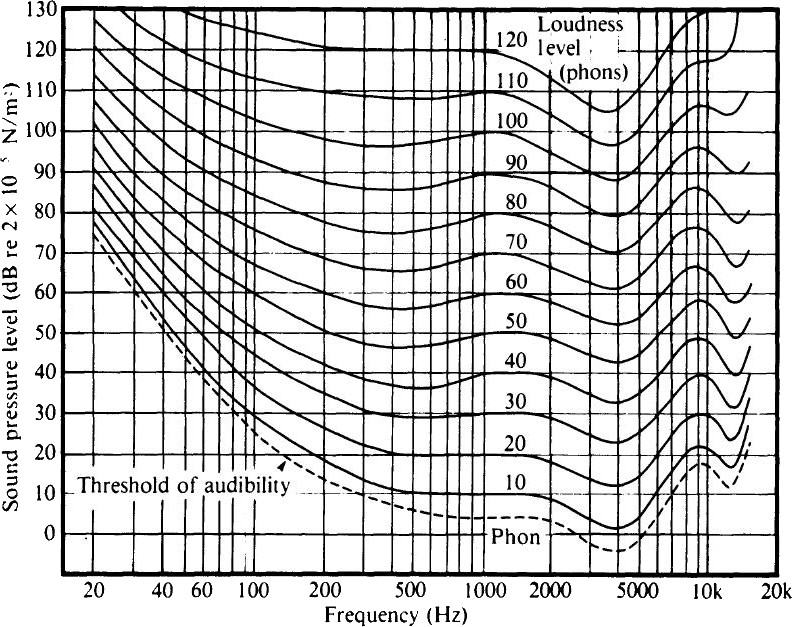
\includegraphics[width=0.6\linewidth]{00_Images/04_chapter/01.png}
    \caption{Equal-loudness contours of human hearing}
    \label{fig:equal_loudness}
\end{figure}

A second logarithmic measure concerns the energy transported by sound waves. The intensity level (IL) is defined as
\[
IL = 10 \log_{10}\left(\frac{I}{I_{0}}\right)
\]
where \( I \) is the acoustic intensity, measured in \si{\watt\per\square\metre}, and \( I_{0} = \SI{1e-12}{\watt\per\square\metre} \) is the conventional reference. For a progressive plane wave, using rms quantities, intensity can be related to acoustic pressure through
\[
I = \frac{p_{\mathrm{rms}}^2}{\rho c} = p_{\mathrm{rms}}u_{\mathrm{rms}}
\]
It is possible to observe cases where the SPL is large while the net intensity becomes negligible, for instance when energy fluxes in opposite directions balance each other (if peak amplitudes are used instead, the time-average intensity is smaller by a factor \( 1/2 \).)

\section{Normal Modes in Enclosures}

Let us consider an enclosure with a regular shape and focus on determining its normal modes. As a representative example, we take a rectangular cavity with dimensions \( a \), \( b \), and \( c \) along the three Cartesian axes. The acoustic pressure \( p(x,y,z,t) \) inside the cavity satisfies the three-dimensional wave equation
\[
\frac{\partial^{2} p}{\partial t^{2}} = c^{2}\left(\frac{\partial^{2} p}{\partial x^{2}} + \frac{\partial^{2} p}{\partial y^{2}} + \frac{\partial^{2} p}{\partial z^{2}}\right)
\]
The boundary condition at the walls can be expressed in terms of the wall acoustic impedance \( z_{w} \). Writing the pressure as \( p = z_{w} u \) and using the linear momentum equation in the frequency domain, one obtains
\[
p = z_{w} u = \frac{j z_{w}}{\rho \omega}\frac{\partial p}{\partial n}
\]
where \( \partial p / \partial n \) denotes the derivative along the outward normal to the surface. A particularly important case is that of rigid walls, for which \( z_{w} \to \infty \). In this limit the normal particle velocity vanishes, and the boundary condition becomes
\[
\frac{\partial p}{\partial n} = 0
\]
Under this assumption, a separable solution is
\[
p_{lmn}(x,y,z,t) = A \cos\left(\frac{l \pi x}{a}\right)\cos\left(\frac{m \pi y}{b}\right)\cos\left(\frac{n \pi z}{c}\right)\sin(\omega t)
\]
with \( l \), \( m \), \( n = 0,1,2,\dots \) and amplitude \( A \). The corresponding modal angular frequencies are
\[
\omega_{lmn} = \pi c\left(\frac{l^{2}}{a^{2}} + \frac{m^{2}}{b^{2}} + \frac{n^{2}}{c^{2}}\right)^{1/2}
\]
The distribution of modal frequencies depends strongly on the cavity dimension ratios. For equal ratios, multiple modes may cluster and produce pronounced coincidences, whereas more incommensurate ratios lead to a more uniform spacing, as illustrated by the mode-density plots for \( 2:2:2 \) and \( 1:2:3 \). The influence of the enclosure proportions on the modal distribution is illustrated in figure \ref{fig:mode_distribution}, comparing a cubic-like cavity with a more incommensurate set of side ratios.

\begin{figure}[!htb]
    \centering
    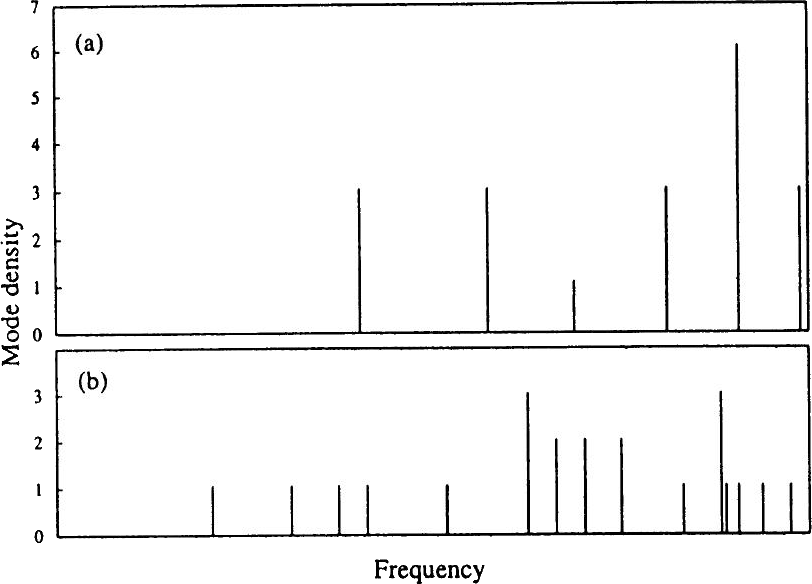
\includegraphics[width=0.6\linewidth]{00_Images/04_chapter/02.png}
    \caption{Mode distribution in a rectangular cavity for different side ratios}
    \label{fig:mode_distribution}
\end{figure}

    %! TEX root = main.tex

\chapter{Sound Radiation}

This chapter focuses on the radiation of sound from vibrating sources into an unbounded acoustic medium. The objective is to relate the source motion to the radiated pressure field and to quantify how efficiently acoustic power is transferred to the surrounding air. We start from elementary source models, which provide useful scaling laws with frequency and clarify the role of directivity in the radiated field. 

\section{Simple Multipole Sources}

\subsection{Monopole Source} 

A monopole can be modeled as a small spherical source of radius \( a \) pulsating at angular frequency \( \omega \). Its acoustic volume flow is
\[
Q = 4\pi a^{2} v(a)
\]
where \( v(a) \) is the normal velocity at the source surface. For \( ka \ll 1 \), the pressure at distance \( r \) from the source is
\[
p(r) = \frac{j\omega\rho}{4\pi r} Q e^{-jkr}
\]
The radiated acoustic power is obtained from the intensity integrated over a spherical surface \( S \)
\[
P = \int_{S}\frac{p^{2}}{\rho c} dS = \frac{\omega^{2}\rho Q^{2}}{8\pi c}
\]
Therefore the radiated power scales with \( \omega^{2} \). 

\subsection{Dipole Source} 

\begin{figure}[!htb]
    \centering
    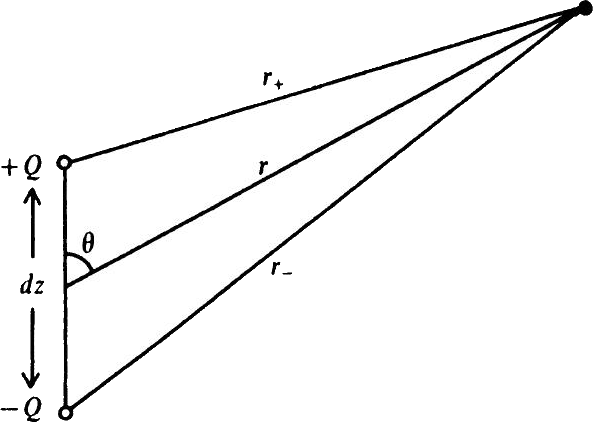
\includegraphics[width=0.6\linewidth]{00_Images/05_chapter/01.png}
    \caption{Dipole geometry and observation angle \(\theta\)}
    \label{fig:dipole_geom}
\end{figure}

A dipole is defined as two spherical sources of strength \( \pm Q \) separated by a distance \( dz \) that tends to zero. The pressure at \( (r,\theta) \) can be written as following, figure \ref{fig:dipole_geom} summarizes the geometry.
\[
p(r,\theta) = \frac{j\omega\rho}{4\pi}\left(\frac{e^{-jkr_{+}}}{r_{+}} - \frac{e^{-jkr_{-}}}{r_{-}}\right)Q
\]
If \( dz \to 0 \) and \( Q \to \infty \) while keeping \( \mu = Qdz \) finite, one obtains
\[
p(r,\theta) = \frac{\omega^{2}\rho}{4\pi c r}\left(1 + \frac{1}{jkr}\right)e^{-jkr}\mu\cos\theta
\]
The corresponding radiated power is
\[
P = \frac{\omega^{4}\rho\mu^{2}}{24\pi c^{3}}
\]
showing a \( \omega^{4} \) dependence, which makes dipole radiation much less efficient than monopole radiation at low frequencies.

\subsection{Quadripole Source} 

A quadripole field can be generated by combining dipole sources, as shown in figure \ref{fig:quadrupole_geom}, leading to a pressure of the form
\[
p_{q} = -jk^{3}\left(\frac{\rho c Q dz dx}{4\pi r}\right)\cos(\vv{r},\mathbf{z})\cos(\vv{r},\mathbf{x})e^{-jkr}
\]

\begin{figure}[!htb]
    \centering
    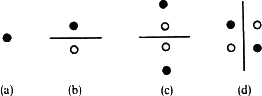
\includegraphics[width=0.8\linewidth]{00_Images/05_chapter/02.png}
    \caption{Quadrupole source as a combination of dipoles}
    \label{fig:quadrupole_geom}
\end{figure}

As the source order increases, the angular dependence becomes more complex and the low-frequency radiation efficiency decreases markedly compared to lower-order sources.

\section{Distribution of Point Sources}

The radiation pattern of an extended source can be understood by combining elementary point-like radiators with prescribed relative phases. In the following, \( Q \) denotes the acoustic volume flow associated with each point source and \( r \) is the distance to the observation point, with \( r \gg d \).

\subsection{Two Point-Like Sources} 

\begin{figure}[!htb]
    \centering
    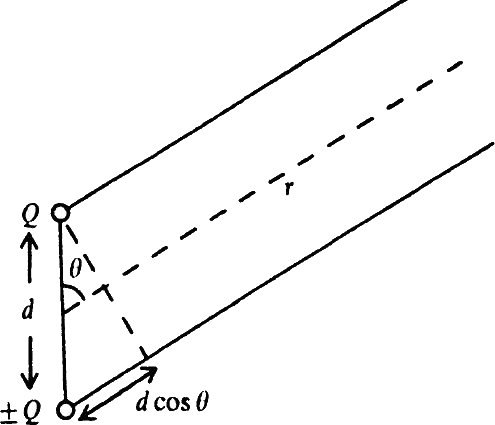
\includegraphics[width=0.5\linewidth]{00_Images/05_chapter/03.png}
    \caption{Geometry for two point-like sources separated by \(d\)}
    \label{fig:two_sources_geom}
\end{figure}

Consider two sources separated by a distance \( d \) and an angle \( \theta \), as illustrated in figure \ref{fig:two_sources_geom}. In the far field, the pressure can be approximated as
\[
p \approx \left(\frac{j\omega\rho Q}{4\pi r}\right)e^{-jkr}\left(e^{\frac{1}{2}jkd\cos\theta} \pm e^{-\frac{1}{2}jkd\cos\theta}\right)
\]
where the sign \( + \) corresponds to in-phase sources, while \( - \) corresponds to opposite-sign sources. The interference term introduces strong angular variations as \( kd \) increases. The radiated power is
\[
P = \frac{\omega^{2}\rho Q^{2}}{4\pi c}\left(1 \pm \frac{\sin(kd)}{kd}\right)^{2}
\]
Three limiting regimes are of interest. If \( kd \simeq 1 \), the pressure tends to vanish for several angles \( \theta \). If \( kd \ll 1 \), the power goes to zero for opposite-sign sources, while it becomes four times the power of a single monopole with strength \( Q \) in the in-phase case. If \( kd \gg 1 \), the power converges to twice the monopole power. The dependence of the radiated power on the non-dimensional spacing \(kd\) is shown in figure \ref{fig:two_sources_interf}.

\begin{figure}[!htb]
    \centering
    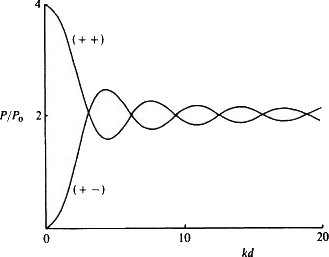
\includegraphics[width=0.6\linewidth]{00_Images/05_chapter/04.png}
    \caption{Interference effects for two point sources as a function of \(kd\)}
    \label{fig:two_sources_interf}
\end{figure}

\subsection{Line of 2N Sources} 

Consider a linear distribution of \( 2N \) sources at spacing \( d \), either all in phase or with alternating signs. The far-field pressure can be written as
\[
p_{\pm} \approx \frac{j\omega\rho Q}{4\pi r}e^{-jkr}\sum_{n=1}^{N}\pm(-1)^{n}\left[e^{(n-\frac{1}{2})jkd\cos\theta} \pm e^{(-n-\frac{1}{2})jkd\cos\theta}\right]
\]
For a co-phase array the expression reduces to
\[
p_{+} \approx \frac{j\omega\rho Q}{4\pi r}e^{-jkr}\frac{\sin(Nkd\cos\theta)}{\sin\left(\frac{1}{2}kd\cos\theta\right)}
\]
At broadside, \( \theta = 90^{\circ} \), the pressure tends to that of a single point source of strength \( 2NQ \) placed at the array center. The main lobe width scales as \( 2\pi/(Nkd) \). If \( d > \lambda/2 \), additional maxima appear at angles \( \theta^{\ast} = \cos^{-1}(2n\pi/(kd)) \). At high frequency the total radiated power is \( NP_{0} \), while at low frequency it is \( N^{2}P_{0} \), with \( P_{0} \) the power of one source.

\subsection{Antiphase Array} 

For alternating signs, the pressure can be written as
\[
p_{-}(r,\theta,t) \approx \left(\frac{j\omega\rho Q}{4\pi r}\right)e^{-jkr}\sum_{n=1}^{N}(-1)^{n}2j\sin\left(\left(n-\frac{1}{2}\right)kd\cos\theta\right)e^{j\omega t}
\]
or equivalently
\[
p_{-}(r,\theta,t) \approx \left(\frac{j\omega\rho Q}{4\pi r}\right)e^{-jkr}\left[\frac{(-1)^{N}\sin(Nkd\cos\theta)}{\cos\left(\frac{1}{2}kd\cos\theta\right)}\right]e^{j\omega t}
\]
An antiphase array is less efficient because the acoustic flow tends to remain internal to the array, reducing the energy escaping to the far field. At low frequency, \( \lambda > 2d \), the radiation efficiency approaches that of a single monopole source. At high frequency, \( \lambda < 2d \), maxima occur at \( \theta^{\ast} = \cos^{-1}((2n-1)\pi/(kd)) \). The evolution of the radiation pattern with the number of sources and with phase relation is illustrated in figure \ref{fig:line_arrays}.

\begin{figure}[!htb]
    \centering
    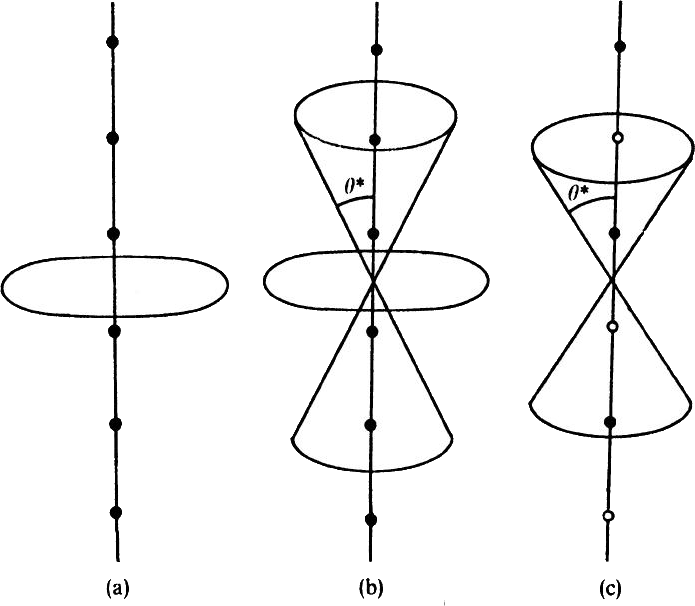
\includegraphics[width=0.6\linewidth]{00_Images/05_chapter/05.png}
    \caption{Radiation patterns of line arrays (in-phase and antiphase cases)}
    \label{fig:line_arrays}
\end{figure}

\section{Radiation from a Spherical Source}

In the previous discussion the radiating element was assumed to be acoustically compact, namely \( ka \ll 1 \). We now remove this constraint and consider a pulsating sphere of radius \( a \), whose normal surface velocity is \( u e^{j\omega t} \). The acoustic pressure at distance \( r \) from the center can be written as
\[
p(r,t) = j c \rho \frac{a^{2} k u}{r}\left(\frac{1 - jka}{1 + k^{2}a^{2}}\right)e^{-jk(r-a)}e^{j\omega t}
\]
The total radiated power follows from integrating the intensity over a spherical surface
\[
P = 2\pi \rho c \frac{k^{2}a^{4}u^{2}}{1 + k^{2}a^{2}}
\]
Two limiting cases clarify the frequency dependence. For \( ka \gg 1 \),
\[
P = 2\pi \rho c a^{2}u^{2}
\]
so the radiated power no longer increases with frequency. For \( ka \ll 1 \),
\[
P = 2\pi \rho c (ka)^{2} a^{2}u^{2}
\]
therefore the radiated power increases with frequency. Since most musical instruments operate with \( ka < 1 \), increasing the effective size of the radiating surface is advantageous at low frequency. The acoustic field exerts a mechanical load on the source surface. Let \( S = 4\pi a^{2} \) be the sphere area. The resulting force is
\[
F = 4\pi a^{2}p(a)
\]
and it can be expressed as
\[
F = \left(\rho c S \frac{k^{2}a^{2}}{1 + k^{2}a^{2}} + j\rho c S \frac{ka}{1 + k^{2}a^{2}}\right)u = (R_{m} + jX_{m})u
\]
The term \( R_{m}u \) represents the dissipative radiation load. It increases as \( (ka)^{2} \) at low frequency and then saturates. The term \( X_{m}u \) represents the mass load associated with the co-moving air. It grows approximately as \( ka \) for \( ka < 1 \) and then decreases as \( (ka)^{-1} \) for \( ka > 1 \). As a consequence, \( X_{m}u \) dominates at low frequency, whereas \( R_{m}u \) dominates at high frequency. Typical trends of the radiation resistance \(R_m\) and reactance \(X_m\) for a pulsating sphere are shown in figure \ref{fig:sphere_load}.

\begin{figure}[!htb]
    \centering
    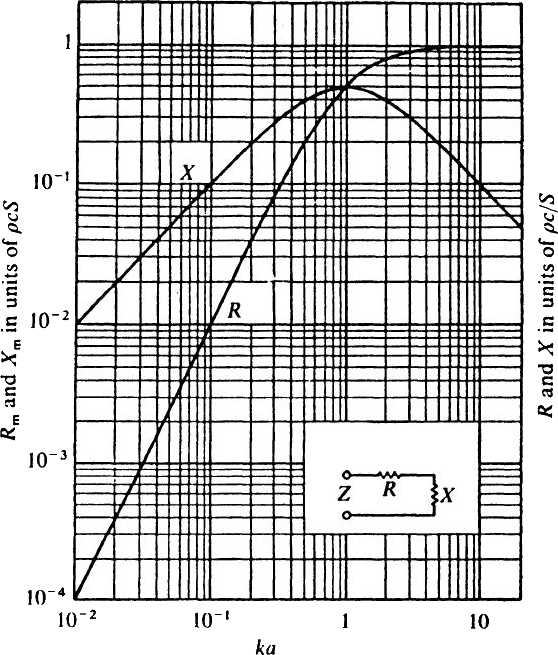
\includegraphics[width=0.5\linewidth]{00_Images/05_chapter/06.png}
    \caption{Radiation resistance and reactance of a pulsating sphere versus \(ka\)}
    \label{fig:sphere_load}
\end{figure}


\section{Strings as an Extreme Case of Line Sources}

Linear radiators provide a useful model for vibrating strings. We consider a cylindrical source of radius \( a \) oscillating at angular frequency \( \omega \), and we assume a small radius such that \( ka \ll 1 \). Let \( u e^{j\omega t} \) be the vibration velocity. In the far field, the acoustic intensity at distance \( r \) takes the form
\[
I \approx \left(\frac{\pi \rho \omega^{3} a^{2} u^{2}}{4 c^{2} r}\right)\cos^{2}\phi
\]
where \( \phi \) is the observation angle with respect to the source axis. The total radiated power is then
\[
P \approx \frac{\rho \pi^{2} \omega^{2} a^{4} u^{2}}{4 c^{2}}
\]
This expression shows a very strong dependence on both \( \omega \) and \( a \). In particular, for the strings encountered in musical instruments the radius is extremely small, and the resulting radiated power is therefore negligible compared to the radiation from larger vibrating surfaces. 

\section{Radiation from Baffled Plane Sources}

\begin{figure}[!htb]
    \centering
    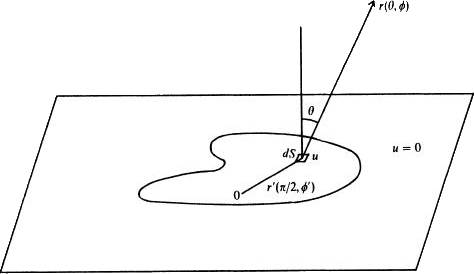
\includegraphics[width=0.7\linewidth]{00_Images/05_chapter/07.png}
    \caption{Geometry for radiation from a baffled plane source (Rayleigh integral)}
    \label{fig:rayleigh_geom}
\end{figure}

A widely used idealization for vibrating plates and membranes is a plane source mounted in an infinite rigid baffle. The source surface is described by coordinates \( \vv{r}' \), while the acoustic pressure is evaluated at an observation point \( \vv{r} \) with \( |\vv{r}| \gg |\vv{r}'| \) (the geometry is shown in figure \ref{fig:rayleigh_geom}). The infinitesimal contribution of a surface element \( dS \) vibrating with normal velocity \( u(\vv{r}') \) is
\[
dp(\vv{r}) = \frac{j\omega\rho}{2\pi r} e^{-jk|\vv{r}-\vv{r}'|} u(\vv{r}') dS
\]
Integrating over the entire radiating surface \( S \) yields, in the far field,
\[
p(r,\theta,\phi) = \frac{j\omega\rho}{2\pi r} e^{-jkr} \iint_{S} e^{jkr'\sin\theta\cos(\phi-\phi')} u(r') r' d\phi' dr'
\]
The pressure field is therefore proportional to the spatial Fourier transform of the surface velocity distribution.

\subsection{Circular Piston} 

Consider a circular piston of radius \( a \) vibrating with uniform normal velocity \( u \). The far-field pressure can be written as
\[
p \approx \frac{1}{2} j\omega\rho u a^{2} \frac{e^{-jkr}}{r}\left[\frac{2J_{1}(ka\sin\theta)}{ka\sin\theta}\right]
\]
For \( ka \ll 1 \) the directivity factor tends to one and
\[
p \approx \frac{1}{2} j\omega\rho u a^{2} \frac{e^{-jkr}}{r}
\]
so the source is approximately isotropic. As frequency increases, the first zero of \( J_{1} \) implies a radiation null at
\[
\theta^{\ast} = \sin^{-1}\left(\frac{3.83}{ka}\right)
\]
highlighting the progressive narrowing of the main lobe.

\subsection{Non-uniform Velocity Distributions} 

If the velocity is not constant over the surface, as for membranes vibrating in higher modes, nodal lines and nodal circles imply regions of opposite sign. A cross flow is required to sustain these patterns, and the associated cancellation makes such modes inefficient radiators, similarly to arrays with alternating signs. The most effective membrane modes are the axisymmetric ones, which have a monopole rather than a dipole character. 

\subsection{Mechanical Load on the Piston} 

The acoustic field exerts a load on the source that can be written as
\[
F = (R_{m} + jX_{m})u = \rho c S u (A + jB)
\]
where \( S \) is the piston area. The coefficients are
\[
A = 1 - \frac{J_{1}(2ka)}{ka}
\]
\[
B = \frac{H_{1}(2ka)}{ka}
\]
with \( J_{1} \) the Bessel function and \( H_{1} \) the Struve function. Their limiting behaviors are
\[
A \to \frac{1}{2}(ka)^{2} \quad ka \ll 1
\]
\[
A \to 1 \quad ka \gg 1
\]
\[
B \to \frac{8ka}{3\pi} \quad ka \ll 1
\]
\[
B \to \frac{2}{\pi ka} \quad ka \gg 1
\]
These trends are consistent with the frequency dependence previously observed for the mechanical radiation load of a pulsating sphere. 

\section{Unbaffled Radiators}

Only a limited number of musical instruments can be idealized as sources mounted in an infinite rigid baffle. In practice, most radiating surfaces are unbaffled, and therefore radiate into the full space, over a solid angle \( 4\pi \) rather than \( 2\pi \). A direct consequence concerns the radiated power at low frequency. When \( ka < 1 \), the absence of the baffle reduces the radiated power by approximately a factor \( 2 \) compared to the baffled case. At high frequency, the directional behavior is essentially unchanged with respect to a baffled radiator. As a result, the spectrum of the radiated signal from an unbaffled source is shifted towards higher frequencies compared to the baffled case. A useful characterization is provided by the mechanical radiation resistance of an unbaffled piston. In the low-frequency range, for \( ka < 2 \),
\[
R_{m} \approx 3 \times 10^{-2}\rho c S (ka)^{4}
\]
while for \( ka > 3 \),
\[
R_{m} \approx \rho c S
\]
In the regime \( ka < 2 \), most of the radiation is suppressed, consistently with the strong reduction of radiated power for unbaffled sources at low frequency. 

\section{Radiation from Large Plates}

Consider a large plate supporting a bending wave that propagates along the \( x \) direction. The normal particle velocity on the plate surface can be written as
\[
u(x) = u_{p} e^{-j k_{p} x}
\]
where \( k_{p} = \omega / v_{p} \) and \( v_{p} \) is the phase velocity of the plate wave. Let \( (x,z) \) denote a point in the surrounding air. Assuming a plane wave field in air, the acoustic pressure can be expressed as
\[
p(x,z) = \rho c u_{A}(x,z)
\]
with
\[
u_{A}(x,z) = A e^{-j(k_{x}x + k_{z}z)}
\]
Imposing the boundary condition at the plate surface, \( u_{A}(x,0) = u(x) \), yields \( k_{x} = k_{p} \) and \( A = u_{p} \). The remaining component follows from the dispersion relation in air
\[
k_{z}^{2} = \frac{\omega^{2}}{c^{2}} - k_{x}^{2} = \omega^{2}\left(\frac{1}{c^{2}} - \frac{1}{v_{p}^{2}}\right)
\]
Two regimes arise depending on the relative magnitude of \( v_{p} \) and \( c \). If \( v_{p} > c \), then \( k_{z} \) is real and the field propagates away from the plate. The decomposition of the acoustic wavevector into tangential and normal components, and the associated radiation angle, are illustrated in figure \ref{fig:plate_radiation_angle}. The propagation direction can be written as
\[
\tan\theta = \frac{k_{z}}{k_{x}} = \left(\frac{v_{p}^{2}}{c^{2}} - 1\right)^{1/2}
\]
If instead \( v_{p} < c \), then \( k_{z} \) is imaginary and the acoustic field decays exponentially with \( z \), corresponding to an evanescent wave. For bending waves in plates, the phase velocity increases with frequency. As a consequence, there exists a frequency above which \( v_{p} > c \) and efficient radiation becomes possible. For complex surface motion, only the high-frequency components satisfy this condition and can propagate in air. When the plate is finite rather than infinite, the transition is less sharp and some radiation contributions may still be observable at low frequency.

\begin{figure}[!htb]
    \centering
    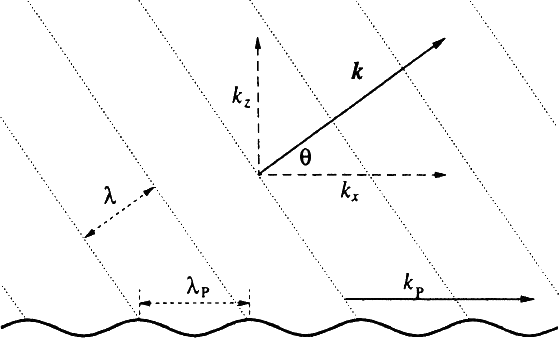
\includegraphics[width=0.7\linewidth]{00_Images/05_chapter/08.png}
    \caption{Wavevector matching and radiation angle for large vibrating plates}
    \label{fig:plate_radiation_angle}
\end{figure}

    %! TEX root = main.tex

\chapter{Pipes}

This chapter introduces wave propagation in ducts, with emphasis on cylindrical pipes as a model for wind instruments and for air cavities coupled to vibrating structures. The goal is to describe how the acoustic field evolves along the duct, how higher-order modes arise when the cross section cannot be treated as uniform, and how cutoff frequencies determine which modes can effectively propagate. 

\section{Infinite Cylindrical Pipes}

Let us consider an infinite cylindrical pipe deployed along the \( x \) axis, with cross section \( S \). Cylindrical coordinates \( (r,\phi,x) \) are used. We assume rigid, smooth, thermally insulating walls. The basic geometry and notation for an infinite cylindrical duct are summarized in figure \ref{fig:pipe_geometry}.

\begin{figure}[!htb]
    \centering
    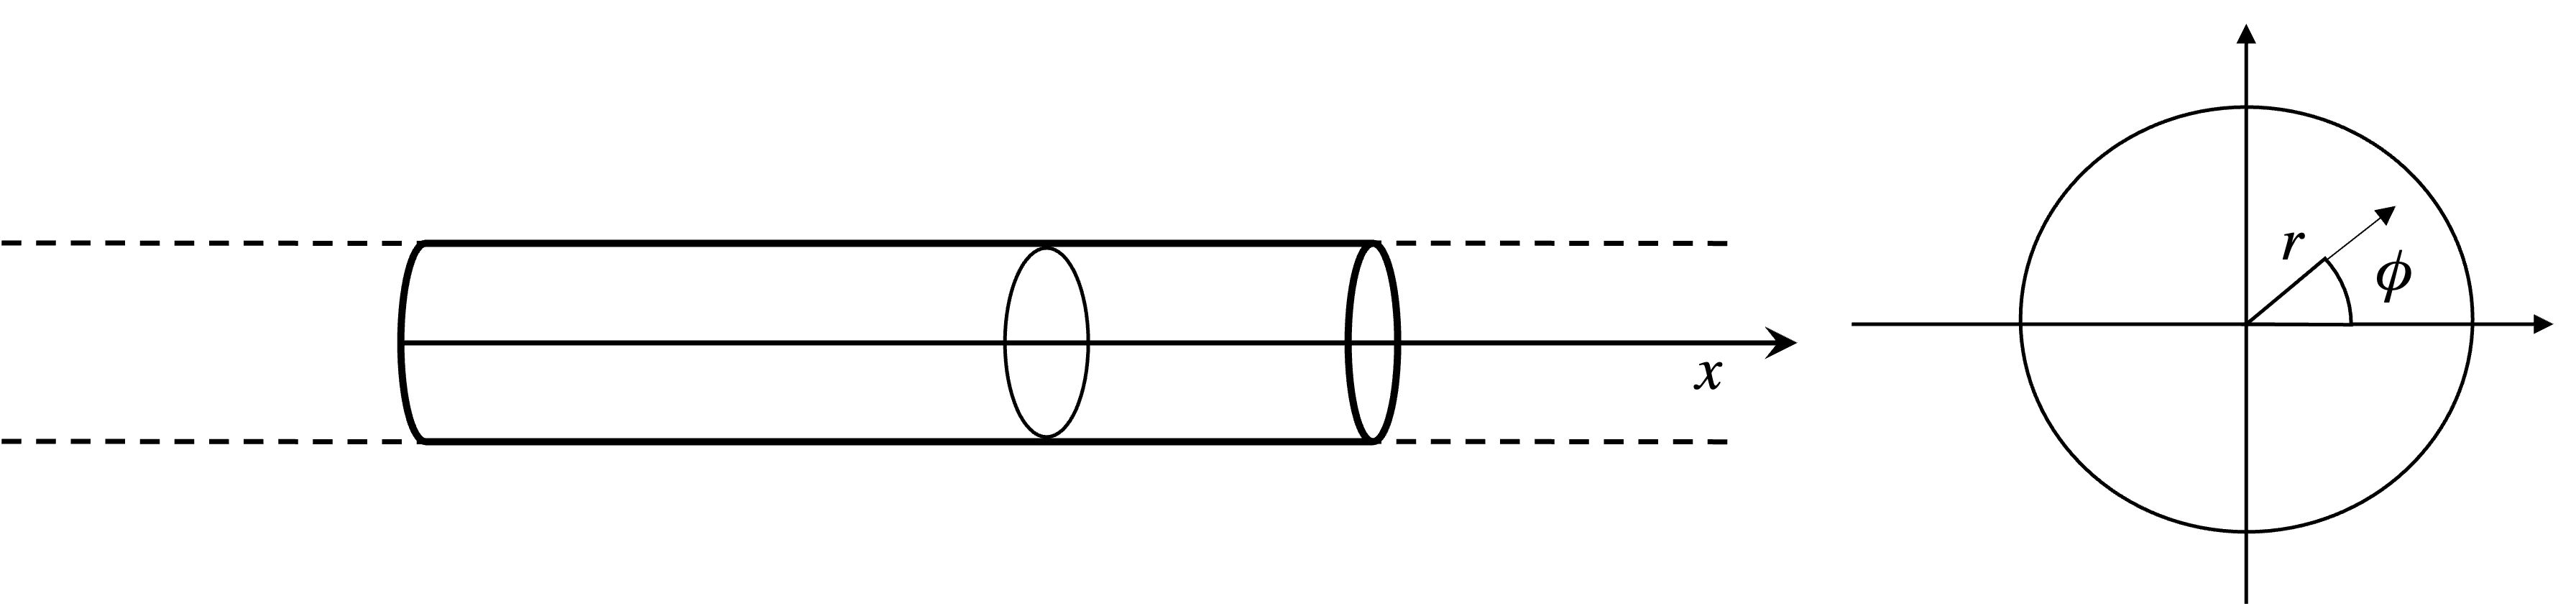
\includegraphics[width=0.60\linewidth]{00_Images/06_chapter/img66.jpg}
    \caption{Geometry of an infinite cylindrical pipe}
    \label{fig:pipe_geometry}
\end{figure}

\subsection{Plane-wave Approximation} 

If the pressure is assumed uniform over the cross section, it depends only on \( x \) and \( t \), and a traveling-wave solution can be written as
\[
p(x,t) = p e^{j(-kx+\omega t)}
\]
The acoustic volume flow is defined as \( U(x,t) \triangleq u(x,t)S \), and under this approximation it becomes
\[
U(x,t) = \frac{S p}{\rho c} e^{j(-kx+\omega t)}
\]
The corresponding characteristic impedance is
\[
Z_{0} = \frac{p(x,t)}{U(x,t)} = \frac{\rho c}{S}
\]
This quantity differs from the wave impedance because the denominator is the volume flow rather than the particle velocity.

\subsection{Wave Equation and Boundary Condition} 

In general, pressure and particle velocity are not uniform over the section, therefore \( p = p(r,\phi,x,t) \). The wave equation in cylindrical coordinates is
\[
\frac{1}{r}\frac{\partial}{\partial r}\left(r\frac{\partial p}{\partial r}\right) + \frac{1}{r^{2}}\frac{\partial^{2}p}{\partial \phi^{2}} + \frac{\partial^{2}p}{\partial x^{2}} = \frac{1}{c^{2}}\frac{\partial^{2}p}{\partial t^{2}}
\]
Let \( a \) be the pipe radius. Rigid walls imply that the radial component of particle velocity vanishes at \( r=a \),
\[
\left.u_{r}(r,\phi,x,t)\right|_{r=a} = 0
\]
Using the linear momentum equation
\[
\rho \frac{\partial \mathbf{u}}{\partial t} = -\nabla p
\]
this condition is equivalent to
\[
\left.\frac{\partial p}{\partial r}\right|_{r=a} = 0
\]

\subsection{Modal Solutions and Cutoff} 

\begin{figure}[!htb]
    \centering
    \subfloat[Pressure and transverse flow patterns]{%
        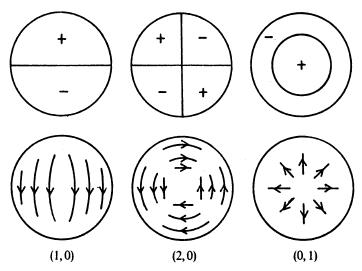
\includegraphics[width=0.4\linewidth]{00_Images/06_chapter/img92.jpg}%
    }\hfill
    \subfloat[Particle-velocity patterns (below cutoff)]{%
        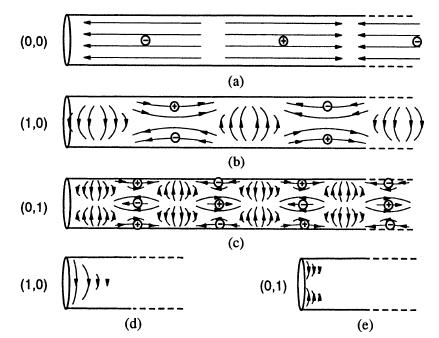
\includegraphics[width=0.4\linewidth]{00_Images/06_chapter/img107.jpg}%
    }
    \caption{Examples of higher-order modal field patterns in a cylindrical duct}
    \label{fig:higher_modes_patterns}
\end{figure}

After separation of variables, the \( (m,n) \) mode propagating in the tube can be written as
\[
p_{mn}(r,\phi,x,t) = p J_{m}\left(\frac{\pi q_{mn} r}{a}\right)
\begin{cases}
\cos(m\phi) \\
\sin(m\phi)
\end{cases}
e^{-jk_{mn}x}e^{j\omega t}
\]
where \( J_{m} \) is the Bessel function of order \( m \). The boundary condition \( \partial p/\partial r|_{r=a}=0 \) requires
\[
J_{m}'(\pi q_{mn}) = 0
\]
therefore \( \pi q_{mn} \) must coincide with a zero of \( J_{m}' \). The axial wavenumber satisfies
\[
k_{mn}^{2} = \left(\frac{\omega}{c}\right)^{2} - \left(\frac{\pi q_{mn}}{a}\right)^{2}
\]
A mode propagates without radial attenuation only if \( k_{mn} \) is real, which defines the cutoff frequency
\[
\omega_{c} = \frac{\pi q_{mn} c}{a}
\]
Below cutoff, the mode becomes evanescent and is strongly attenuated along the duct. The only exception is the \( (0,0) \) mode, for which \( q_{00}=0 \), corresponding to the plane wave that propagates at all frequencies. The index \( m = 0,1,2,\dots \) represents the number of nodal diameters, while \( n = 0,1,2,\dots \) represents the number of nodal circles in the cross section. The transverse structure of higher-order duct modes is illustrated in figure \ref{fig:higher_modes_patterns}.

\section{Wall Losses}

In the ideal plane-wave approximation for the \( (0,0) \) mode, both the axial particle velocity \( u_{x} \) and the pressure \( p \) are assumed uniform over the pipe cross section. In practice, measurements show that they are maximum along the pipe axis and decrease towards the walls. This deviation is due to wall losses, mainly caused by viscous drag and thermal exchange with the pipe boundaries.

\subsection{Viscous Losses} 

Viscous drag exerted by the walls reduces the particle velocity close to the boundary. Wall losses can be interpreted through the development of a viscous boundary layer near the duct wall, as shown in figure \ref{fig:boundary_layer}.

\begin{figure}[!htb]
    \centering
    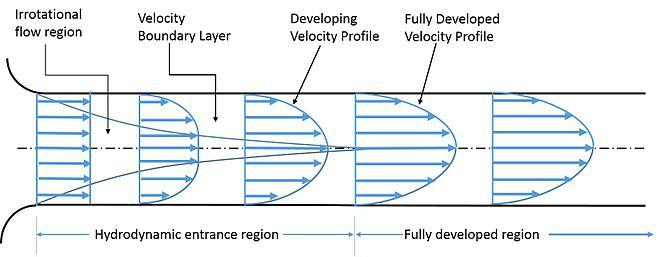
\includegraphics[width=0.75\linewidth]{00_Images/06_chapter/img117.jpg}
    \caption{Development of the viscous boundary layer in the plane-wave mode}
    \label{fig:boundary_layer}
\end{figure}

The region over which this effect is significant is referred to as the viscous boundary layer. Its relevance can be quantified by comparing its thickness to the pipe radius through the dimensionless ratio \( r_{v} \). A commonly used expression is
\[
r_{v} = 632.8 a f^{1/2}(1 - 0.0029\Delta T)
\]
where \( a \) is the pipe radius, \( f \) is the frequency, and \( \Delta T = T - \SI{300}{\kelvin} \). Viscous losses are therefore more important for small pipes.

\subsection{Thermal Losses} 
A similar mechanism arises from heat exchange between air and the walls. The resulting thermal boundary layer modifies the effective compressibility of the air close to the boundary. The associated ratio is
\[
r_{t} = 532.8 a f^{1/2}(1 - 0.0031\Delta T)
\]
with the same definitions as above. 

\subsection{Consequences on Propagation} 

The combined effect of viscous and thermal losses makes the characteristic impedance \( Z_{0} \) complex and different from \( \rho c/S \), and the wavenumber becomes complex as well, leading to attenuation along the duct. Writing
\[
k = \frac{\omega}{v} - j\alpha
\]
the phase velocity \( v \) and the attenuation coefficient \( \alpha \) can be described as functions of \( r_{v} \). For sufficiently large tubes, approximate expressions valid for \( r_{v} > 10 \) are
\[
v \approx c\left[1 - \frac{1.65 \times 10^{-3}}{a f^{1/2}}\right]
\]
\[
\alpha \approx \frac{3 \times 10^{-5} f^{1/2}}{a}
\]
The trends are summarized in the plots of the real and imaginary parts of \( Z_{0} \) as functions of \( r_{v} \), and of \( v/c \) and \( \alpha/f \) versus \( r_{v} \). The influence of viscous and thermal losses on the characteristic impedance is summarized in figure \ref{fig:char_impedance_parts} and the corresponding effects on phase speed and attenuation are illustrated in figure \ref{fig:phase_speed_attenuation}.

\begin{figure}[!htb]
    \centering
    \subfloat{%
        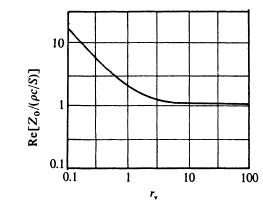
\includegraphics[width=0.4\linewidth]{00_Images/06_chapter/img148.jpg}%
    }\hfill
    \subfloat{%
        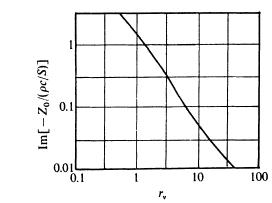
\includegraphics[width=0.4\linewidth]{00_Images/06_chapter/img158.jpg}%
    }
    \caption{Real and imaginary parts of the characteristic impedance versus the loss parameter}
    \label{fig:char_impedance_parts}
\end{figure} 

\begin{figure}[!htb]
    \centering
    \subfloat{%
        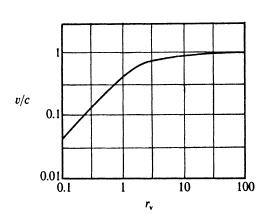
\includegraphics[width=0.4\linewidth]{00_Images/06_chapter/img206.jpg}%
    }\hfill
    \subfloat{%
        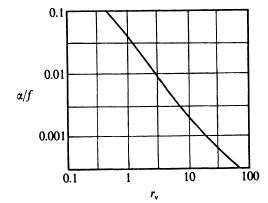
\includegraphics[width=0.4\linewidth]{00_Images/06_chapter/img216.jpg}%
    }
    \caption{Phase speed and attenuation coefficient in a lossy cylindrical duct}
    \label{fig:phase_speed_attenuation}
\end{figure}

\section{Finite Cylindrical Pipes}

From now on we assume that only the plane mode \( m = 0 \), \( n = 0 \) is present, so that pressure and volume flow depend on \( x \) and \( t \) only. The pressure field is written as the superposition of two counter-propagating waves
\[
p(x,t) = \left[Ae^{-jkx} + Be^{jkx}\right]e^{j\omega t}
\]
Using \( \rho \partial u/\partial t = -\nabla p \), the acoustic volume flow \( U(x,t) = Su(x,t) \) becomes
\[
U(x,t) = \frac{S}{\rho c}\left[Ae^{-jkx} - Be^{jkx}\right]e^{j\omega t}
\]
where \( S \) is the cross-sectional area and \( Z_{0} = \rho c/S \) is the characteristic impedance of the duct.

\subsection{Termination and Input Impedance}

Let the duct be terminated at \( x=L \) by a load impedance \( Z_{L} \), defined by
\[
\frac{p(L,t)}{U(L,t)} = Z_{L}
\]
Imposing the termination condition yields ratio between backward and forward waves
\[
\frac{B}{A} = e^{-2jkL}\left(\frac{Z_{L} - Z_{0}}{Z_{L} + Z_{0}}\right)
\]
The input impedance, defined at \( x=0 \) as \( Z_{\mathrm{IN}} = p(0,t)/U(0,t) \), is
\[
Z_{\mathrm{IN}} = Z_{0}\left[\frac{Z_{L}\cos(kL) + jZ_{0}\sin(kL)}{jZ_{L}\sin(kL) + Z_{0}\cos(kL)}\right]
\]

\begin{figure}[!htb]
    \centering
    \subfloat[Stopped End]{%
        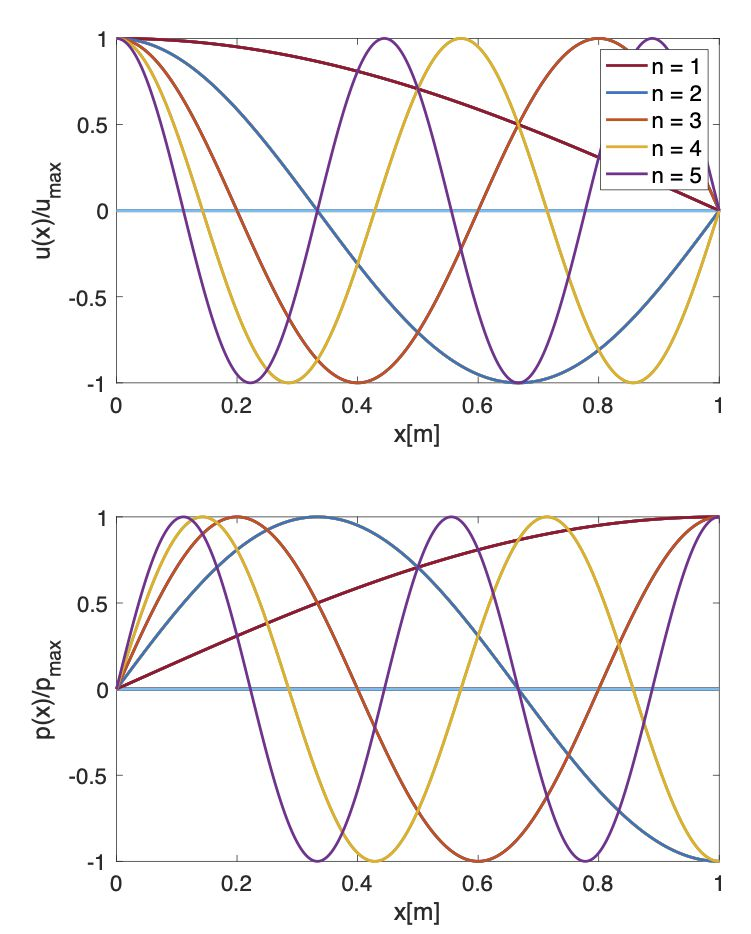
\includegraphics[height=0.4\textheight]{00_Images/06_chapter/img230.jpg}%
    }\hfill
    \subfloat[Open End]{%
        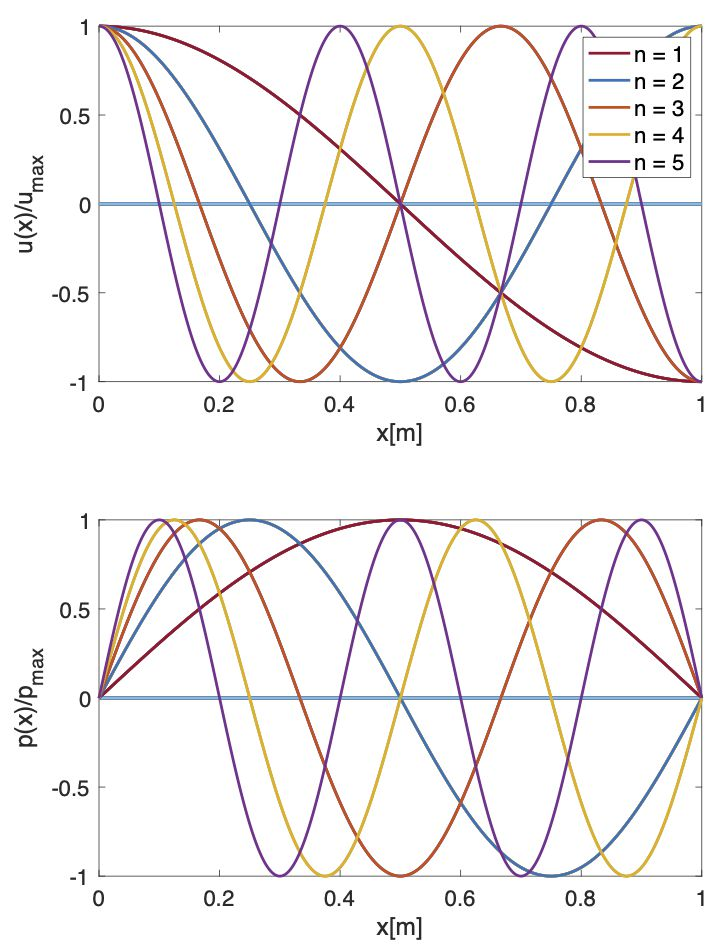
\includegraphics[height=0.4\textheight]{00_Images/06_chapter/img241.jpg}%
    }
    \caption{Examples of pressure and velocity distributions in finite pipes}
    \label{fig:finite_pipe_fields}
\end{figure}

\subsection{Stopped End}

For a stopped termination \( Z_{L} \to \infty \), the input impedance reduces to
\[
Z_{\mathrm{IN}}^{\mathrm{stopped}} = -jZ_{0}\cot(kL)
\]
Impedance minima occur at
\[
\omega_{\mathrm{stopped}} = \frac{(2n-1)\pi c}{2L}
\]
which corresponds to an odd number of quarter wavelengths in the pipe. 

\subsection{Open End and Radiation Load}

For an ideal open termination \( Z_{L} = 0 \),
\[
Z_{\mathrm{IN}}^{\mathrm{open}} = jZ_{0}\tan(kL)
\]
and for \( kL \ll 1 \),
\[
Z_{\mathrm{IN}}^{\mathrm{open}} \approx jZ_{0}kL
\]
The corresponding impedance minima occur at
\[
\omega_{\mathrm{open}} = \frac{n\pi c}{L}
\]
which corresponds to an even number of quarter wavelengths. In practice, a truly open end implies radiation outside the duct, therefore the termination cannot be modeled with \( p(L,t)=0 \) and a radiation load must be introduced.

\subsection{End Correction}

If the pipe terminates in a plane flange, the radiation load can be written as \( Z_{\mathrm{flanged}} = R + jX \) with
\[
R = Z_{0}\left[\frac{(ka)^{2}}{2} - \frac{(ka)^{4}}{2^{2}\cdot 3} + \frac{(ka)^{6}}{2^{2}\cdot 3^{2}\cdot 4} - \dots\right]
\]
\[
X = \frac{Z_{0}}{\pi k^{2}a^{2}}\left[\frac{(2ka)^{3}}{3} - \frac{(2ka)^{5}}{3^{2}\cdot 5} + \frac{(2ka)^{7}}{3^{2}\cdot 5^{2}\cdot 7} - \dots\right]
\]
In the region \( ka \ll 1 \), the impedance is approximately reactive
\[
Z_{\mathrm{flanged}} \approx jZ_{0}k\left(\frac{8a}{3\pi}\right)
\]
Since a short open pipe segment of length \( \Delta \) has \( Z_{\mathrm{IN}} \approx jZ_{0}k\Delta \) for \( k\Delta \ll 1 \), the radiation load can be assimilated to a virtual elongation
\[
\Delta_{\mathrm{flanged}} = \frac{8a}{3\pi} \approx 0.85a
\]
Therefore a real open pipe can be approximated as an ideal open pipe of effective length \( L + \Delta_{\mathrm{flanged}} \), so that radiation is included through an end correction. For an unflanged pipe, a commonly used low-frequency approximation is
\[
\Delta_{\mathrm{unflanged}} \approx 0.6a
\]
The end-correction model can be extended with reasonable accuracy up to \( ka = 3 \). For \( ka > 3 \), radiation losses become significant and the load cannot be treated as purely reactive, so the simple virtual-elongation picture is no longer sufficient. The frequency dependence of the end correction is shown in figure \ref{fig:end_correction}.

\begin{figure}[!htb]
    \centering
    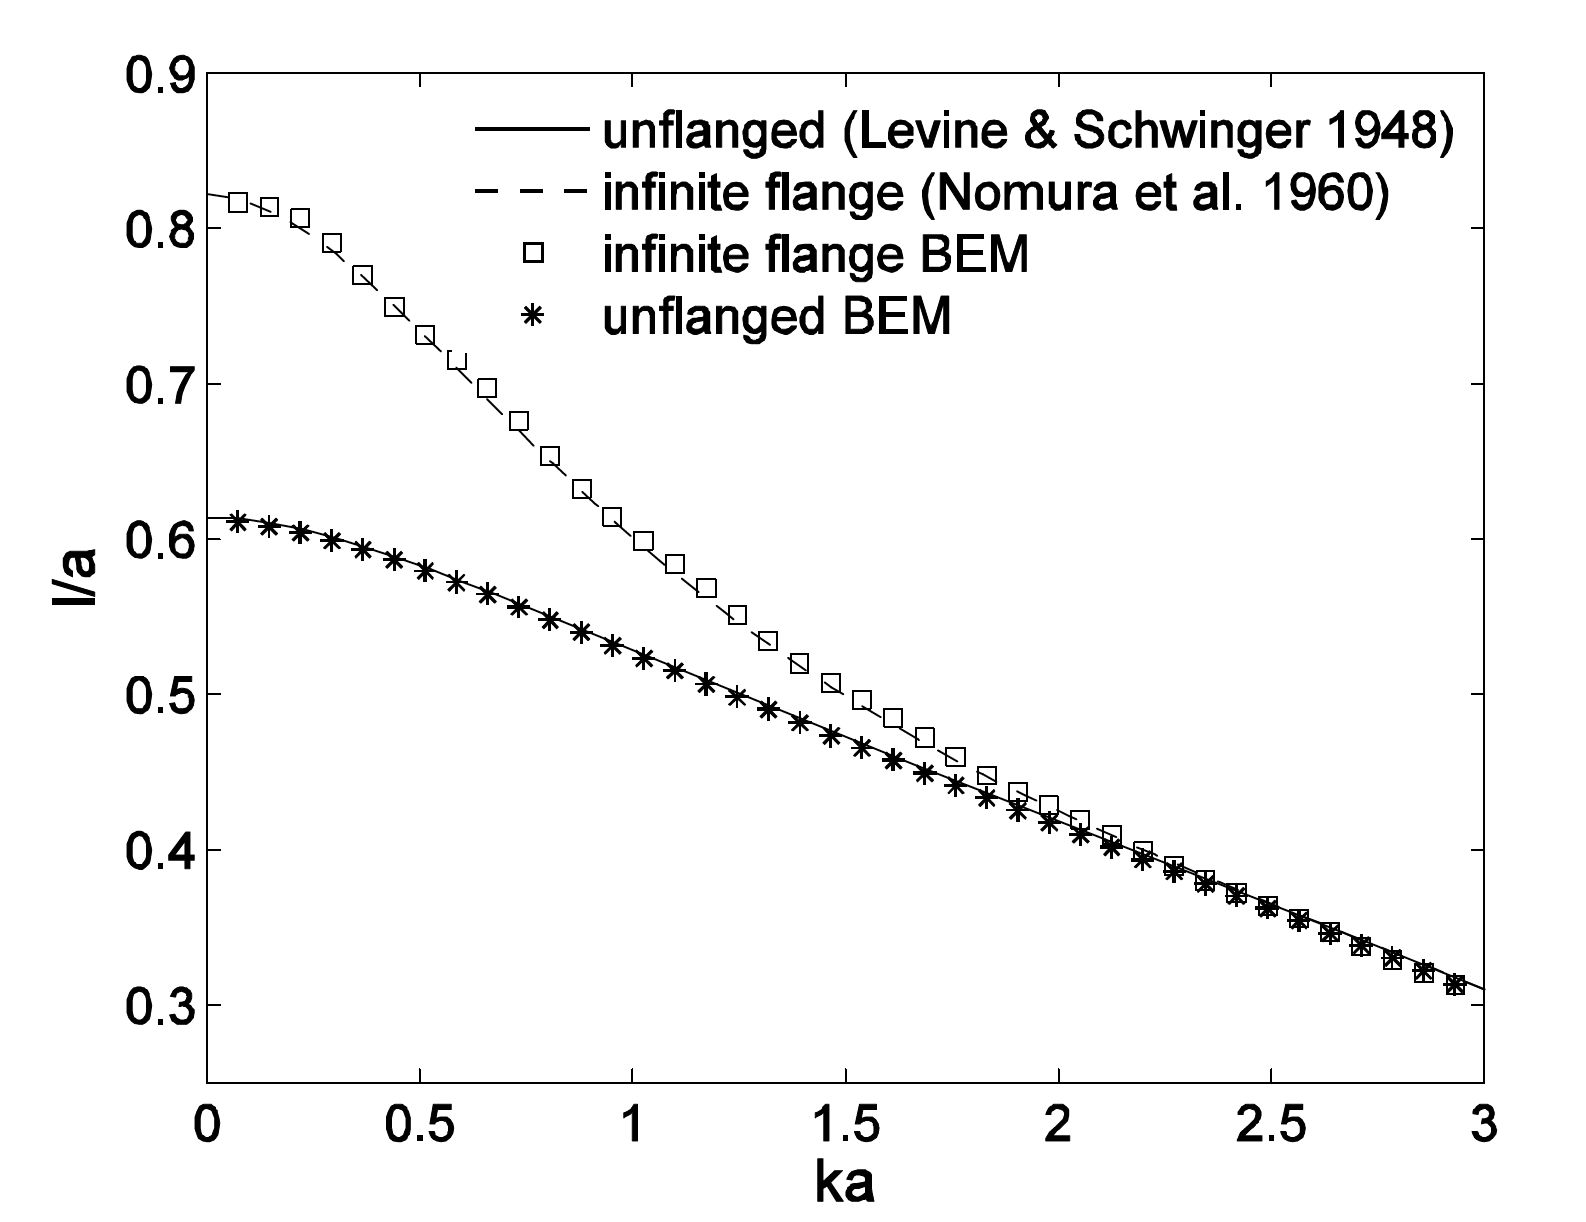
\includegraphics[width=0.80\linewidth]{00_Images/06_chapter/img265.jpg}
    \caption{Normalized end correction for flanged and unflanged terminations}
    \label{fig:end_correction}
\end{figure}


\subsection{Directional Properties and Directivity Index}

The directional properties of the radiation can be described through the angular distribution of intensity. The radiated intensity at angle \( \theta \) is proportional to
\[
\left[\frac{2J_{1}(ka\sin\theta)}{ka\sin\theta}\right]^{2}
\]
where \( J_{1} \) is the Bessel function of first order. A compact summary of directionality is provided by the directivity index \( DI \), defined as the sound intensity on the axis compared with that of an isotropic source radiating the same total radiated power. The transition from nearly omnidirectional radiation to more directional patterns with increasing \( ka \) is illustrated in figure \ref{fig:pipe_directivity}.

\begin{figure}[!htb]
    \centering
    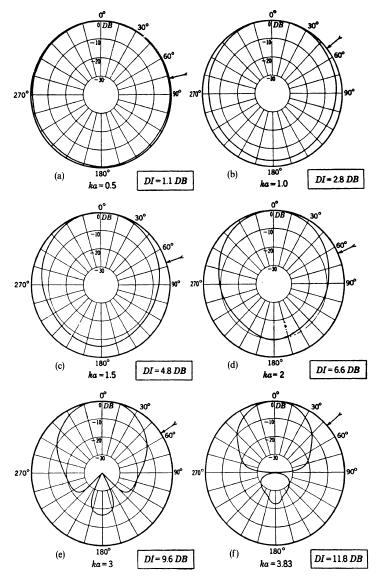
\includegraphics[width=0.60\linewidth]{00_Images/06_chapter/img282.jpg}
    \caption{Radiation directivity of a circular pipe opening for increasing \(ka\)}
    \label{fig:pipe_directivity}
\end{figure}

\section{Impedance Curves}

Including wall losses leads to a complex wavenumber
\[
k = \frac{\omega}{v} - j\alpha
\]
where \( v \) is the phase velocity and \( \alpha \) is the attenuation coefficient. As a consequence, the input impedance of a finite pipe can be expressed in terms of hyperbolic functions. For an open pipe, a convenient form is
\[
Z_{\mathrm{IN}} = Z_{0}\left[\frac{\tanh(\alpha L) + j\tan(\omega L/v)}{1 + j\tanh(\alpha L)\tan(\omega L/v)}\right]
\]
The auxiliary functions \( \tanh(\cdot) \) and \( \coth(\cdot) \) are often used to describe how the resonance peaks are affected by losses. 

\subsection{Maxima and Minima}

Wall losses do not modify the location of maxima and minima with respect to the ideal lossless case, but they strongly affect their magnitude. In particular, the impedance magnitude at resonance maxima is
\[
|Z_{\mathrm{IN}}|_{\max} = Z_{0}\coth(\alpha L)
\]
while at the minima it is
\[
|Z_{\mathrm{IN}}|_{\min} = Z_{0}\tanh(\alpha L)
\]
Since \( \alpha \) increases with frequency, the maxima of \( Z_{\mathrm{IN}} \) progressively converge to \( Z_{0} \) at high frequencies.

\subsection{Role of Pipe Size}

The relative importance of the different loss mechanisms depends on the pipe radius. In narrow pipes, wall losses dominate already at low frequencies. In wide pipes, wall losses are weaker and radiation losses from the open end become more important at high frequencies. This behavior is reflected by the impedance curves shown for a pipe of length \SI{1}{\metre} with radius \SI{2}{\centi\metre} and \SI{10}{\centi\metre}, where the peak magnitudes evolve differently with frequency. The effect of duct radius on the input impedance in the presence of losses is illustrated in figure \ref{fig:wide_narrow_impedance}.

\begin{figure}[!htb]
    \centering
    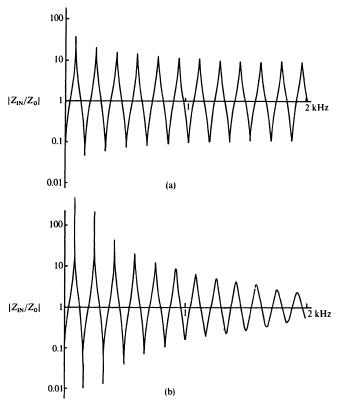
\includegraphics[width=0.60\linewidth]{00_Images/06_chapter/img327.jpg}
    \caption{Input impedance comparison for wide and narrow cylindrical pipes}
    \label{fig:wide_narrow_impedance}
\end{figure}

\section{Horns}

In horns the cross section varies along the axis, therefore the planar-wave assumption becomes less accurate. A useful approximation can be obtained when the horn does not flare too rapidly. In this case, wavefronts can be treated as spherical and orthogonal to the horn walls. The wavefront can be represented as a spherical cap of area \( S \) with curvature radius \( r \), and an equivalent circular cross section of radius \( a \). The geometrical interpretation is summarized in figure \ref{fig:webster_geometry}.

\begin{figure}[!htb]
    \centering
    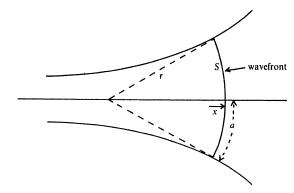
\includegraphics[width=0.45\linewidth]{00_Images/06_chapter/img343.jpg}
    \caption{Wavefront geometry and cross-sectional area \(S(x)\) in a horn}
    \label{fig:webster_geometry}
\end{figure}

\subsection{Horn Wave Equation and Propagation Condition}

Let \( x \) be the coordinate along the horn axis. Due to the progressive increase of the cross section, the pressure amplitude decreases with \( x \). It is convenient to introduce
\[
\psi = p S^{-1/2}
\]
For a circular horn, \( \psi \) satisfies
\[
\frac{\partial^{2}\psi}{\partial x^{2}} + \left(k^{2} - \frac{1}{a}\frac{\partial^{2}a}{\partial x^{2}}\right)\psi = 0
\]
with \( k = \omega/c \). The quantity
\[
F = \frac{1}{a}\frac{\partial^{2}a}{\partial x^{2}}
\]
is the barrier function of the horn. The solution corresponds to a propagating wave if
\[
k^{2} - F > 0
\]
therefore frequencies such that \( k^{2} > F \) can propagate, whereas frequencies such that \( k^{2} < F \) do not propagate.

\subsection{Slowly Flaring Horns}

For horns that do not flare too rapidly, \( F \) can be approximated as
\[
F \approx \frac{1}{R_{L}R_{T}}
\]
where \( R_{L} \) is the longitudinal radius of curvature and \( R_{T} \) is the internal transverse radius of curvature. This two radii of curvature are defined in figure \ref{fig:curvature_radii}.

\begin{figure}[!htb]
    \centering
    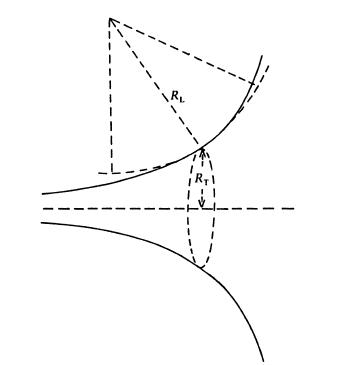
\includegraphics[width=0.45\linewidth]{00_Images/06_chapter/img359.jpg}
    \caption{Definition of longitudinal and transverse curvature radii \(R_L\) and \(R_T\)}
    \label{fig:curvature_radii}
\end{figure}

\subsection{Salmon Horns}

In Salmon horns the barrier function \( F \) is constant along the axis, hence the cutoff frequency is constant throughout the horn. An equivalent radius can be written as
\[
a = a_{0}\left[\cosh(mx) + T\sinh(mx)\right]
\]
A corresponding pressure wave is
\[
p = \left(\frac{p_{0}}{a}\right)e^{j\omega t}e^{-j\sqrt{k^{2}-m^{2}}x}
\]
and it does not propagate if \( k < m \). Different horn profiles are obtained by varying \( T \). 

\paragraph{Exponential horn} If \( T = 1 \),
\[
a = a_{0}e^{mx}
\]

\paragraph{Catenoidal horn} If \( T = 0 \),
\[
a = a_{0}\cosh(mx)
\]
This profile smoothly joins a cylindrical pipe extending along the negative axis to the origin.

\paragraph{Conical horn} If \( T = 1/(mx_{0}) \) and \( m \to 0 \),
\[
a = a_{0}\left(1 + \frac{x}{x_{0}}\right)
\]
The vertex is at \( -x_{0} \) and the semiangle is \( \tan^{-1}(a_{0}/x_{0}) \). In this case \( F = 0 \), therefore the conical horn has no cutoff.

\section{Finite Conical and Bessel Horns}

In practical instruments horns have finite length and are connected to the rest of the duct by a throat section. The input impedance must therefore account for the termination at the mouth and for the geometric parameters of the profile. 

\subsection{Finite Conical and Exponential Horns}

Consider a conical horn with throat area \( S_{1} \) at position \( x_{1} \) and mouth area \( S_{2} \) at position \( x_{2} \), with \( L = x_{2} - x_{1} \). If the horn is terminated by a load impedance \( Z_{L} \) at the mouth, the input impedance at the throat can be written as
\[
Z_{\mathrm{IN}} = \frac{\rho c}{S_{1}}
\frac{
jZ_{L}\left[\sin(kL-\theta_{2})/\sin\theta_{2}\right] + (\rho c/S_{2})\sin kL
}{
Z_{L}\left[\sin(kL+\theta_{1}-\theta_{2})/(\sin\theta_{1}\sin\theta_{2})\right] - (j\rho c/S_{2})\left[\sin(kL+\theta_{1})/\sin\theta_{1}\right]
}
\]
where the angles \( \theta_{1} \) and \( \theta_{2} \) depend on the distance from the cone apex. In particular, defining \( x_{1/2} \) as the distance from the apex,
\[
\theta_{1}/2 = \tan^{-1}(kx_{1/2})
\]
For an exponential horn of length \( L \), the input impedance can be expressed as
\[
Z_{\mathrm{IN}} = \frac{\rho c}{S_{1}}
\frac{
Z_{L}\cos(bL+\theta) + j(\rho c/S_{2})\sin bL
}{
jZ_{L}\sin bL + (\rho c/S_{2})\cos(bL-\theta)
}
\]
with
\[
b^{2} = k^{2} - m^{2}
\]
and
\[
\theta = \tan^{-1}(m/b)
\]
A representative magnitude of the input impedance for a conical horn is shown in figure \ref{fig:conical_horn_impedance}.

\begin{figure}[!htb]
    \centering
    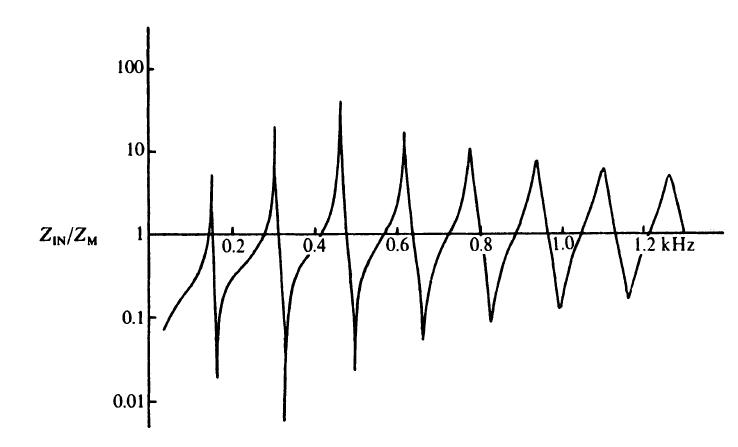
\includegraphics[width=0.7\linewidth]{00_Images/06_chapter/img375.jpg}
    \caption{Magnitude of the input impedance of a conical horn}
    \label{fig:conical_horn_impedance}
\end{figure}

\subsection{Conical Horns}

For an open conical horn, \( Z_{L} = 0 \), and the previous expression reduces to
\[
Z_{\mathrm{IN}} = j\left(\frac{\rho c}{S_{1}}\right)\frac{\sin kL \sin\theta_{1}}{\sin(kL+\theta_{1})}
\]
Zeros occur when \( \sin kL = 0 \), hence at the same frequencies as an open cylindrical pipe of length \( L \). Maxima occur when the denominator vanishes, which can be written as
\[
kL = n\pi - \tan^{-1}(kx_{1})
\]
The impedance magnitude therefore exhibits a sequence of peaks whose spacing remains essentially harmonic, while their heights decrease as frequency increases, consistently with the trend shown by the normalized impedance plot for a \SI{1}{\metre} horn. 

\subsection{Bessel Horns and Rapidly Flaring Profiles}

A broader class of horn profiles is described by Bessel horns, defined by
\[
S = Bx^{-2\epsilon}
\]
and
\[
a = bx^{-\epsilon}
\]
where \( x \) is the distance from a reference point \( x=0 \). When \( \epsilon > 0 \), the horn flares rapidly. For rapidly flaring horns it is important to interpret the barrier function with care. For exponential horns, a plane-wave based description predicts that the barrier function becomes unbounded as \( x \to 0 \), which would imply no propagation in that region. An example of Bessel-horn profile is shown in figure \ref{fig:bessel_horn_shape}. However, the plane-wave approximation is not applicable when the flare is rapid. Close to the open end, a spherical-wave description is more appropriate and leads to a different effective barrier function, as illustrated by the comparison between plane-wave and spherical-wave horn functions. The horn function and the accuracy of common approximations are compared in figure \ref{fig:horn_function_F}.

\begin{figure}[!htb]
    \centering
    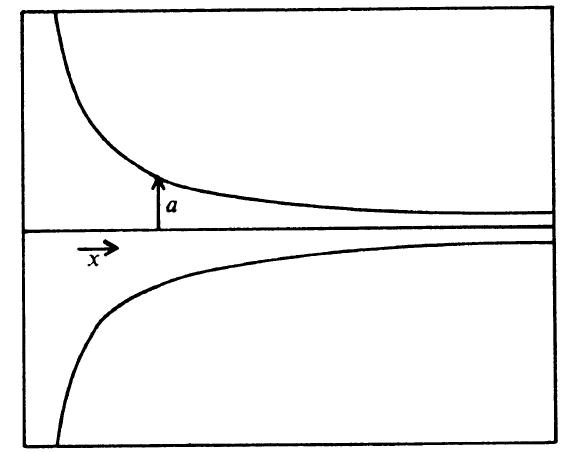
\includegraphics[width=0.50\linewidth]{00_Images/06_chapter/img391.jpg}
    \caption{Example geometry of a Bessel horn}
    \label{fig:bessel_horn_shape}
\end{figure}

\begin{figure}[!htb]
    \centering
    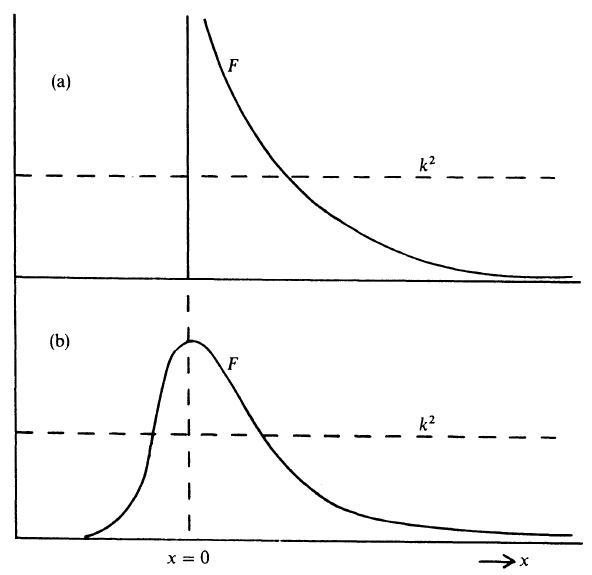
\includegraphics[width=0.60\linewidth]{00_Images/06_chapter/img407.jpg}
    \caption{Horn function \(F\) for Bessel cones: plane-wave and spherical-wave approximations}
    \label{fig:horn_function_F}
\end{figure}

\section{Compound Horns}

Most brass instruments are based on the combination of different duct profiles, rather than on a single uniform geometry. A typical configuration consists of a section with constant cross section followed by an expanding section. Two common examples are a conical horn smoothly joined to a cylindrical section, which is representative of older instruments, and a conical horn smoothly joined to an exponential section, which is representative of modern designs. 

\subsection{Cylindrical Throat Coupled to a Conical Mouth}

Let us consider a cylindrical section of length \( L_{2} \) connected to a conical section of length \( L_{1} \). The overall input impedance is obtained by using, as terminating impedance of the cylindrical section, the input impedance of the conical one. The input impedance of the conical section, evaluated at the junction with area \( S_{1} \), is
\[
Z_{c} = \frac{j\rho c}{S_{1}}\left(\cot kL_{1} + \frac{1}{kx_{1}}\right)^{-1}
\]
where \( x_{1} \) is the distance from the cone apex to the junction. This impedance plays the role of load \( Z_{L} \) for the cylindrical throat. Replacing \( Z_{L} = Z_{c} \) into the expression of the input impedance of the cylindrical section yields a condition for the maxima of the global input impedance. These maxima are found where
\[
\tan kL_{2} - \cot kL_{1} - \left(\frac{1}{kx_{1}}\right) = 0
\]
The resulting peak pattern depends on the relative lengths \( L_{1} \) and \( L_{2} \), as illustrated by the impedance-maxima plot for the compound geometry. The relation between horn shape and the positions of impedance maxima is illustrated in figure \ref{fig:compound_horn_maxima}.

\begin{figure}[!htb]
    \centering
    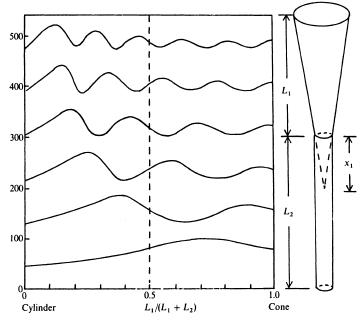
\includegraphics[width=0.55\linewidth]{00_Images/06_chapter/img423.jpg}
    \caption{Maxima of input impedance for a compound horn profile}
    \label{fig:compound_horn_maxima}
\end{figure}

\subsection{Cylindrical Throat Coupled to an Exponential Mouth}

A similar procedure applies when the cylindrical section is connected to an exponential horn. In that case, the condition for the maxima of the global input impedance can be written as
\[
\tan kL_{2} - \frac{b}{k}\cot bL_{1} - \frac{m}{k} = 0
\]
where
\[
b = (k^{2} - m^{2})^{1/2}
\]
and \( m \) is the exponential flare parameter. 

\section{Perturbations}

In real wind instruments the duct geometry is rarely smooth and uniform. Local irregularities, such as fingerholes or small changes in cross section, introduce perturbations that modify the resonance frequencies. These effects can be exploited to tune the instrument response and to obtain a desired harmonic structure. Let the nominal section be \( S_{0}(x) \) and introduce a small perturbation \( \delta S(x) \), so that
\[
S(x) = S_{0}(x) + \delta S(x)
\]
The corresponding pressure distribution is written as
\[
p(x,t) = \beta p_{0}(x,t) + p_{1}(x,t)
\]
where \( p_{0} \) is the unperturbed solution and \( \beta \approx 1 \) under the assumption of a small perturbation. The perturbed resonance frequency is
\[
\omega = \omega_{0} + \delta\omega
\]
By substituting these expressions into the wave equation, retaining first-order terms, and integrating over the horn length, the resonance shift can be written as
\[
\delta\omega
=
-\frac{c^{2}}{2\omega_{0}N}
\int S_{0}\frac{d}{dx}\left(\frac{\delta S}{S_{0}}p_{0}\frac{dp_{0}}{dx}\right)dx
\]
where
\[
N = \int S_{0}p_{0}^{2}dx
\]

\subsection{Localized Perturbation}

Consider a localized change of section modeled as
\[
\delta S(x) = \Delta\delta(x-x_{0})
\]
After integration one obtains 
\[
\delta\omega
=
\frac{c^{2}\Delta}{2\omega_{0}N}
\left[
\frac{d}{dx}\left(p_{0}\frac{dp_{0}}{dx}\right)
\right]_{x=x_{0}}
\]
If the unperturbed mode shape is \( p_{0}(x,t) = \sin(kx)\sin(\omega t) \), then
\[
\delta\omega \propto \cos(2kx_{0})
\]
Therefore, if the enlargement is located close to a pressure maximum, \( \cos(2kx_{0})=-1 \) and the resonance frequency is lowered. If it is located close to a pressure minimum, \( \cos(2kx_{0})=+1 \) and the resonance frequency is increased. For a local reduction of the cross section the opposite trends apply. 

\section{Curved Horns}

Bending is often introduced in wind instruments to keep the overall extension within a reasonable size while preserving the acoustic length. Curvature modifies the propagation conditions inside the duct, leading to changes in phase velocity and characteristic impedance. The curvature can be described through the dimensionless parameter
\[
B = \frac{r}{R}
\]
where \( r \) is the radius of the circular cross section and \( R \) is the curvature radius. The influence of curvature on wave speed and characteristic impedance is summarized in figure \ref{fig:curved_horn_effects}.

\begin{figure}[!htb]
    \centering
    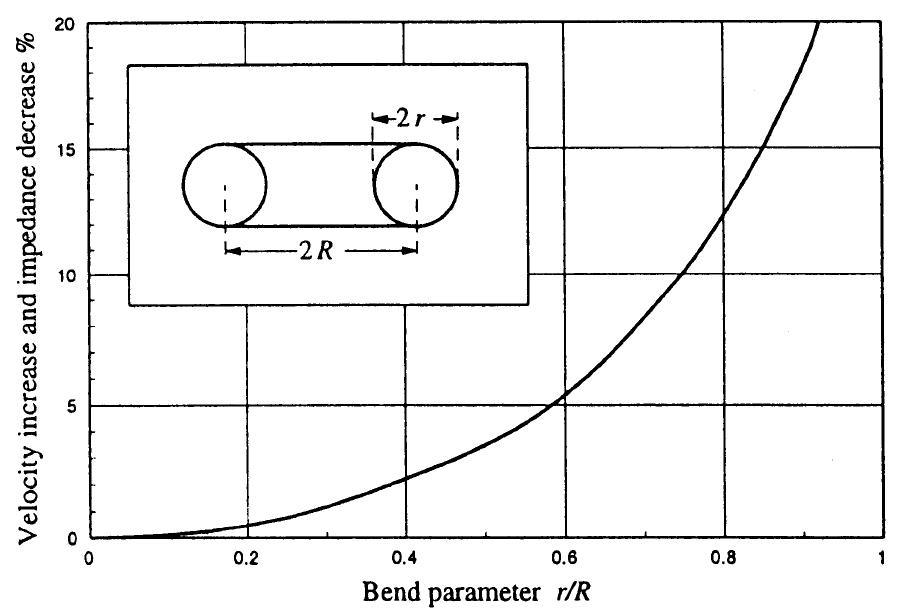
\includegraphics[width=0.7\linewidth]{00_Images/06_chapter/img445.jpg}
    \caption{Effect of horn curvature on wave speed and impedance versus \( B = r/R \)}
    \label{fig:curved_horn_effects}
\end{figure}

For a curved horn, the relative increase in phase velocity and the relative decrease in duct impedance can be expressed as
\[
\frac{\delta v}{c} = -\frac{\delta Z}{Z_{0}} = \left(\frac{2I}{\pi B}\right)^{1/2} - 1
\]
with
\[
I = \int_{0}^{\pi/2} \cos\theta \ln\left(\frac{1 + B\cos\theta}{1 - B\cos\theta}\right)d\theta
\]
As shown by the plot of \( \delta v \) and \( -\delta Z \) versus \( B \), the effect is negligible for small curvature but grows rapidly as \( B \) increases.

\section{Analysis in the Time Domain}

The analysis in the time domain is useful to describe the transient behavior of a wind instrument. Starting from the input impedance \( Z(\omega) \), its inverse Fourier transform defines the Green function \( G(t) \), which relates the acoustic volume flow \( U(t) \) to the pressure \( p(t) \) through convolution
\[
p(t) = \int_{-\infty}^{t} G(t-t')U(t')dt' = G(t)\star U(t)
\]
A direct evaluation is often inconvenient because \( G(t) \) may have a large time support. 

\subsection{Reflection Function Formulation}

Define the plane-wave reflection function at the instrument input as
\[
r(\omega) = \frac{Z(\omega)-Z_{0}}{Z(\omega)+Z_{0}}
\]
where \( Z_{0} \) is the characteristic impedance of the cylindrical reference duct. This implies
\[
Z(\omega) = Z_{0} + Z_{0}r(\omega) + r(\omega)Z(\omega)
\]
Taking the inverse Fourier transform yields
\[
G(t) = Z_{0}\delta(t) + Z_{0}\delta(t)\star r(t) + r(t)\star G(t)
\]
and substituting into the pressure relation gives
\[
p(t) = Z_{0}U(t) + Z_{0}r(t)\star U(t) + r(t)\star p(t)
\]
Equivalently,
\[
p(t) = Z_{0}U(t) + \int_{0}^{\infty} r(t')\left[Z_{0}U(t-t') + p(t-t')\right]dt'
\]

\subsection{Practical Approximation}

The pressure \( p(t) \) is zero for times shorter than the wave-return transit time \( \tau \) along the cylindrical part of the bore. Moreover, \( p(t) \) is smaller than \( G(t) \) because the returning waves are partially absorbed by the matching input termination. These observations justify neglecting the term involving \( p(t-t') \) inside the integral, which makes the computation feasible in practice. 

\section{Coupling Between Pipe and Mechanical Oscillator}

The goal of this section is to illustrate how the coupling between an air cavity and an elastic structure modifies the dynamics of the structure. This situation is encountered in most stringed instruments and also in many percussion instruments. The structure is modeled as a single-degree-of-freedom oscillator, while the cavity is assumed one-dimensional. 

\subsection{Governing Equations}

We consider a pipe of cross section \( S \) and length \( L \), excited at \( x=0 \) by a mechanical oscillator of mass \( M \), resonance angular frequency \( \omega_{0} \), and reduced damping \( \zeta_{0} \). The excitation force is \( f(t) \). Visco-thermal losses in the pipe are neglected. The pipe is terminated at \( x=L \) by a mechanical impedance \( Z_{L} \). The coupled system can be written as
\[
\frac{1}{c^{2}}\frac{\partial^{2}p}{\partial t^{2}}=\frac{\partial^{2}p}{\partial x^{2}}
\]
\[
\rho\frac{\partial u}{\partial t}=-\frac{\partial p}{\partial x}
\]
\[
M\left(\ddot{\xi}+2\zeta_{0}\omega_{0}\dot{\xi}+\omega_{0}^{2}\xi\right)=-Sp(x=0,t)+f(t)
\]
\[
u(0,t)=\dot{\xi}(t)
\]
The termination condition at \( x=L \) is
\[
P(L,j\omega)=Z_{L}(j\omega)V(L,j\omega)
\]
where \( P \) and \( V \) denote Fourier transforms of pressure and particle velocity. 

\subsection{Pipe Input Impedance seen by the Oscillator}

Using continuity at \( x=0 \) and the transfer impedance of a finite duct, the pressure at the coupling point can be written as
\[
P(x=0,j\omega)=\rho c u(0,j\omega)z(j\omega)=j\omega\rho c \Xi(j\omega)z(j\omega)
\]
where \( \Xi \) is the Fourier transform of \( \xi \) and
\[
z(j\omega)=\frac{\tanh(j\omega L/c)+z_{L}}{1+z_{L}\tanh(j\omega L/c)}
\]
with the normalized load
\[
z_{L}=\frac{Z_{L}}{\rho c S}
\]
Substituting into the oscillator equation yields
\[
\left(-\omega^{2}+2j\omega\zeta_{0}\omega_{0}+\omega_{0}^{2}\right)\Xi(j\omega)=\frac{F(j\omega)}{M}-j\omega\frac{\rho c S}{M}\Xi(j\omega)z(j\omega)
\]
so that
\[
\Xi(j\omega)=\frac{F(j\omega)}{M}\frac{1}{-\omega^{2}+2j\omega\omega_{0}\left[\zeta_{0}+\zeta_{a}z(j\omega)\right]+\omega_{0}^{2}}
\]
where \( \zeta_{a} \) is defined by
\[
2\zeta_{a}\omega_{0}=\frac{\rho c S}{M}
\]
The coupling therefore modifies the poles of the mechanical response through the frequency dependence of \( z(j\omega) \), and in particular affects the eigenfrequencies of the combined system. 

\subsection{Particular Cases}

\paragraph{Matched termination} If \( Z_{L}=\rho c S \), then \( z_{L}=1 \) and there is no reflection. In this case \( z(j\omega)=1 \), which corresponds also to an infinite pipe. The coupling increases the effective damping of the oscillator, since the term \( \zeta_{a} \) adds to \( \zeta_{0} \).

\paragraph{Closed pipe, lumped limit} If the pipe is closed at \( x=L \), then \( Z_{L}\to\infty \) and
\[
z(j\omega)=\frac{1}{\tanh(j\omega L/c)}
\]
If the pipe is short enough that \( \tanh(j\omega L/c)\approx j\omega L/c \), then
\[
z(j\omega)\approx\frac{c}{j\omega L}
\]
and the displacement becomes
\[
\Xi(j\omega)=\frac{F(j\omega)}{M}\frac{1}{-\omega^{2}+2j\omega\zeta_{0}\omega_{0}+\omega_{0}^{2}+\frac{2\omega_{0}\zeta_{a}c}{L}}
\]
In this regime the air in the pipe behaves as an added stiffness
\[
K_{a}=\frac{2\omega_{0}M\zeta_{a}c}{L}=\frac{\rho c^{2}S^{2}}{V}
\]
with \( V=SL \). The effect is relevant only if \( K_{a} \) is comparable to the mechanical stiffness \( M\omega_{0}^{2} \). 

\paragraph{Open pipe, lumped limit} If the pipe is open at \( x=L \) and radiation is neglected, \( Z_{L}=0 \) and
\[
z(j\omega)=\tanh(j\omega L/c)
\]
For a short pipe at low frequency, \( \tanh(j\omega L/c)\approx j\omega L/c \), hence
\[
\Xi(j\omega)=\frac{F(j\omega)}{M}\frac{1}{-\omega^{2}+2j\omega\zeta_{0}\omega_{0}+\omega_{0}^{2}-\frac{2\omega^{2}\omega_{0}\zeta_{a}L}{c}}
\]
The pipe acts as an added mass, which in this approximation is
\[
M_{a}=\frac{2M\omega_{0}\zeta_{a}L}{c}=\rho V
\]
with \( V=SL \).

    
\end{document}
